\section{像差理论与诊断基础}
\label{chap:1}

\subsection{统一框架：先定义理想，再分析偏离}
\label{sec:1.1}

\englishtitle{One Story for Aberration Analysis}
\begin{frame}{本报告的主线}
\label{1.1}
    \begin{columns}[T]
        \begin{column}{.52\textwidth}
            \textbf{目标：}把“像差是什么”收束成一条可以在 Zemax 中验证和优化的链路：

            \begin{center}
                \fbox{\textbf{理想成像}}\quad
                $\rightarrow$\quad
                \fbox{\textbf{OPD/波前}}\quad
                $\rightarrow$\quad
                \fbox{\textbf{Ray Fan/Zernike}}\quad
                $\rightarrow$\quad
                \fbox{\textbf{PSF/MTF}}
            \end{center}

            \bigbreak
            \begin{itemize}
                \item \alert{理想成像}给出参考：物点应成像为像点。
                \item \alert{OPD}描述实际波前偏离参考球面的程度。
                \item \alert{Ray Fan}从光线落点诊断像差形状。
                \item \alert{Zernike}把波前拆成可量化的正交模式。
                \item \alert{PSF/MTF}回答最终图像是否足够清晰。
            \end{itemize}
        \end{column}
        \hfill
        \begin{column}{.48\textwidth}
            \begin{block}{重构后的删减原则}
                \begin{enumerate}
                    \item 像差定义只讲一次：用 OPD 统一几何与波动描述。
                    \item 一阶量和三阶像差合并讲：前者定系统，后者看残差。
                    \item 色差不单独重复成一章：并入材料色散和 Ray Fan 诊断。
                    \item Zemax 不只列菜单：每个工具都回到同一条像质主线。
                \end{enumerate}
            \end{block}

            \begin{alertblock}{一句话主题}
                从波前误差出发，用 Ray Fan 与 Zernike 找到像差来源，再用 Zemax 把设计推向可制造的像质目标。
            \end{alertblock}
        \end{column}
    \end{columns}
\end{frame}

\englishtitle{First-Order Layout, Third-Order Aberration and Zernike}
\begin{frame}{一阶、三阶与 Zernike 的关系}
\label{1.2}
    \begin{columns}[T]
        \begin{column}{.48\textwidth}
            \begin{alertblock}{先澄清一个容易混淆的点}
                这里的\alert{一阶}不是“一阶色散”，而是近轴高斯光学中的系统规格；\alert{三阶}也不是“三阶色散”，而是去除理想成像后最先出现的 Seidel 像差项。
            \end{alertblock}

            \textbf{一阶设计量回答：系统应该把像成在哪里？}
            \begin{itemize}
                \item 有效焦距 $f'$、放大率 $\beta$、像高 $y'$
                \item 孔径、$F/\#$、NA、视场角 $\omega$
                \item 工作距离、后焦距、系统总长
            \end{itemize}

            \begin{equation}
                \beta = \frac{y'}{y}, \qquad
                J = nyu = n'y'u'
                \label{eq:first_order_main}
            \end{equation}
        \end{column}
        \hfill
        \begin{column}{.52\textwidth}
            \textbf{三阶像差回答：系统偏离理想成像的最低阶形状是什么？}
            \begin{itemize}
                \item 球差：孔径三次项，轴上也存在
                \item 彗差：孔径二次项，随视场一次增长
                \item 像散/场曲：孔径一次项，随视场二次增长
                \item 畸变：主光线像高偏移，主要改变几何相似性
            \end{itemize}

            \begin{block}{Zernike 的位置}
                Zernike 不是另一套重复分类，而是把\alert{波像差 $W(\rho,\theta)$}投影到单位圆上的正交基。它适合把 Zemax 的 OPD 图、干涉测量结果和优化目标连接起来。
            \end{block}
        \end{column}
    \end{columns}
\end{frame}

\subsection{OPD、PSF 与 Ray Fan}
\label{sec:1.2}

\englishtitle{Optical Path Difference and Wave Aberration}
\begin{frame}{OPD：统一描述像差的物理量}
\label{1.3}
    \begin{columns}[T]
        \begin{column}{.52\textwidth}
            \textbf{光程(Optical Path Length)：}
            \begin{equation}
                OPL = \int n(s)\,ds
                \label{eq:opl_main}
            \end{equation}

            \textbf{光程差(OPD)或波像差：}
            \begin{equation}
                OPD = OPL_{\text{actual}} - OPL_{\text{reference}}
                \equiv W(\rho,\theta)
                \label{eq:opd_main}
            \end{equation}

            \textbf{相位误差：}
            \begin{equation}
                \Delta\phi(\rho,\theta)
                = \frac{2\pi}{\lambda}W(\rho,\theta)
                \label{eq:phase_main}
            \end{equation}
        \end{column}
        \hfill
        \begin{column}{.48\textwidth}
            \begin{block}{理想成像的波前条件}
                从同一物点出发并到达同一理想像点的所有光线，应具有相同光程；等价地，实际波前应与以理想像点为球心的参考球面重合。
            \end{block}

            \textbf{广义光瞳函数：}
            \begin{equation}
                P(\rho,\theta)=A(\rho,\theta)
                \exp\!\left[i\frac{2\pi}{\lambda}W(\rho,\theta)\right]
                \label{eq:pupil_main}
            \end{equation}

            \alert{核心判断：}如果 $W=0$，系统只受衍射限制；如果 $W\neq0$，相位误差会改变焦点附近的能量分布。
        \end{column}
    \end{columns}
\end{frame}

\englishtitle{PSF, OTF and Image Formation}
\begin{frame}{PSF 与成像模型：这页才对应 PSF 图片}
\label{1.4}
    \begin{columns}[T]
        \begin{column}{.42\textwidth}
            \begin{figure}
                \centering
                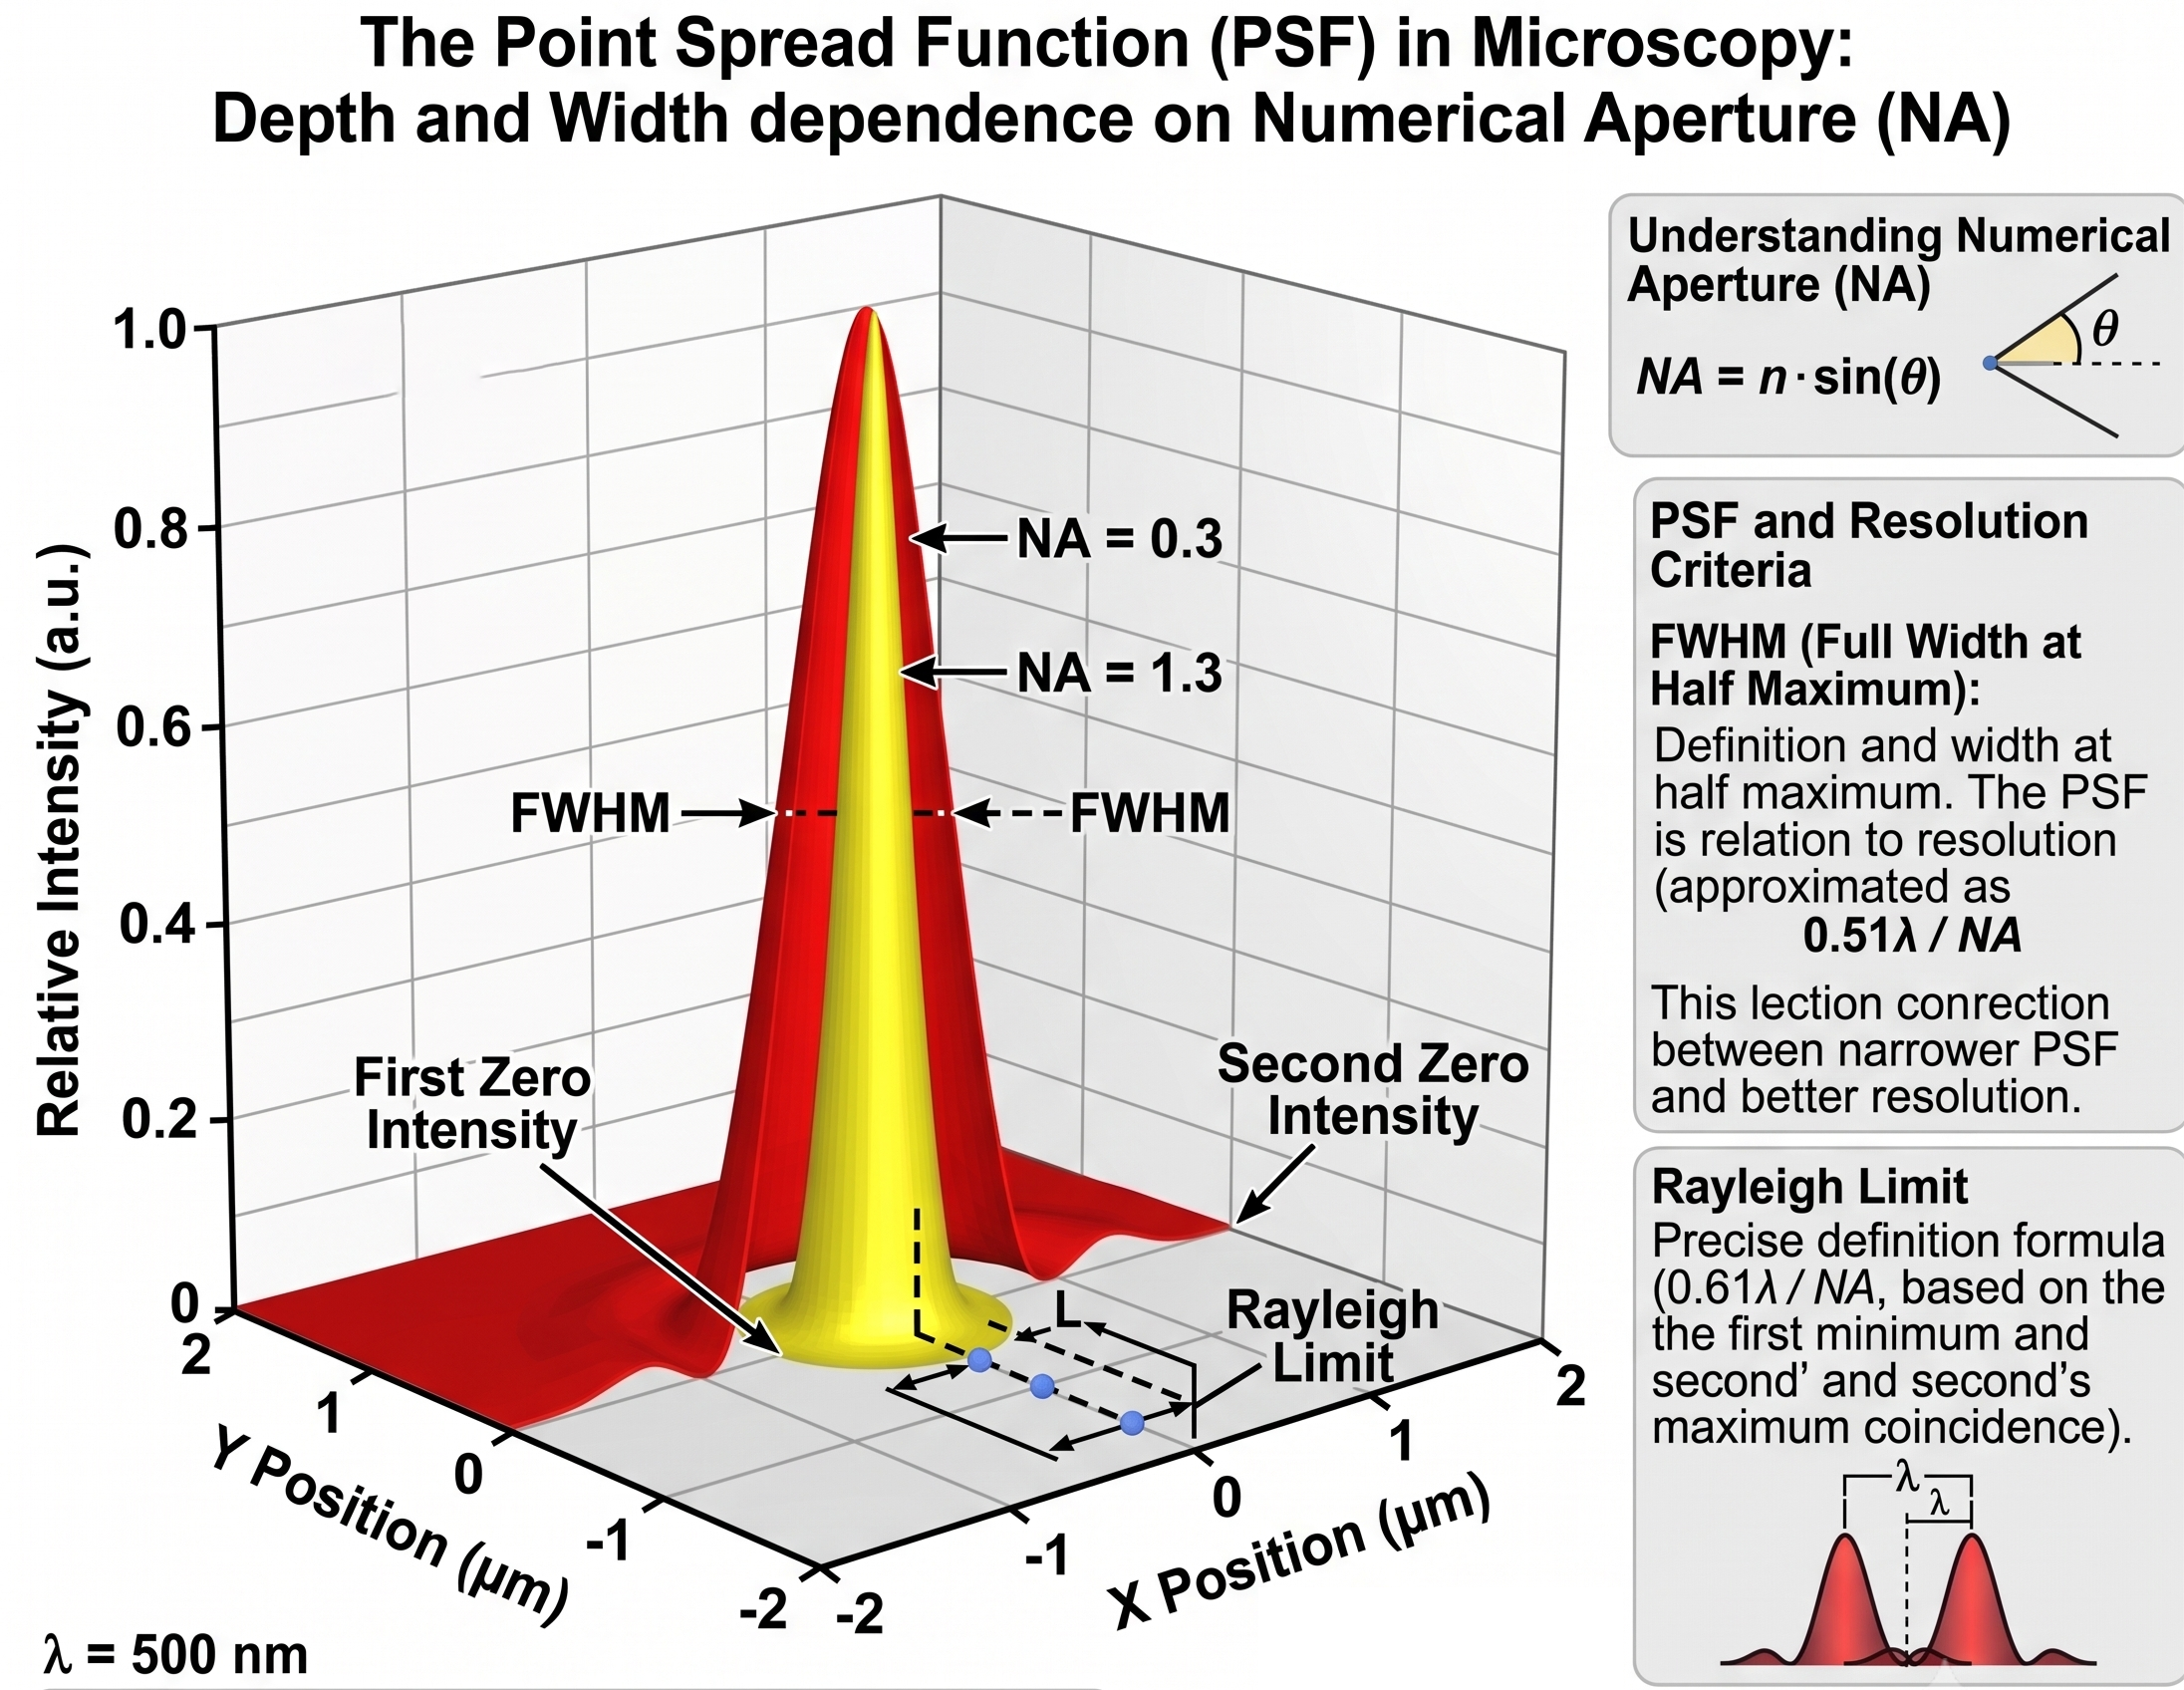
\includegraphics[width=.94\textwidth,height=.42\textheight,keepaspectratio]{Figure/PSF_01.png}
                \caption{PSF、FWHM 与 NA 的关系}
                \label{fig:psf_na_main}
            \end{figure}
        \end{column}
        \hfill
        \begin{column}{.58\textwidth}
            \begin{figure}
                \centering
                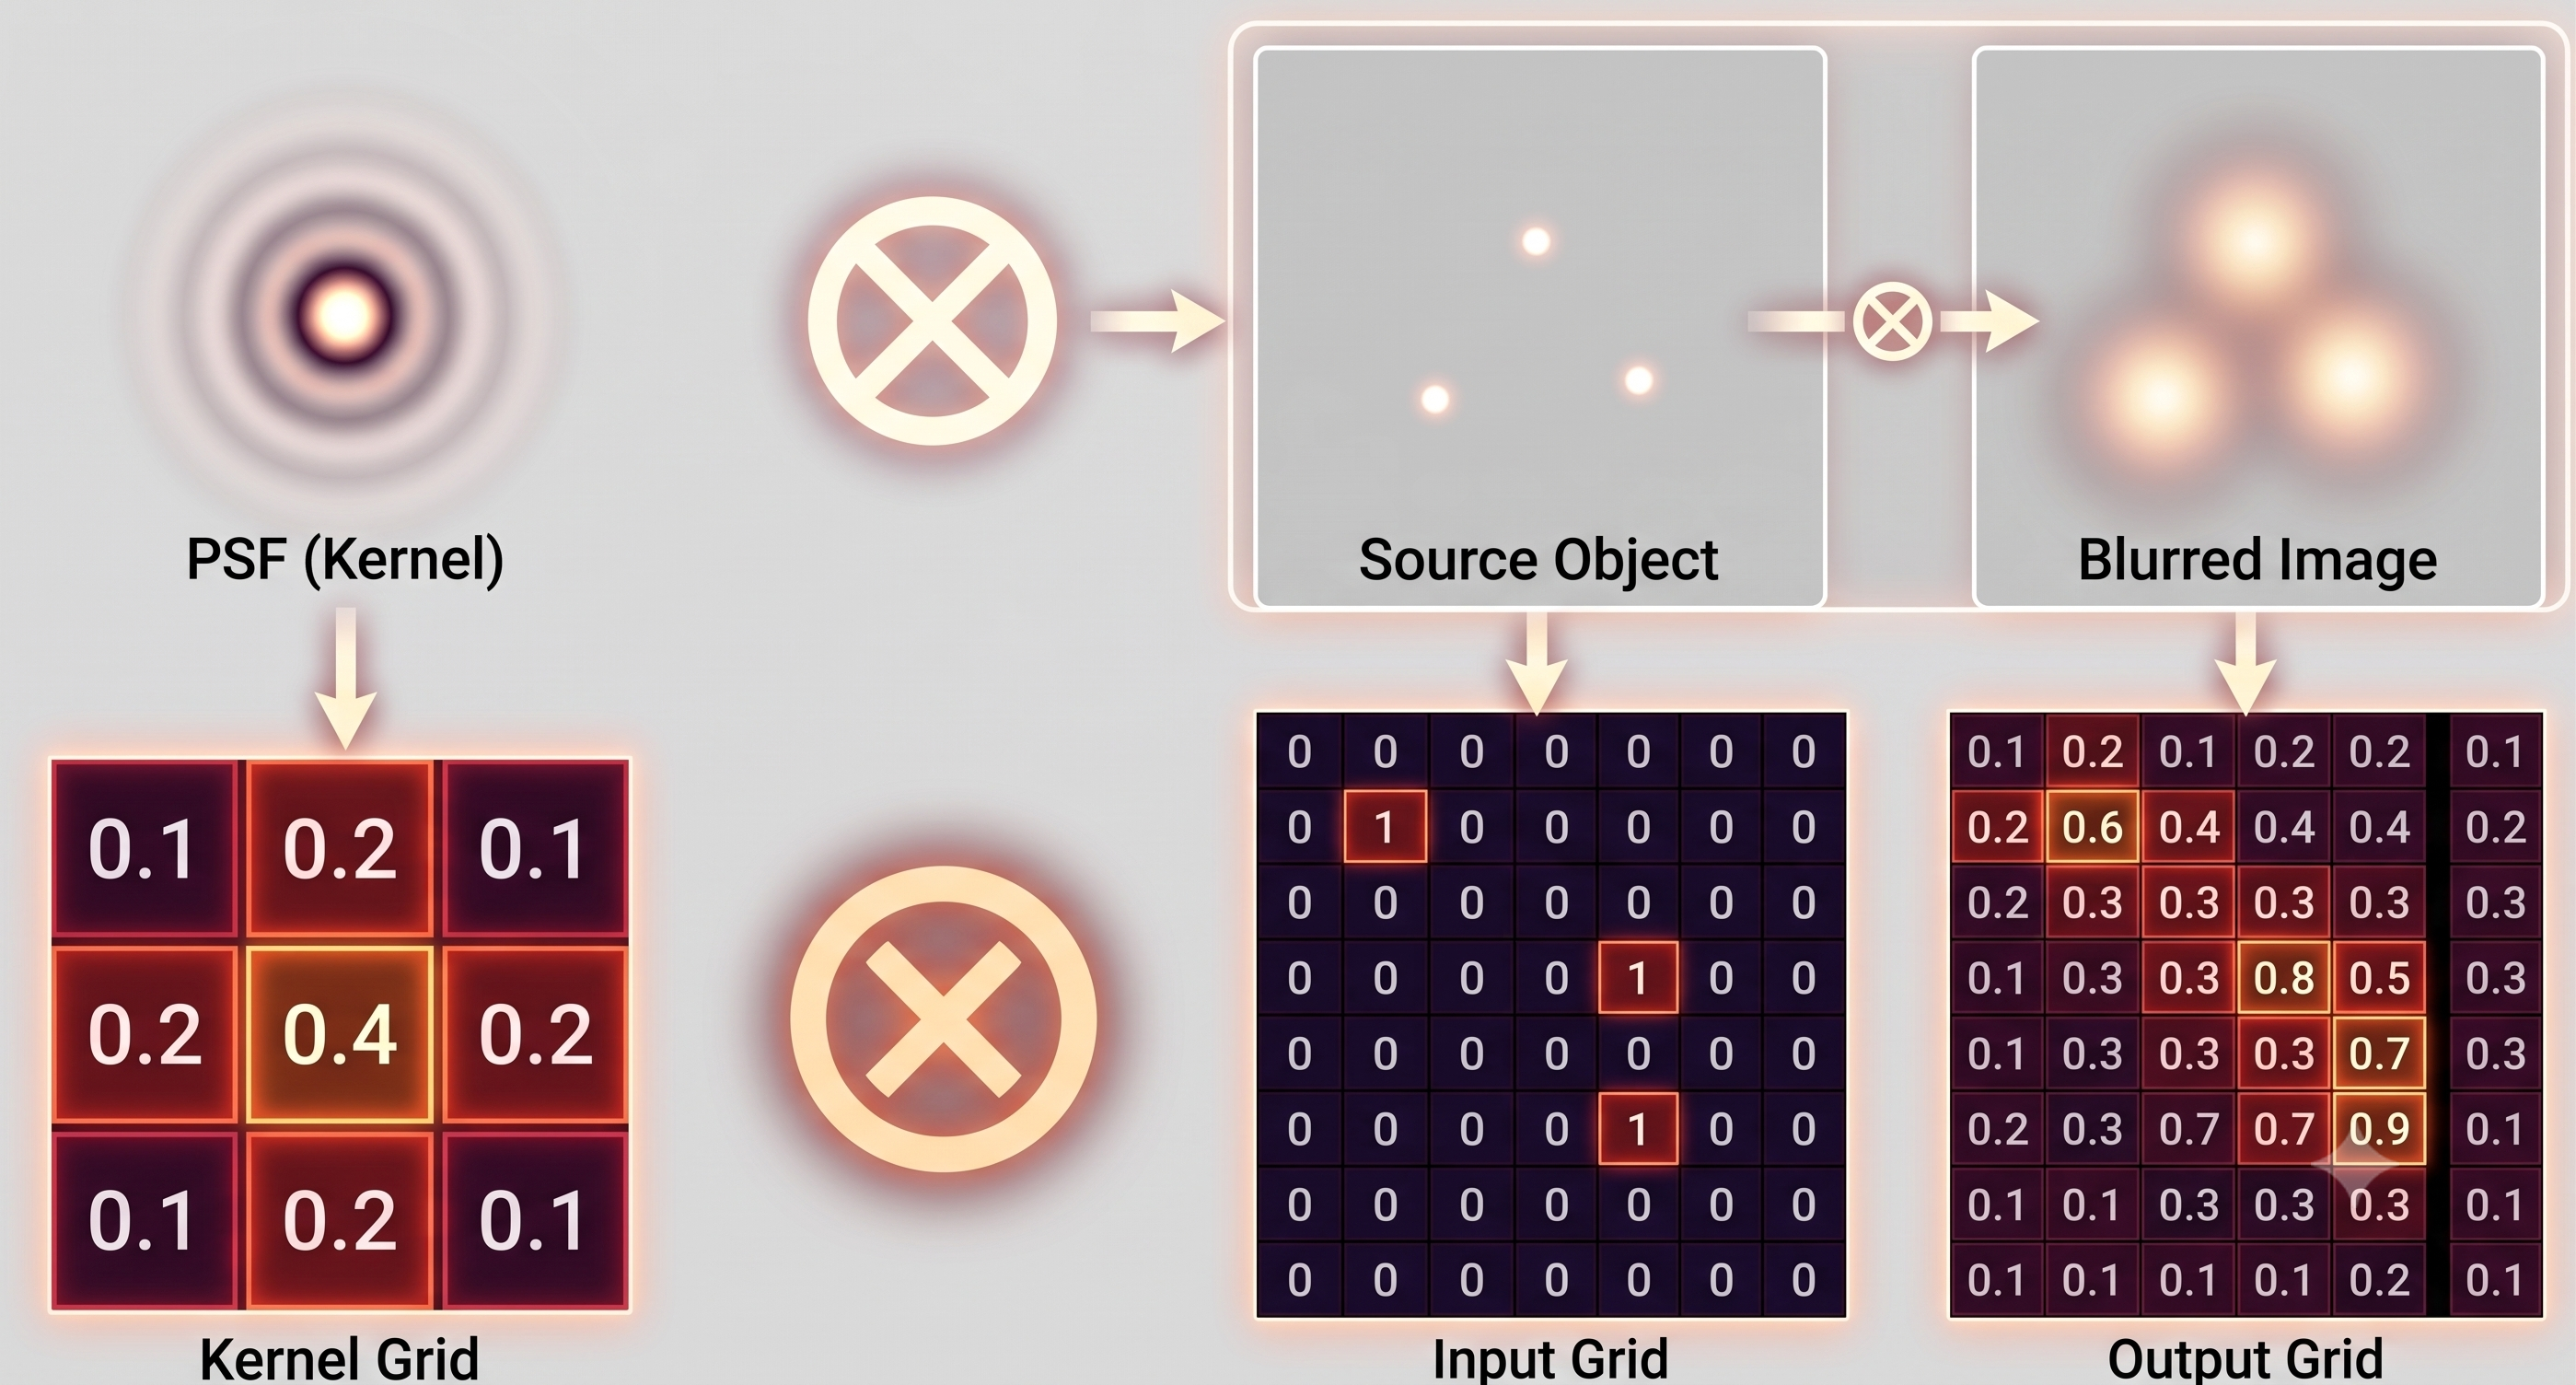
\includegraphics[width=.96\textwidth,height=.30\textheight,keepaspectratio]{Figure/PSF_02.png}
                \caption{物体与 PSF 卷积形成退化图像}
                \label{fig:psf_conv_main}
            \end{figure}

            \vspace{-4pt}
            \begin{equation}
                PSF=\left|\mathcal{F}\{P(\rho,\theta)\}\right|^2,
                \qquad i=o\otimes PSF
                \label{eq:psf_conv_main}
            \end{equation}

            \begin{equation}
                r_{\text{Airy}} = \frac{0.61\lambda}{NA}, \qquad
                OTF=\mathcal{F}\{PSF\}
                \label{eq:airy_otf_main}
            \end{equation}
        \end{column}
    \end{columns}
\end{frame}

\englishtitle{Ray Fan Plot and Its Geometric Meaning}
\begin{frame}{横向像差图：从入瞳采样到像面落点}
\label{1.5}
    \begin{columns}[T]
        \begin{column}{.50\textwidth}
            \begin{figure}
                \centering
                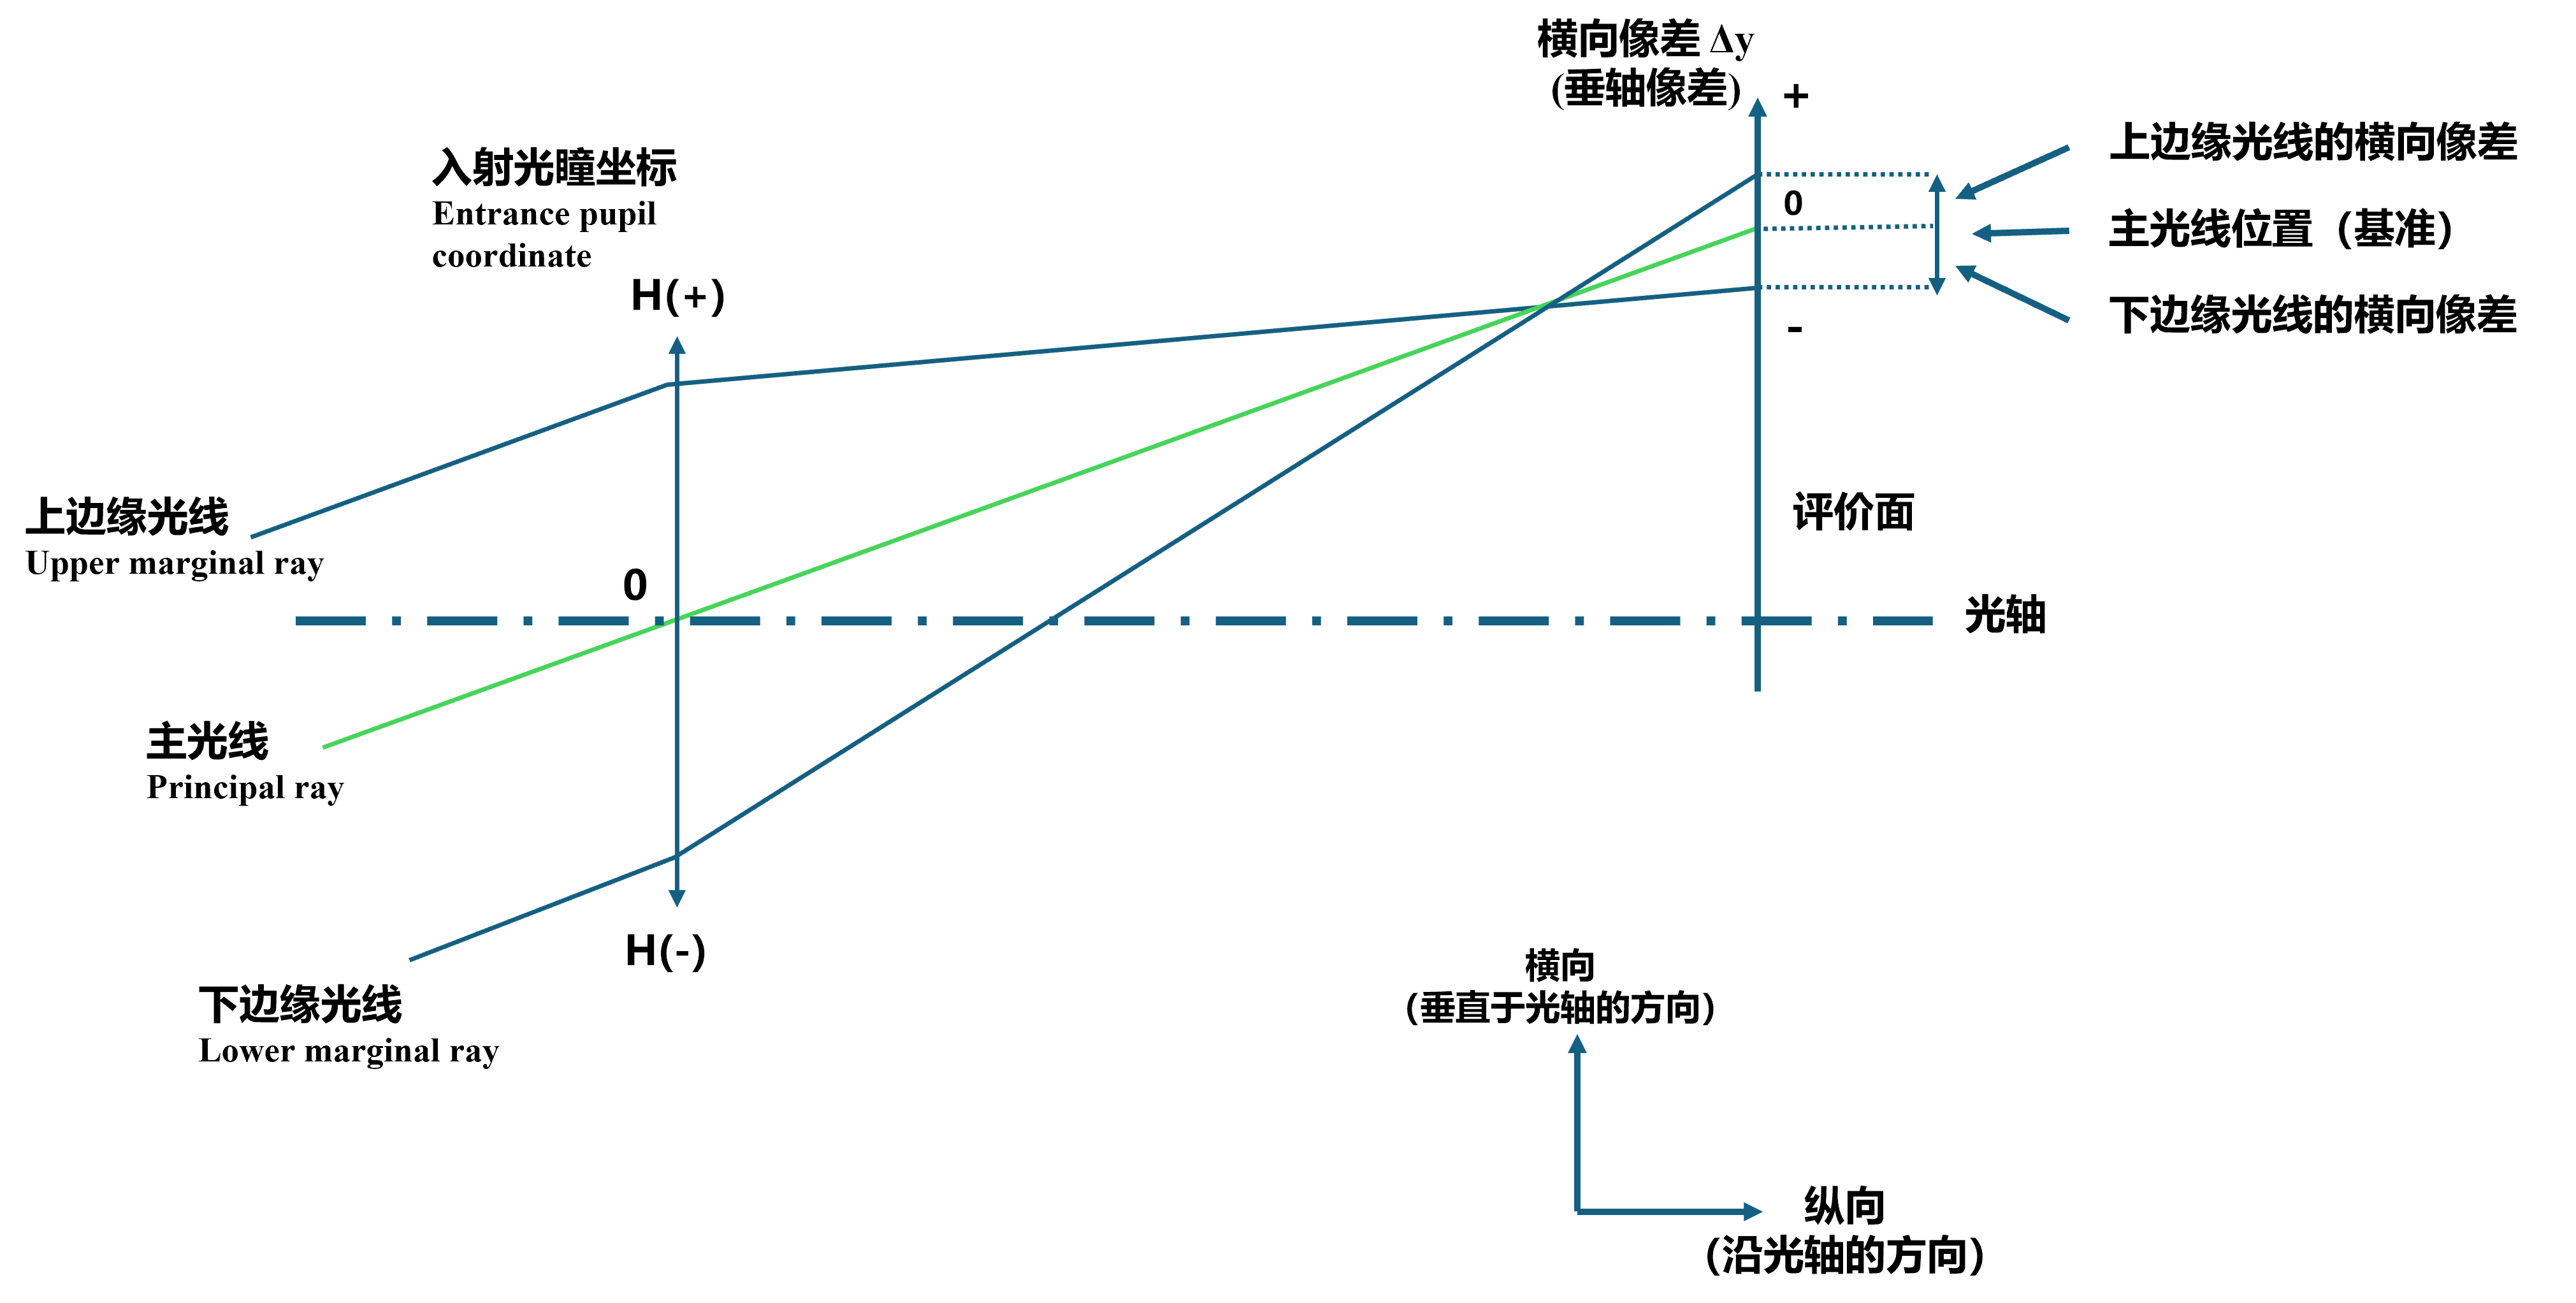
\includegraphics[width=\textwidth,height=.58\textheight,keepaspectratio]{Figure/图片1.png}
                \caption{光线穿过入瞳并落到评估面的几何关系}
                \label{fig:rayfan_ray_geometry_main}
            \end{figure}
        \end{column}
        \hfill
        \begin{column}{.50\textwidth}
            \begin{block}{Ray Fan 的读图方式}
                横轴是归一化入瞳坐标 $h\in[-1,1]$，纵轴是每条光线在评估面上的横向偏移，通常以主光线落点为原点。
            \end{block}

            \begin{itemize}
                \item \textbf{曲线斜率}：主要对应离焦、场曲、像散等线性项。
                \item \textbf{曲线弯曲}：对应球差、彗差等高阶项。
                \item \textbf{视场变化}：区分轴上像差和轴外像差。
                \item \textbf{波长变化}：区分单色像差和色差。
            \end{itemize}

            \alert{Ray Fan 是几何诊断图；PSF 是最终点像能量分布。两者相关，但不能混用图片和结论。}
        \end{column}
    \end{columns}
\end{frame}

\englishtitle{Ideal Imaging and Defocus}
\begin{frame}{理想成像与离焦}
\label{1.6}
    \begin{figure}
        \centering
        \begin{minipage}[t]{.32\textwidth}
            \centering
            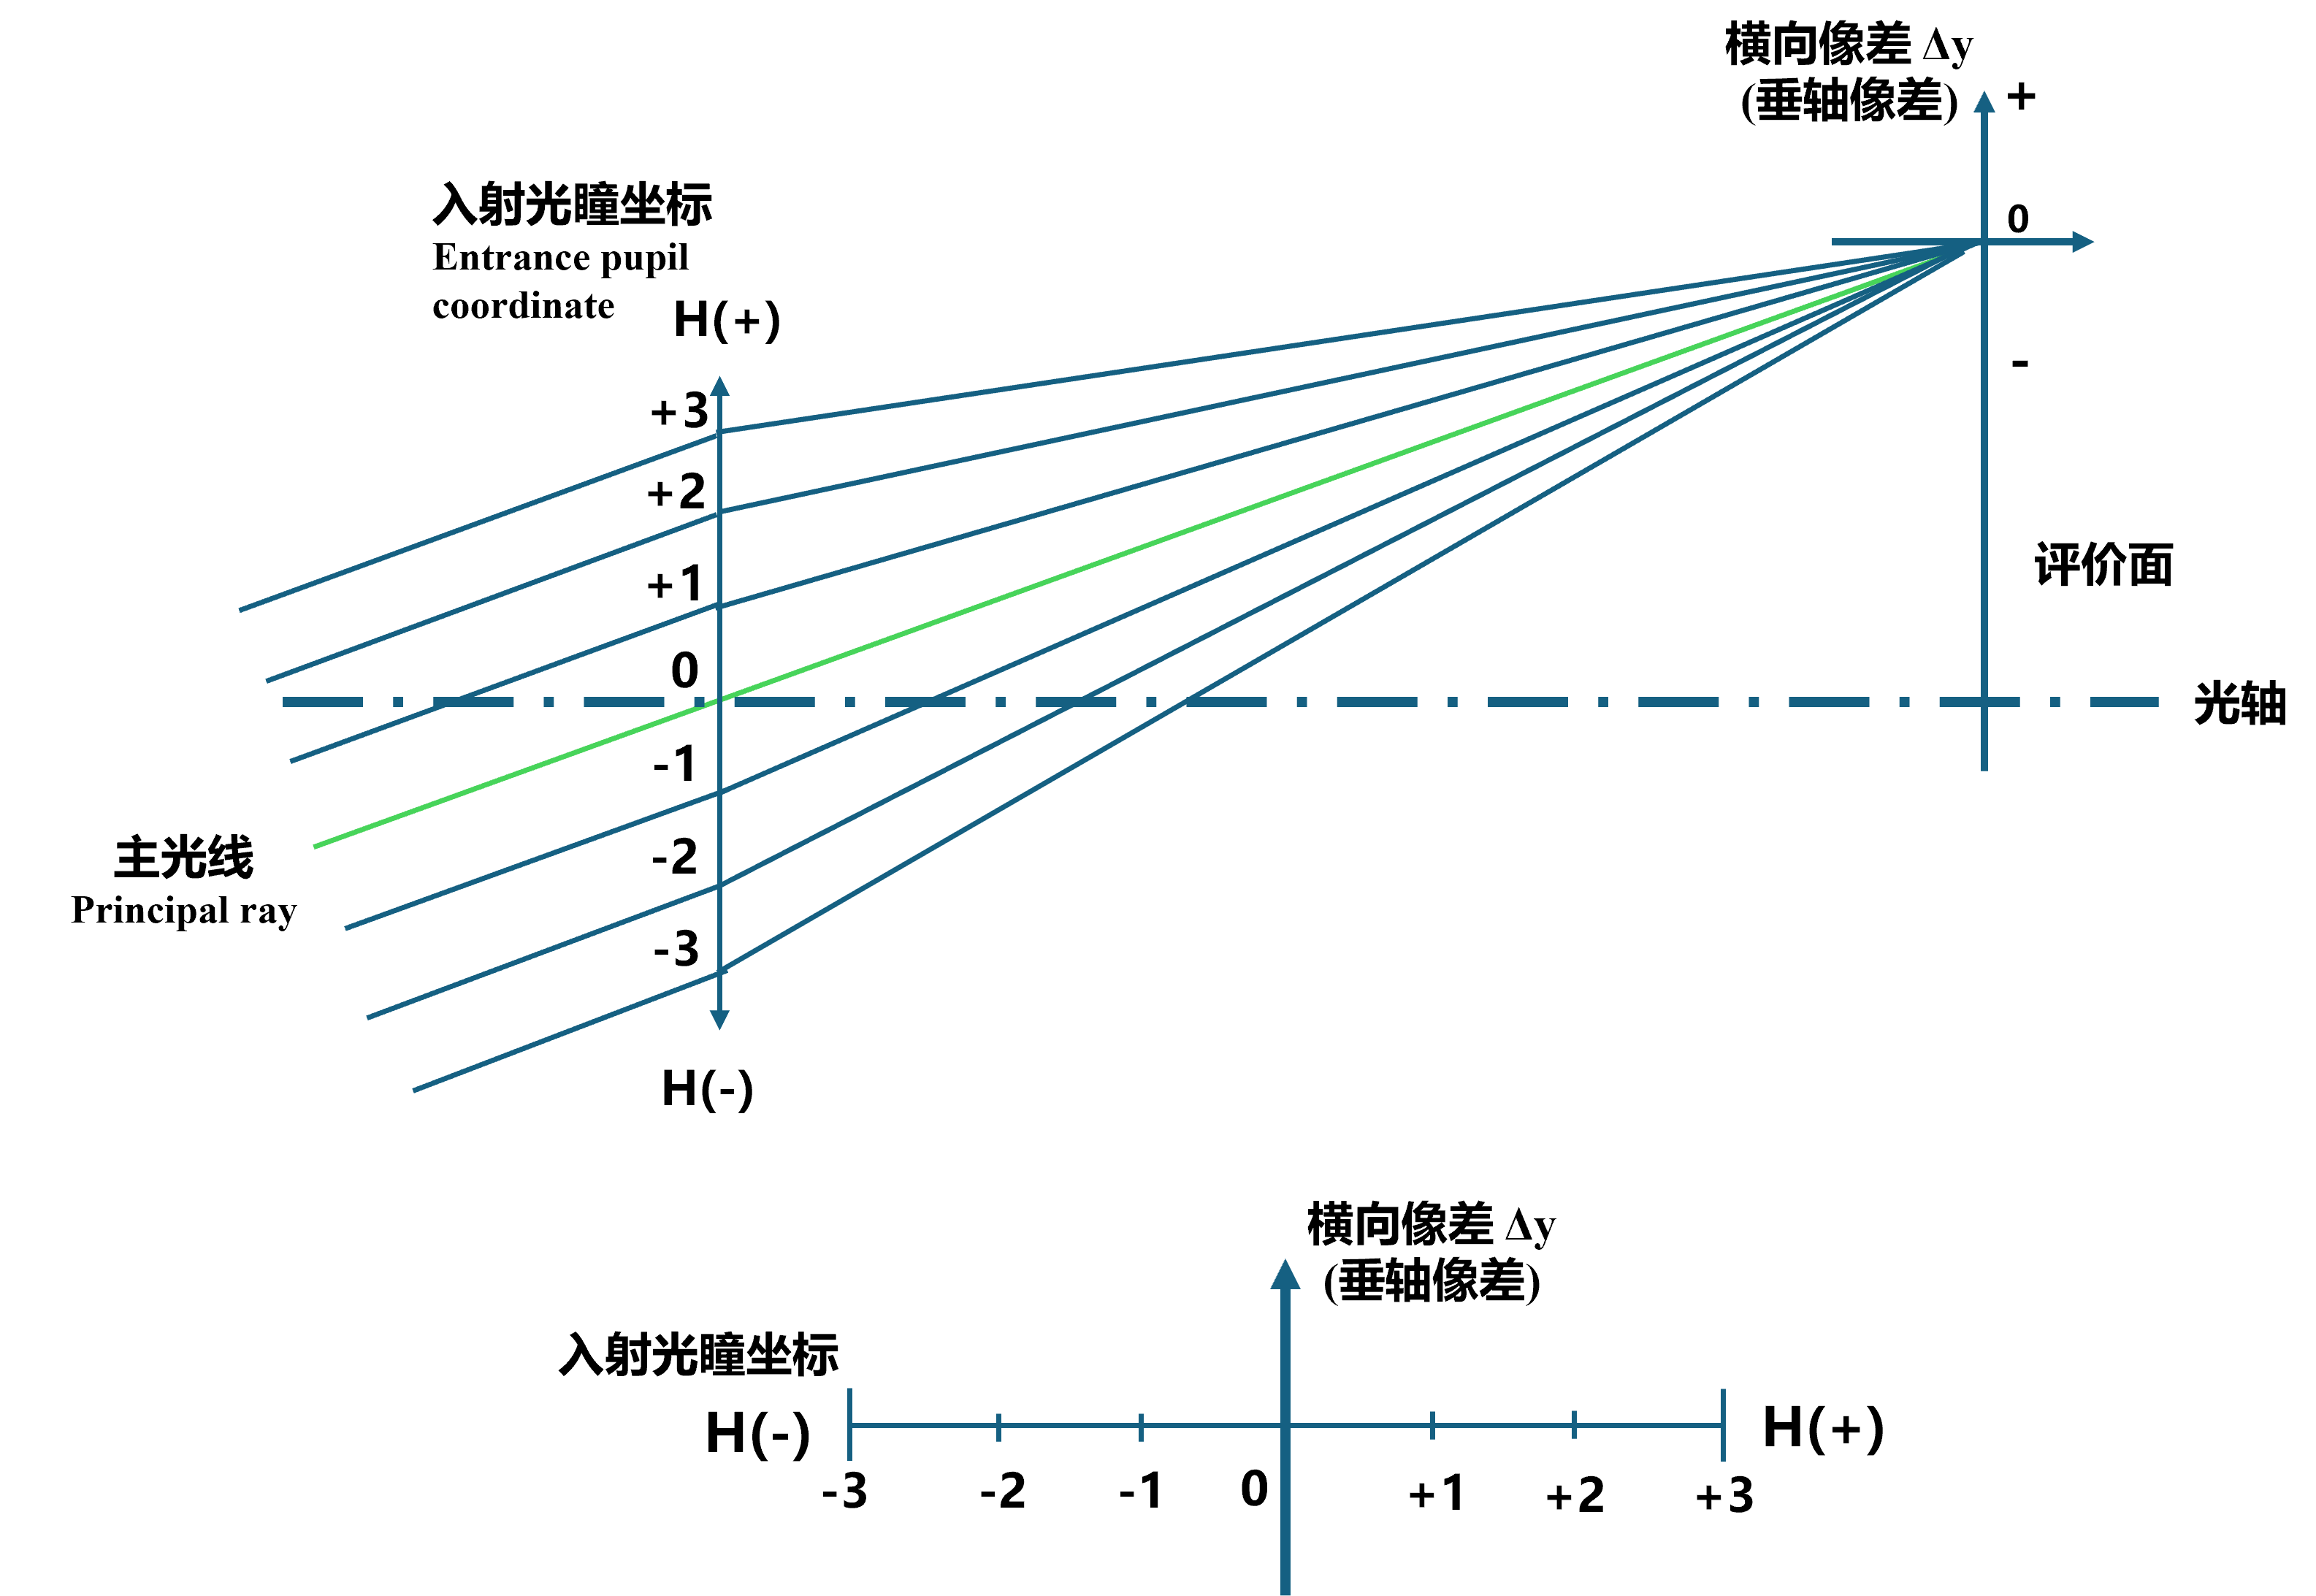
\includegraphics[width=\linewidth,height=.40\textheight,keepaspectratio]{Figure/图片3.png}
            \scriptsize 理想评估面：所有光线会聚于同一点
        \end{minipage}
        \hfill
        \begin{minipage}[t]{.32\textwidth}
            \centering
            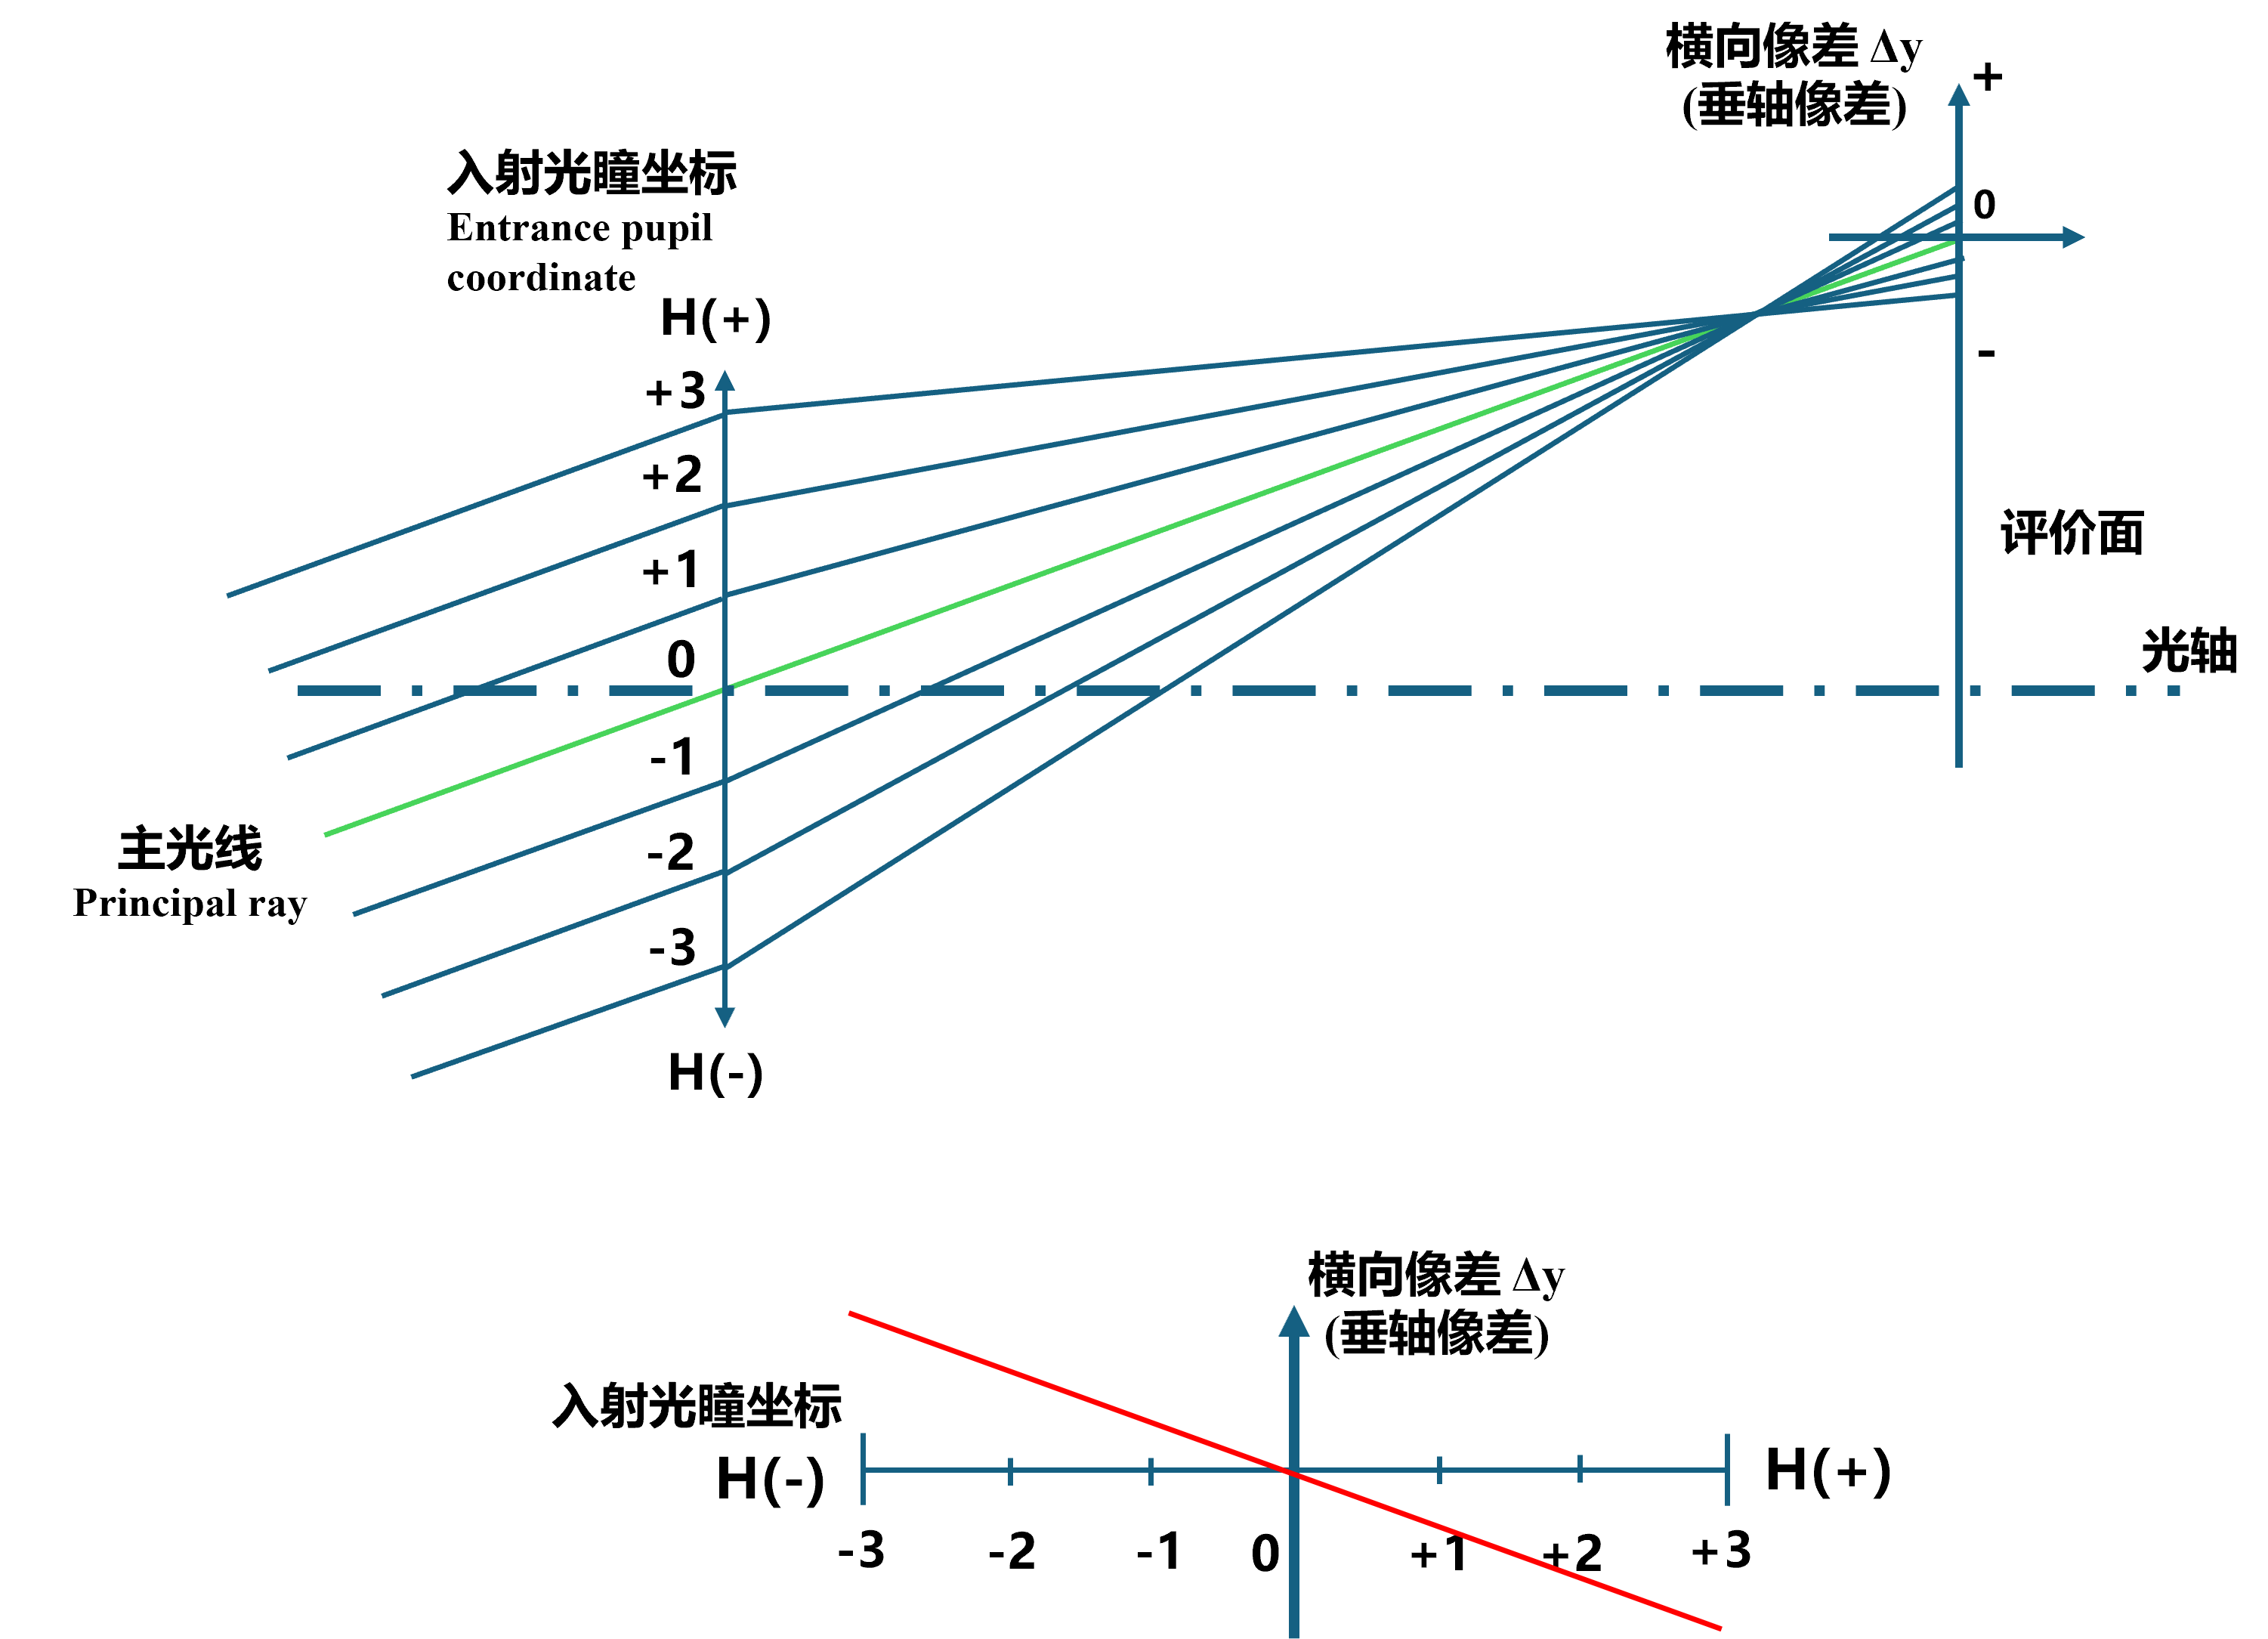
\includegraphics[width=\linewidth,height=.40\textheight,keepaspectratio]{Figure/图片4.png}
            \scriptsize 评估面远离最佳焦面：Ray Fan 呈一侧倾斜直线
        \end{minipage}
        \hfill
        \begin{minipage}[t]{.32\textwidth}
            \centering
            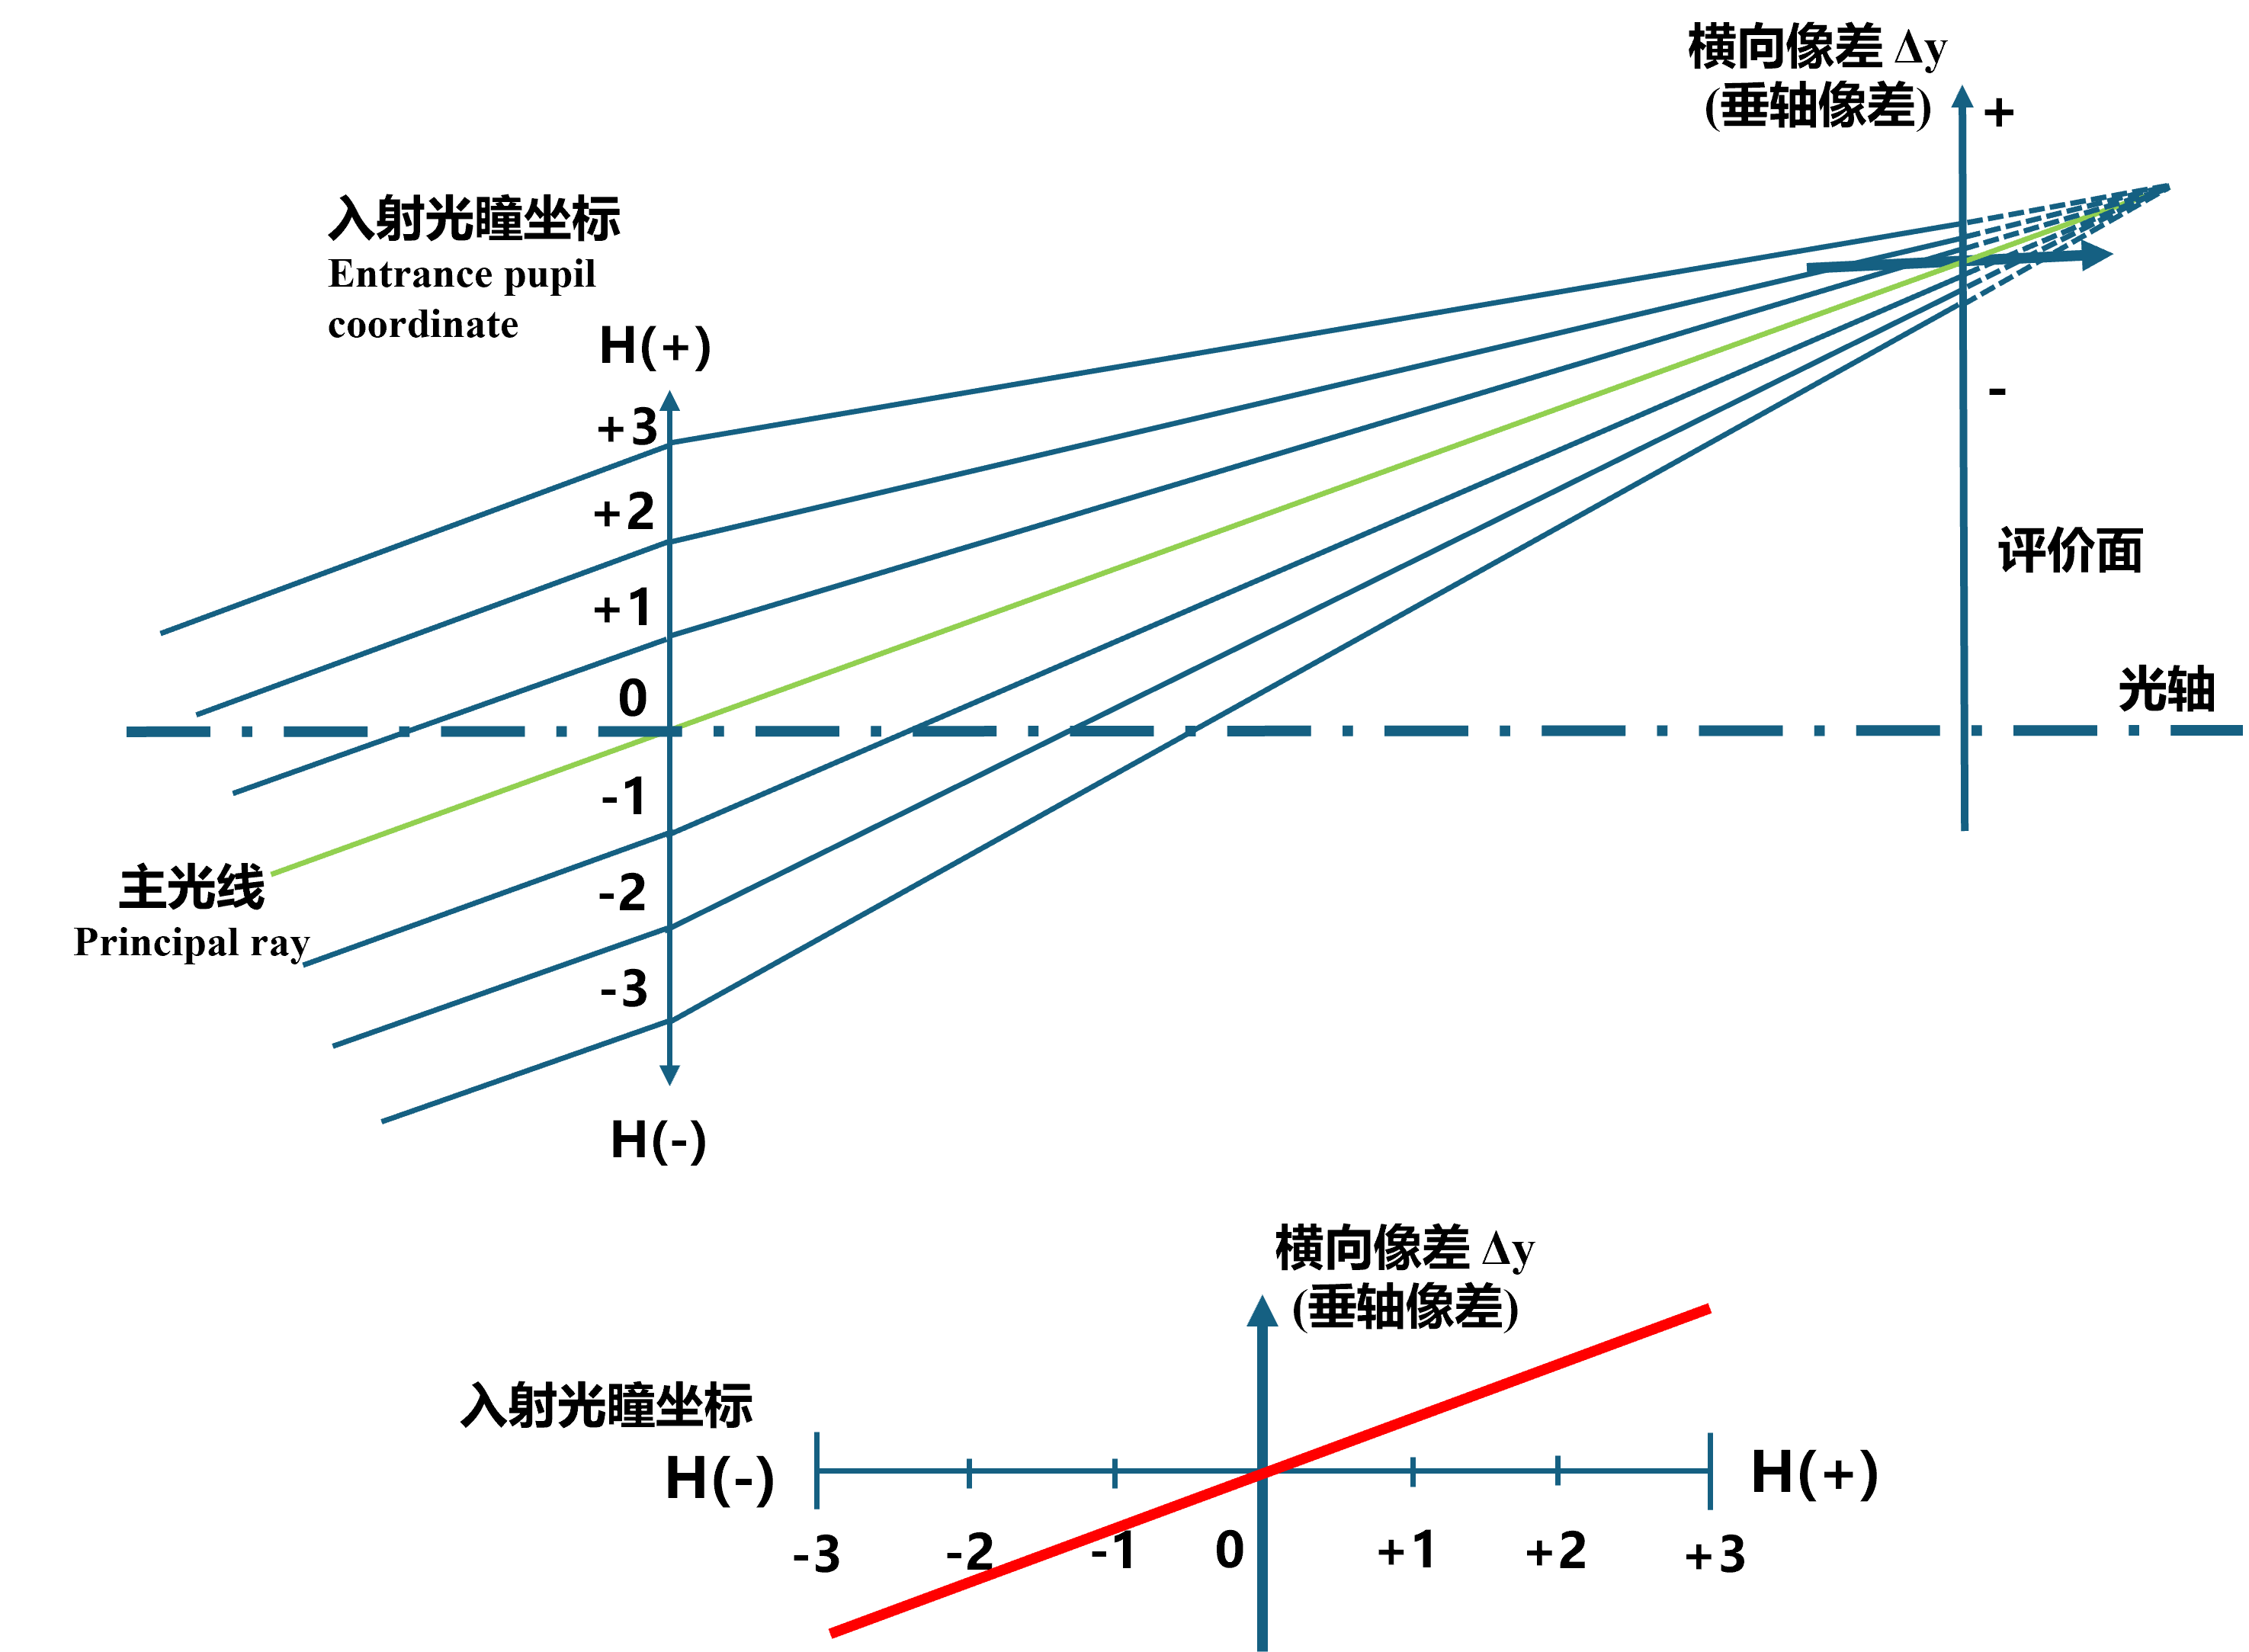
\includegraphics[width=\linewidth,height=.40\textheight,keepaspectratio]{Figure/图片6.png}
            \scriptsize 评估面靠近镜头：斜率方向相反
        \end{minipage}
        \caption{理想成像与正负离焦的统一示意}
        \label{fig:ideal_defocus_merged}
    \end{figure}

    \vspace{-4pt}
    \begin{columns}[T]
        \begin{column}{.50\textwidth}
            \begin{itemize}
                \item 无像差：横向像差为零，Ray Fan 落在横轴上。
                \item 离焦：Ray Fan 是通过原点的直线。
            \end{itemize}
        \end{column}
        \begin{column}{.50\textwidth}
            \begin{itemize}
                \item 改变像面位置只能消除线性离焦项。
                \item 弯曲项仍存在时，需要改变光学结构或面形。
            \end{itemize}
        \end{column}
    \end{columns}
\end{frame}

\subsection{Seidel 像差与 Zernike 展开}
\label{sec:1.3}

\englishtitle{Third-Order Aberration as Residual After Paraxial Imaging}
\begin{frame}{三阶像差：理想成像之后的最低阶残差}
\label{1.7}
    \small
    \textbf{在一阶成像已经确定之后，Ray Fan 的最低阶残差可写成：}
    \begin{equation}
        \Delta y(h,\omega)
        \approx A h
        + B h^3
        + C h^2\tan\omega
        + D h\tan^2\omega
        + E\tan^3\omega
        \label{eq:rayfan_third_order}
    \end{equation}

    \vspace{-2pt}
    \begin{table}
        \centering
        \scriptsize
        \renewcommand{\arraystretch}{1.25}
        \begin{tabular}{p{2.1cm}|p{2.2cm}|p{2.5cm}|p{4.5cm}}
            \toprule
            \textbf{项} & \textbf{孔径依赖} & \textbf{视场依赖} & \textbf{Ray Fan 诊断特征} \\
            \midrule
            离焦 & $h$ & 与视场弱相关 & 通过原点的直线，移动像面可改变斜率 \\
            球差 & $h^3$ & 轴上存在 & 奇函数三次曲线，边缘孔径贡献最大 \\
            彗差 & $h^2$ & $\tan\omega$ & 偶函数二次曲线，离轴视场快速变坏 \\
            像散/场曲 & $h$ & $\tan^2\omega$ & 原点附近斜率随视场或子午/弧矢方向改变 \\
            畸变 & $h^0$ & $\tan^3\omega$ & 主光线像高偏移，Ray Fan 不直接显示弥散形状 \\
            \bottomrule
        \end{tabular}
        \caption{三阶项与横向像差图的对应关系}
        \label{tab:third_order_rayfan_main}
    \end{table}

    \alert{合并后的理解：}一阶量负责把像“放到正确位置”；三阶项描述“放到那里之后还剩下什么形状的误差”。
\end{frame}

\englishtitle{Zernike Polynomial Expansion}
\begin{frame}{Zernike 多项式：波前像差的正交坐标系}
\label{1.8}
    \begin{columns}[T]
        \begin{column}{.52\textwidth}
            对圆形光瞳，波像差通常展开为：
            \begin{equation}
                W(\rho,\theta)=\sum_j C_j Z_j(\rho,\theta),
                \qquad 0\le \rho \le 1
                \label{eq:zernike_main}
            \end{equation}

            \begin{equation}
                Z_n^m(\rho,\theta)
                =R_n^m(\rho)\cos(m\theta)
                \ \text{或}\
                R_n^m(\rho)\sin(m\theta)
                \label{eq:zernike_nm_main}
            \end{equation}

            \begin{equation}
                \int_0^1\!\!\int_0^{2\pi}
                Z_i Z_j\,\rho\,d\theta\,d\rho
                = N_i\delta_{ij}
                \label{eq:zernike_orthogonal_main}
            \end{equation}
        \end{column}
        \hfill
        \begin{column}{.48\textwidth}
            \begin{itemize}
                \item Zernike直接面向\alert{波前 $W$}，比单纯看 Ray Fan 更接近像质根源。
                \item 正交性让每个系数 $C_j$ 具有相对独立的含义，便于量化比较。
                \item Zemax 的 Wavefront Map、Zernike Standard Coefficients 和 RMS Wavefront 都建立在同一套波前语言上。
                \item 干涉仪测量、自由曲面补偿和自适应光学校正也常用 Zernike 系数沟通。
            \end{itemize}

            \begin{alertblock}{从波前到光线}
                Ray Fan 可近似理解为波前斜率的表现：
                \[
                    \Delta \mathbf{r}_{\perp}\propto \nabla_{\rho,\theta} W
                \]
            \end{alertblock}
        \end{column}
    \end{columns}
\end{frame}

\englishtitle{Zernike Modes and Physical Aberrations}
\begin{frame}{常用 Zernike 模式与像差含义}
\label{1.9}
    \scriptsize
    \begin{table}
        \centering
        \renewcommand{\arraystretch}{1.42}
        \begin{tabular}{p{2.3cm}|p{3.2cm}|p{3.0cm}|p{3.4cm}}
            \toprule
            \textbf{Zernike 模式} & \textbf{典型形式} & \textbf{物理含义} & \textbf{诊断用途} \\
            \midrule
            Piston & $1$ & 整体相位常数 & 不影响成像，通常去除 \\
            Tilt X/Y & $\rho\cos\theta,\ \rho\sin\theta$ & 像点平移或装调倾斜 & 通常作为对准误差处理 \\
            Defocus & $2\rho^2-1$ & 像面前后移动 & 与 Ray Fan 直线斜率对应 \\
            Astigmatism & $\rho^2\cos2\theta,\ \rho^2\sin2\theta$ & 两个正交方向焦点不同 & 区分子午与弧矢焦面 \\
            Coma & $(3\rho^3-2\rho)\cos\theta$ 等 & 轴外不对称波前 & 对应 Ray Fan 二次弯曲 \\
            Primary spherical & $6\rho^4-6\rho^2+1$ & 边缘与近轴光线焦点不同 & 对应轴上三次型 Ray Fan \\
            Higher order terms & $n\ge5$ & 高阶球差、二级彗差等 & 大 NA、自由曲面或复杂系统中需关注 \\
            \bottomrule
        \end{tabular}
        \caption{Zernike 系数不是装饰性输出，而是可用于优化、测量和误差分解的波前坐标}
        \label{tab:zernike_modes_main}
    \end{table}

    \vspace{-2pt}
    \begin{block}{使用建议}
        先移除 piston、tilt 和必要的 defocus，再讨论剩余 Zernike 系数；否则装调误差和像面位置会掩盖真正的设计像差。
    \end{block}
\end{frame}

\subsection{单色像差诊断：先分清曲线形状}
\label{sec:1.4}

\englishtitle{Monochromatic Aberrations in Ray Fan}
\begin{frame}{球差、彗差与离焦：先看曲线阶次}
\label{1.10}
    \begin{figure}
        \centering
        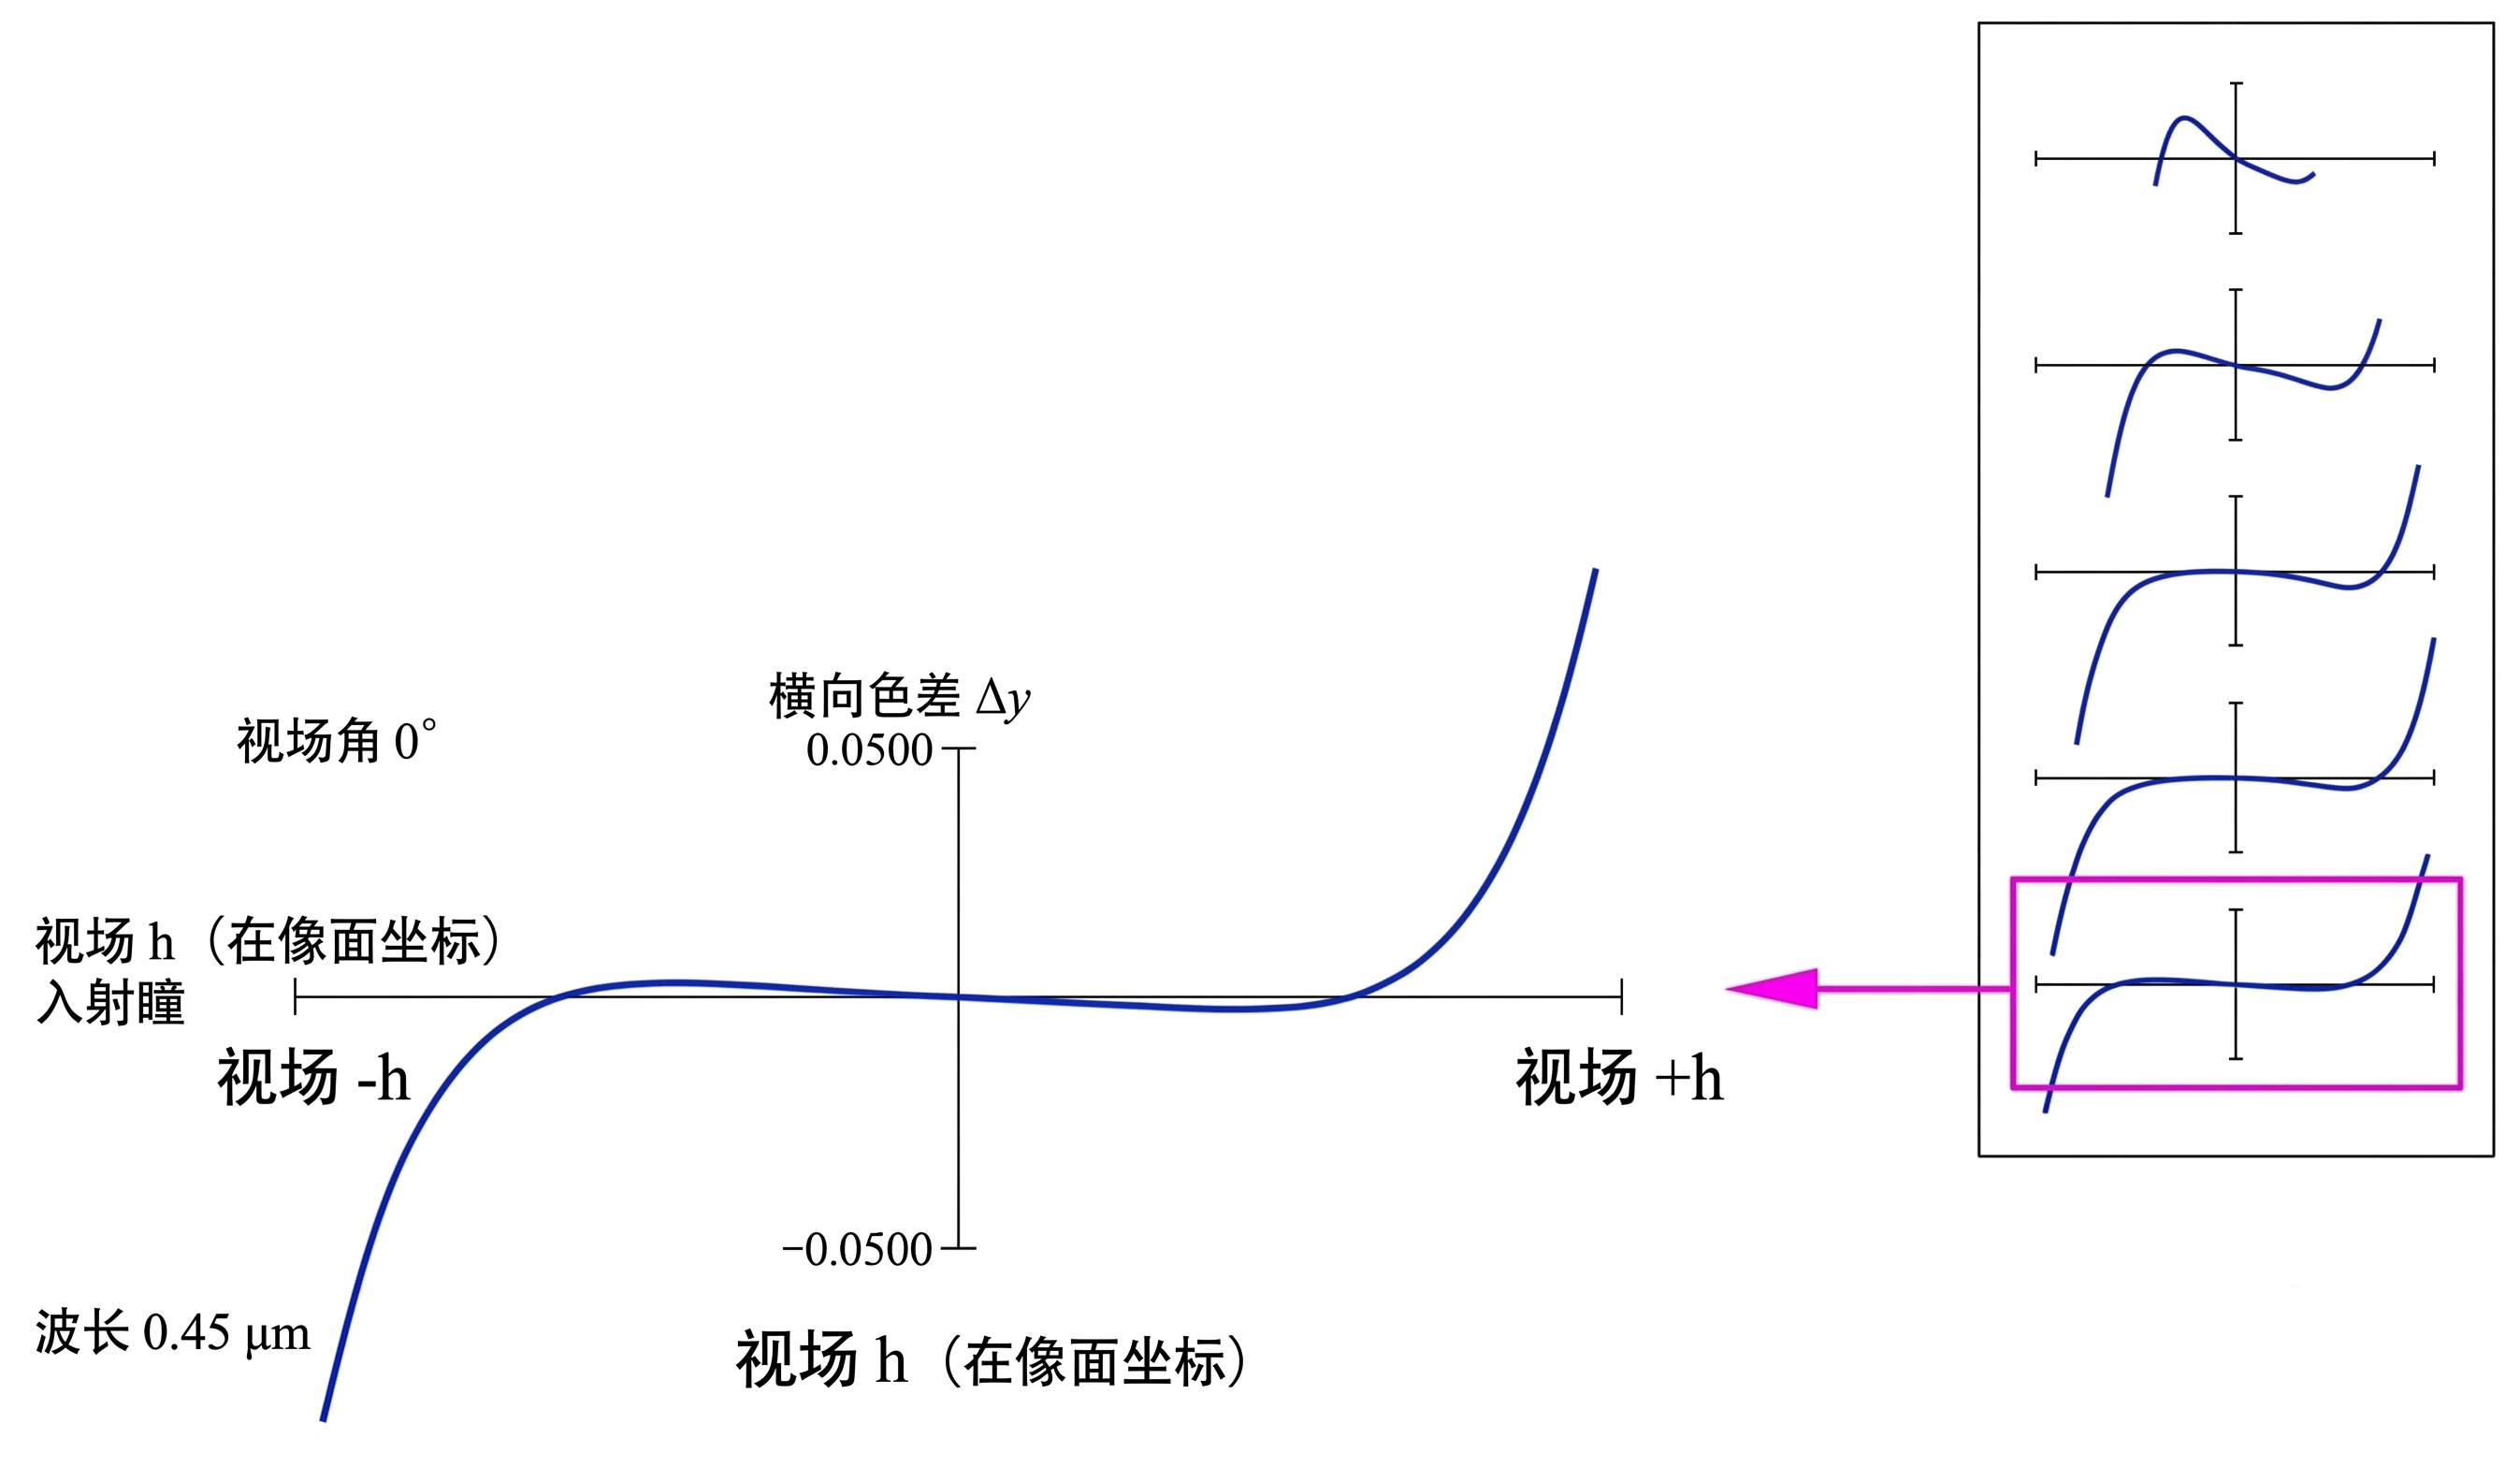
\includegraphics[width=.48\textwidth,height=.28\textheight,keepaspectratio]{Figure/图片23.png}\hfill
        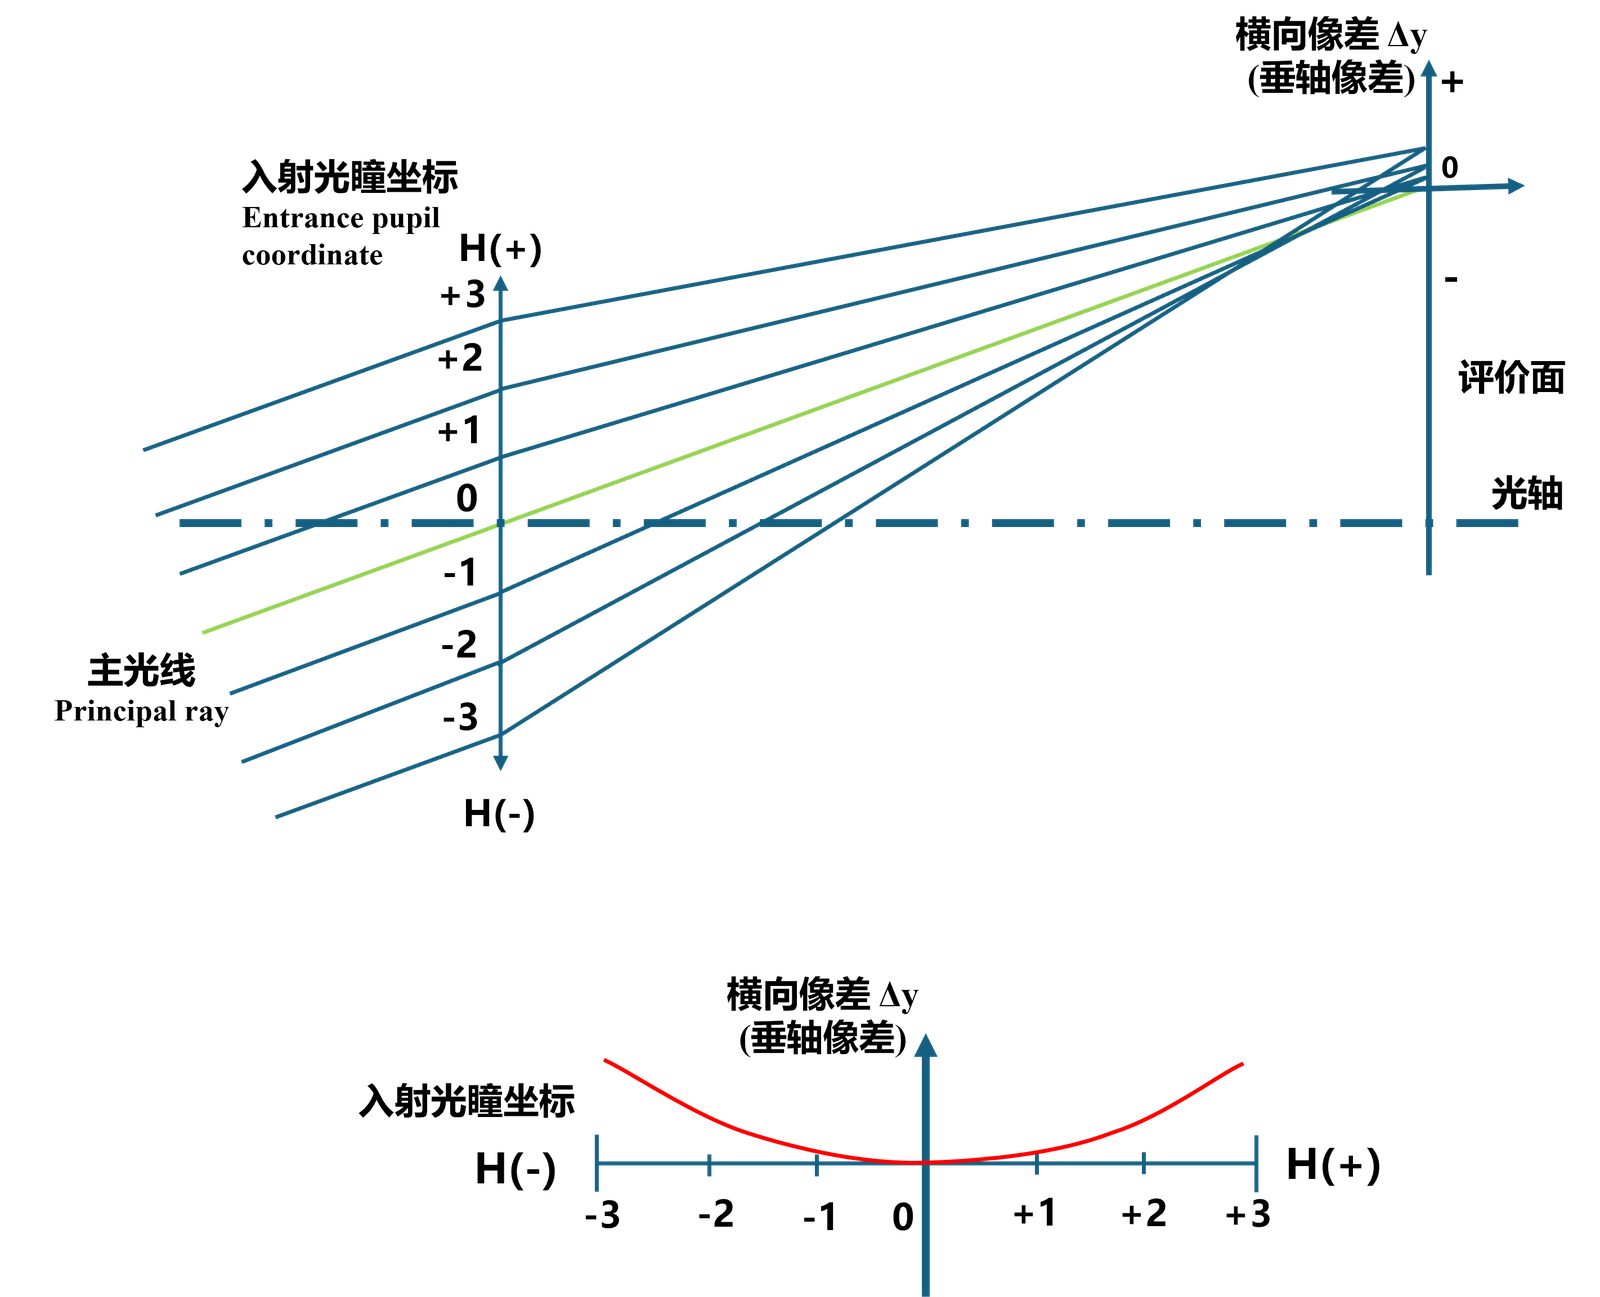
\includegraphics[width=.23\textwidth,height=.20\textheight,keepaspectratio]{Figure/图片8.png}\hfill
        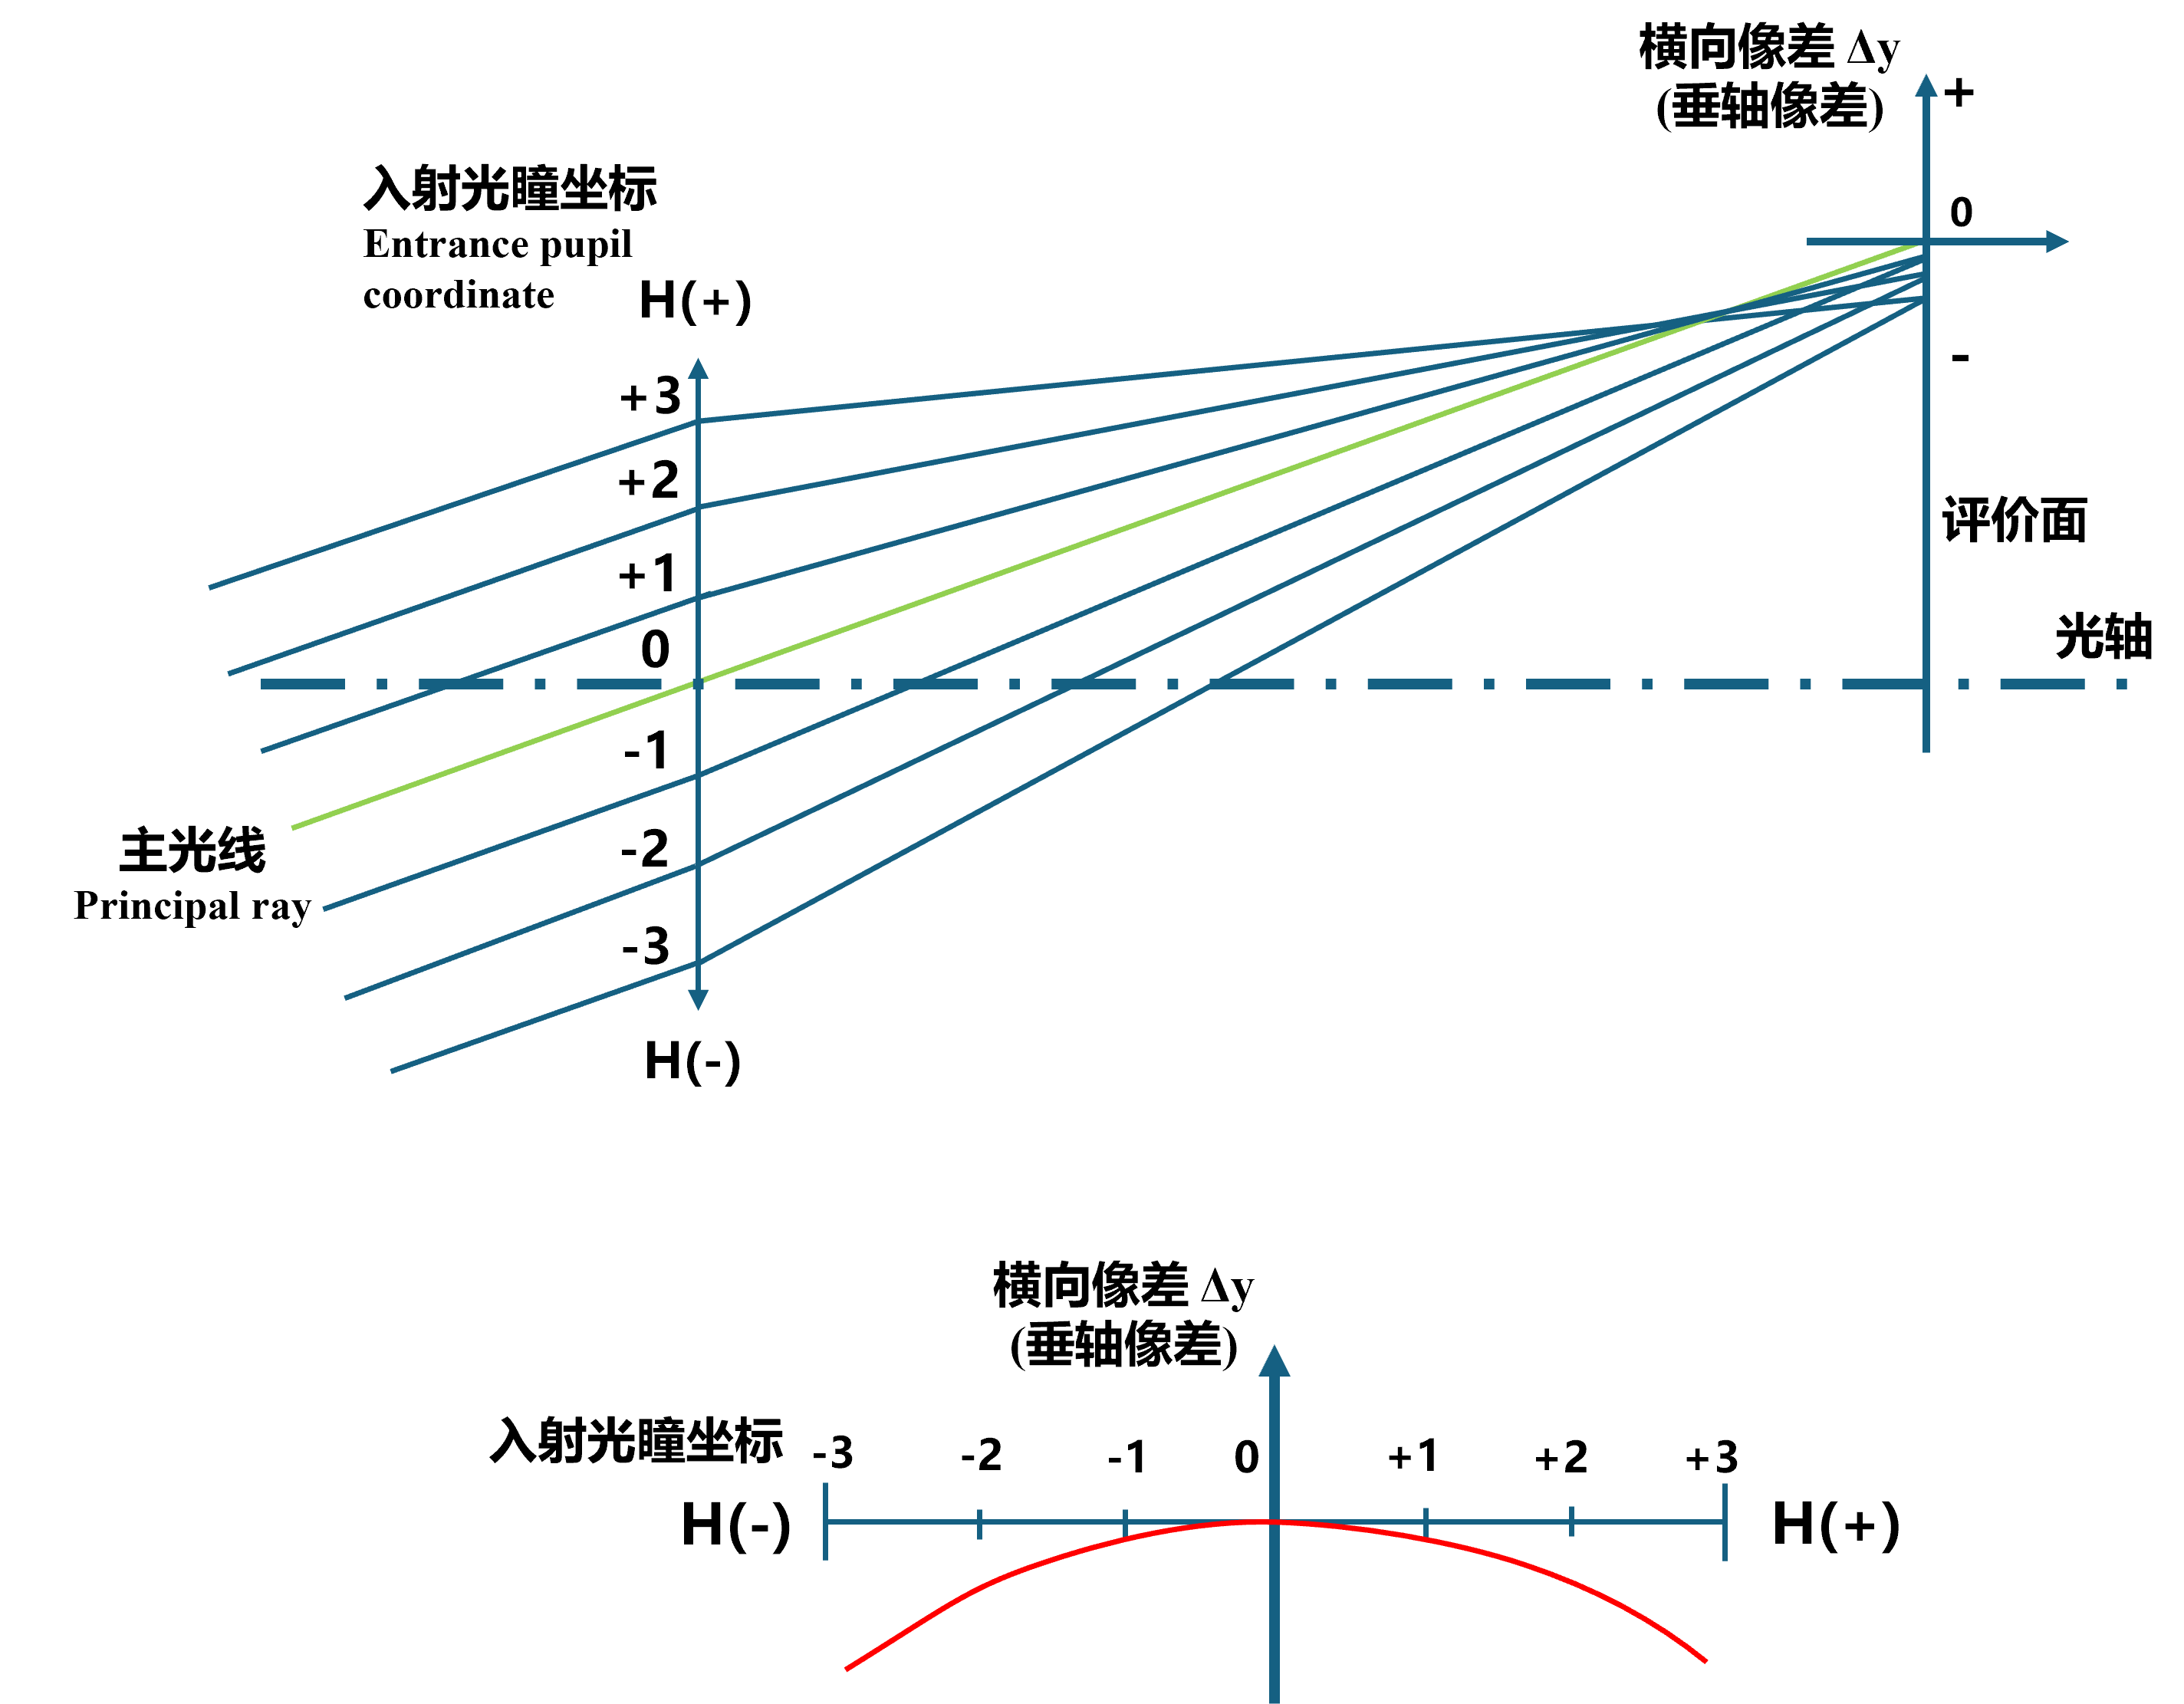
\includegraphics[width=.23\textwidth,height=.20\textheight,keepaspectratio]{Figure/图片11.png}
        \caption{左：球差的三次型 Ray Fan；右：彗差的二次型 Ray Fan，开口方向区分内向/外向}
        \label{fig:spherical_coma_rayfan_main}
    \end{figure}

    \vspace{-4pt}
    \begin{table}
        \centering
        \scriptsize
        \renewcommand{\arraystretch}{1.3}
        \begin{tabular}{p{1.8cm}|p{3.2cm}|p{4.8cm}}
            \toprule
            \textbf{类型} & \textbf{Ray Fan 特征} & \textbf{设计动作} \\
            \midrule
            离焦 & 通过原点的直线 & 先移动像面；若只剩斜率，优先修焦面位置 \\
            球差 & 轴上三次曲线，边缘孔径贡献最大 & 分摊光焦度、改变弯曲因子、引入非球面 \\
            彗差 & 离轴二次曲线，随视场快速增加 & 调整光阑位置、增强结构对称性、降低离轴入射角 \\
            \bottomrule
        \end{tabular}
    \end{table}

    \alert{这一页把原先分散的离焦、球差、彗差合并为一个判据：先看阶次，再决定是移像面还是改结构。}
\end{frame}

\englishtitle{Field Curvature and Astigmatism}
\begin{frame}{场曲与像散：同是斜率问题，但物理来源不同}
\label{1.11}
    \begin{columns}[T]
        \begin{column}{.53\textwidth}
            \begin{figure}
                \centering
                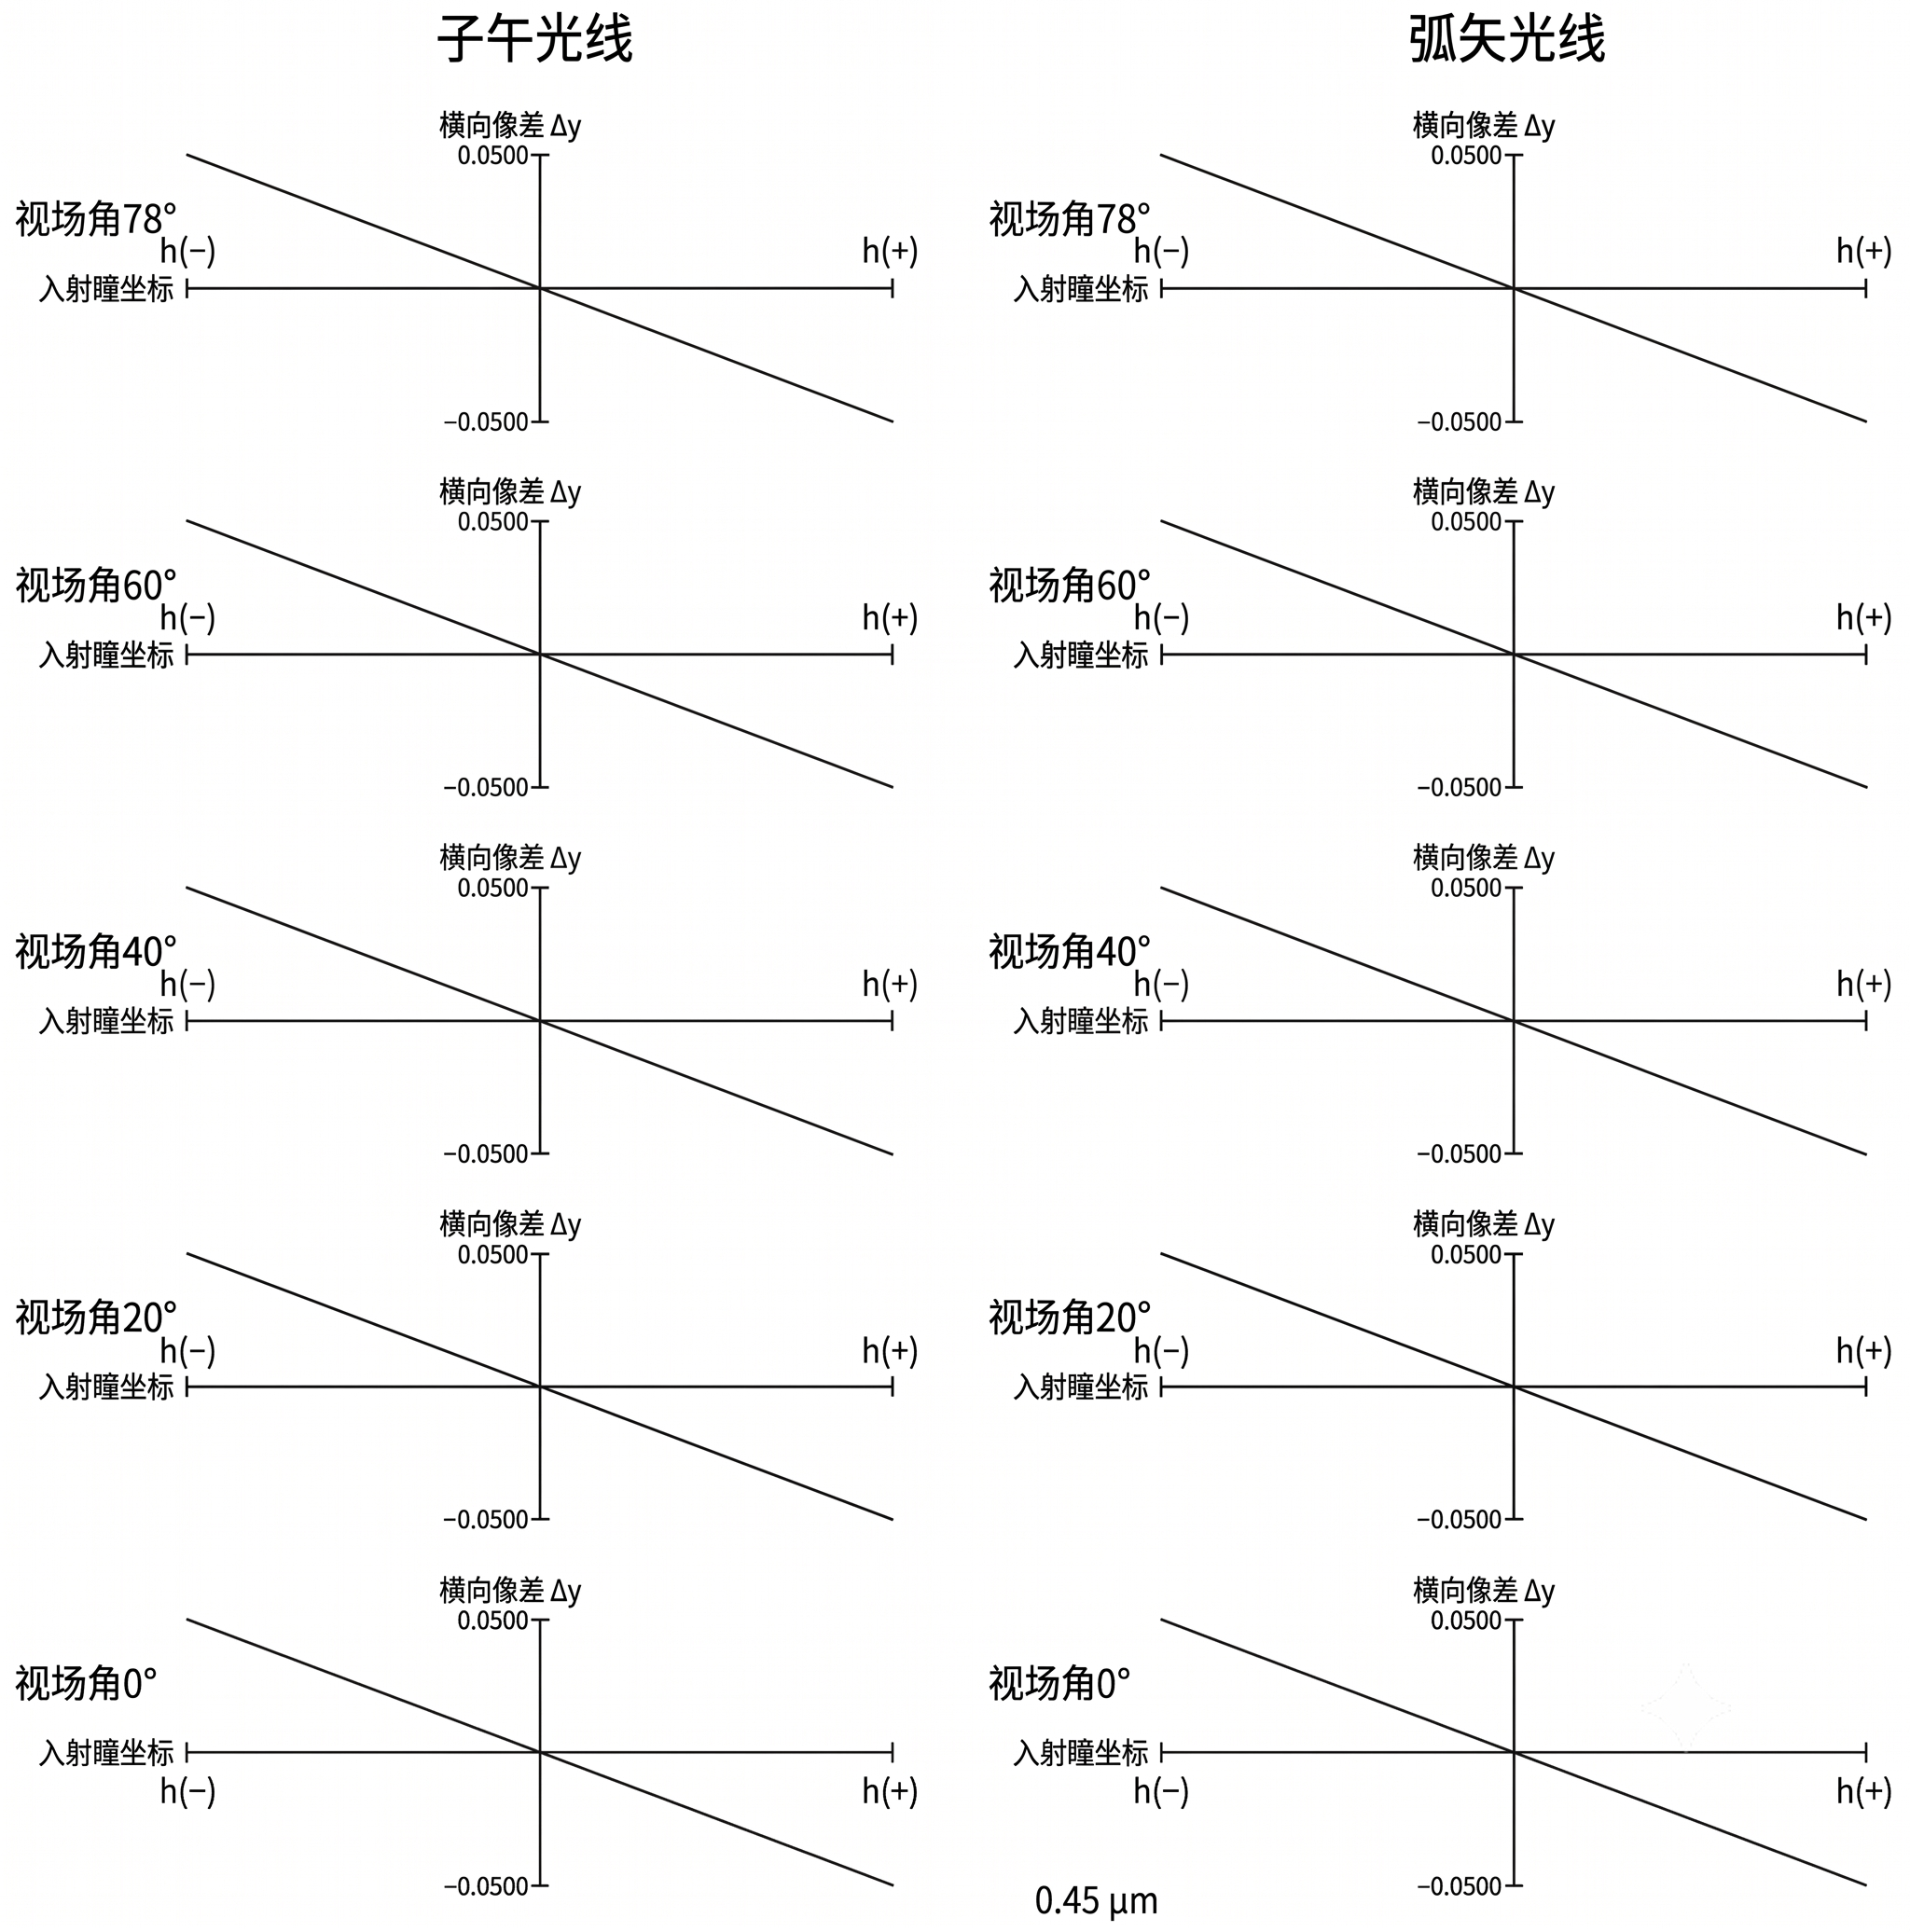
\includegraphics[width=.32\textwidth,height=.25\textheight,keepaspectratio]{Figure/图片20.png}\hfill
                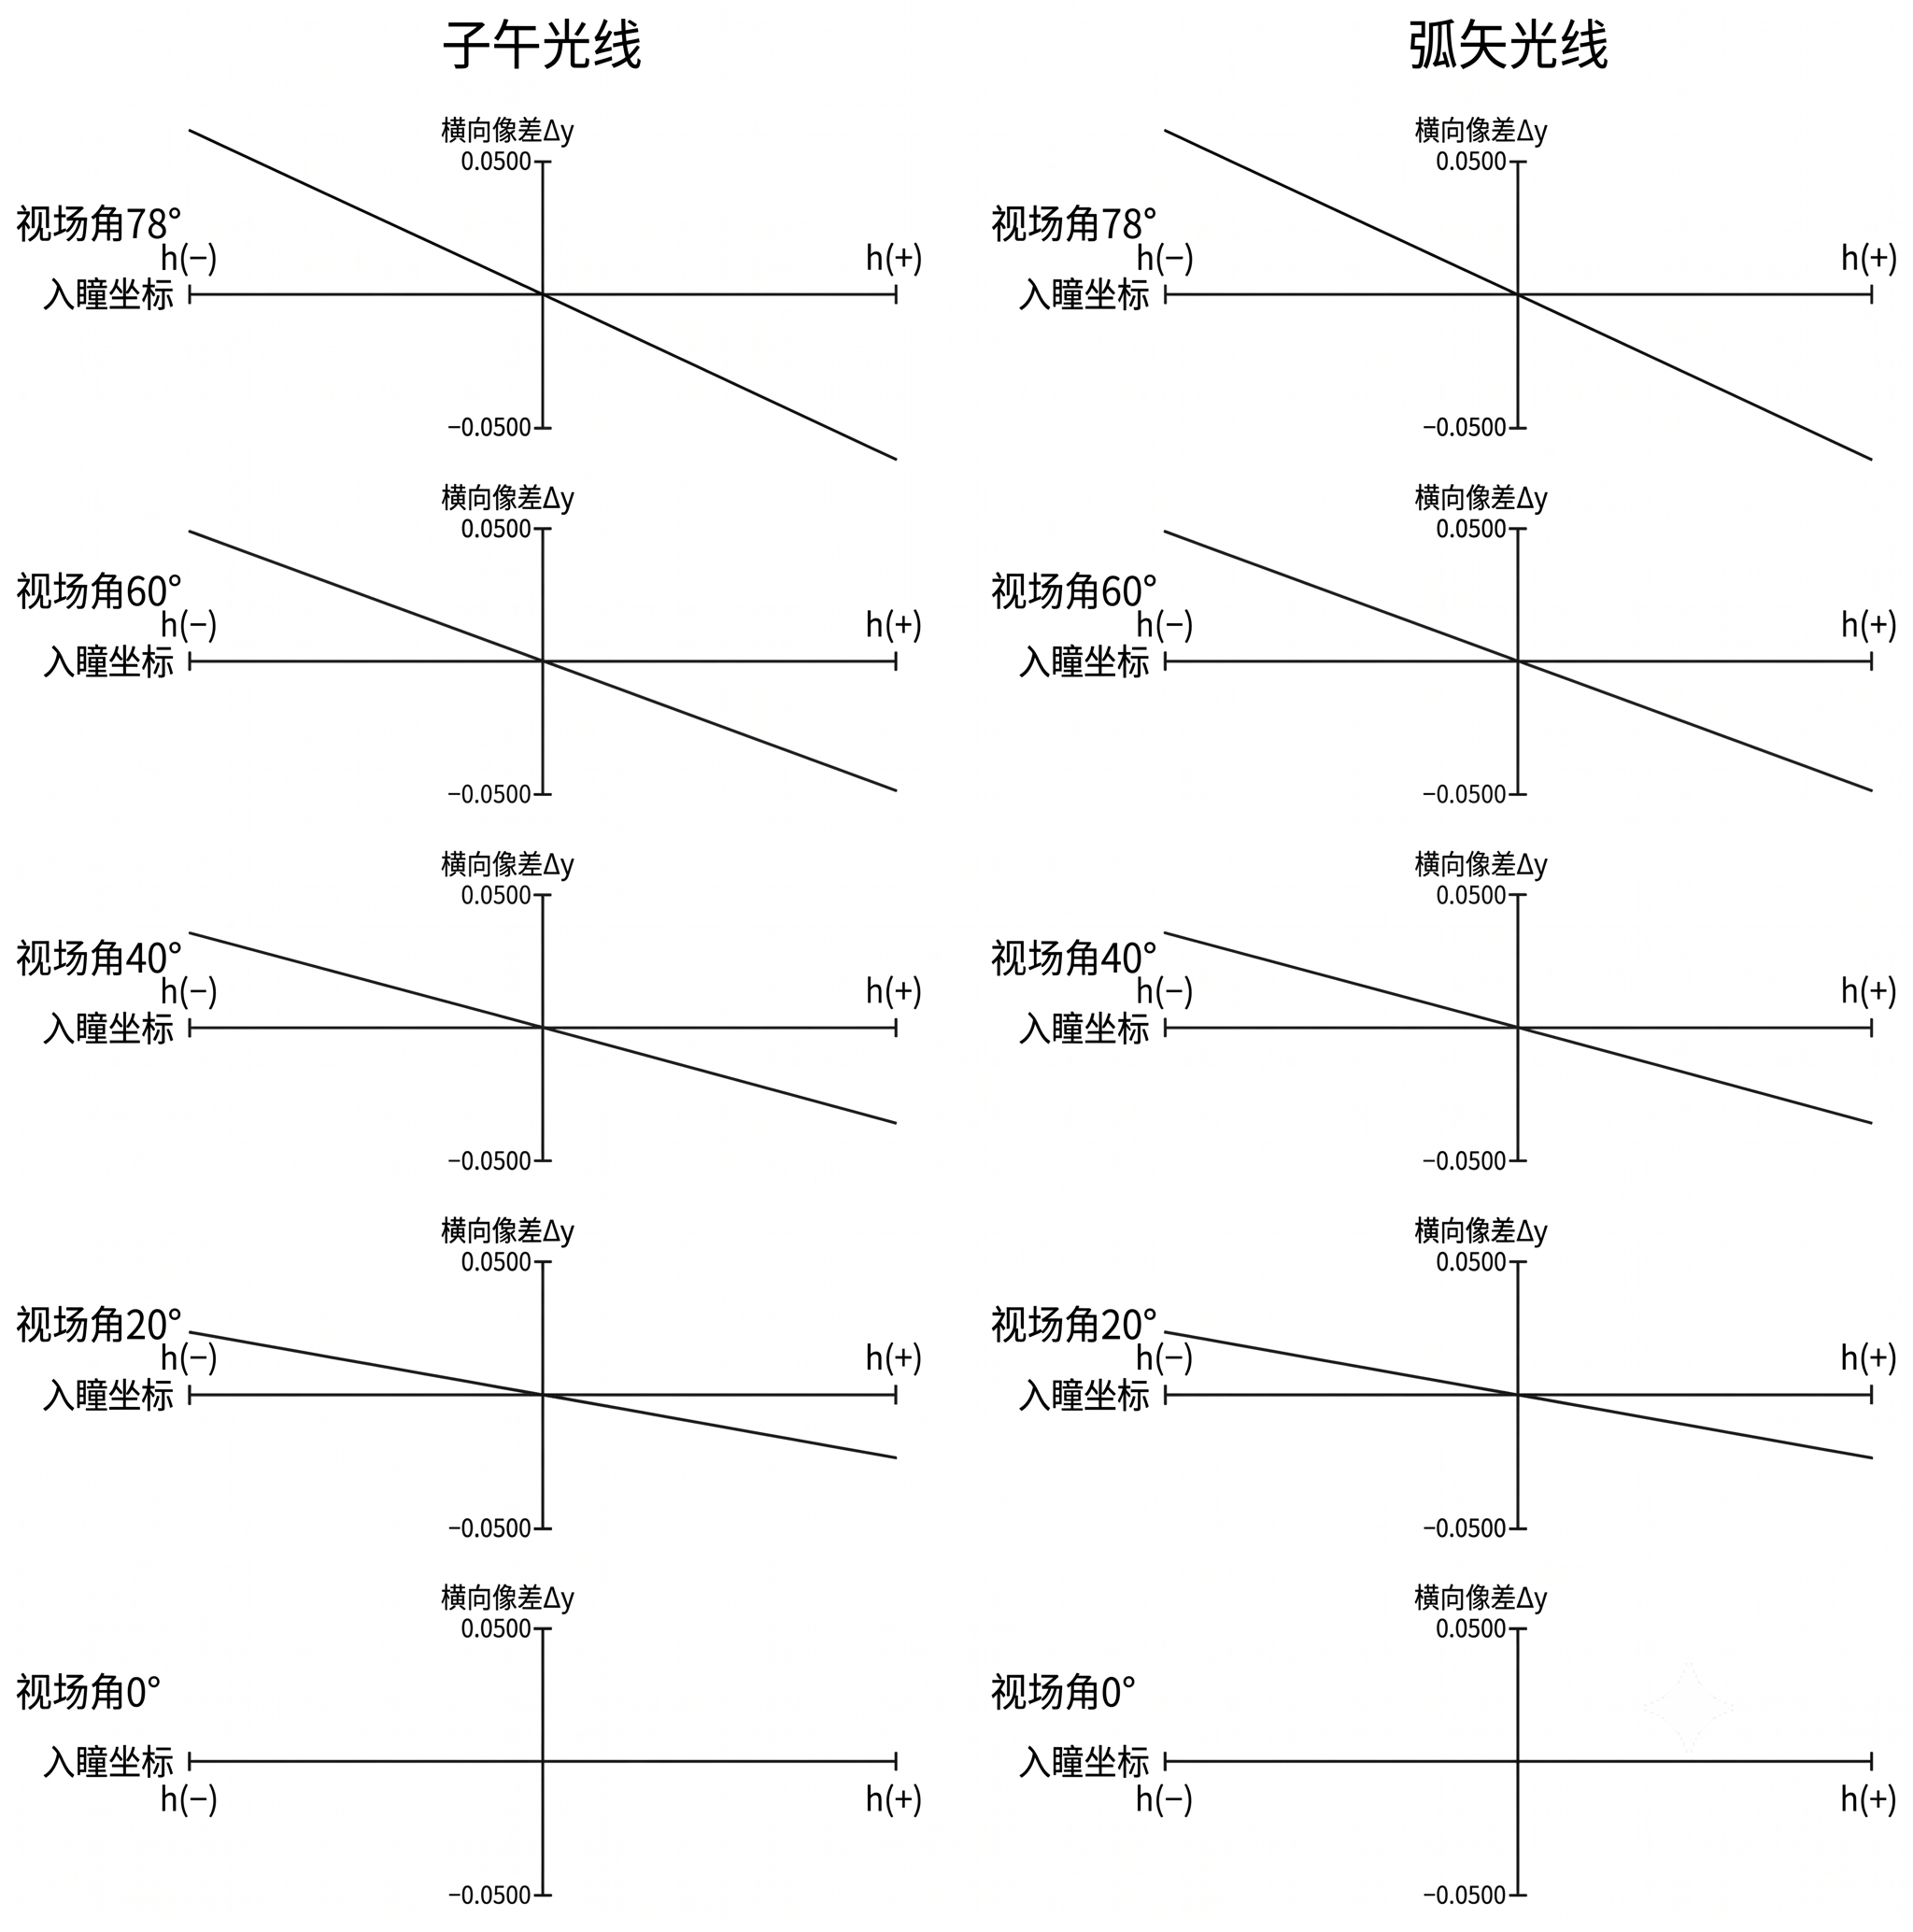
\includegraphics[width=.32\textwidth,height=.25\textheight,keepaspectratio]{Figure/图片21.png}\hfill
                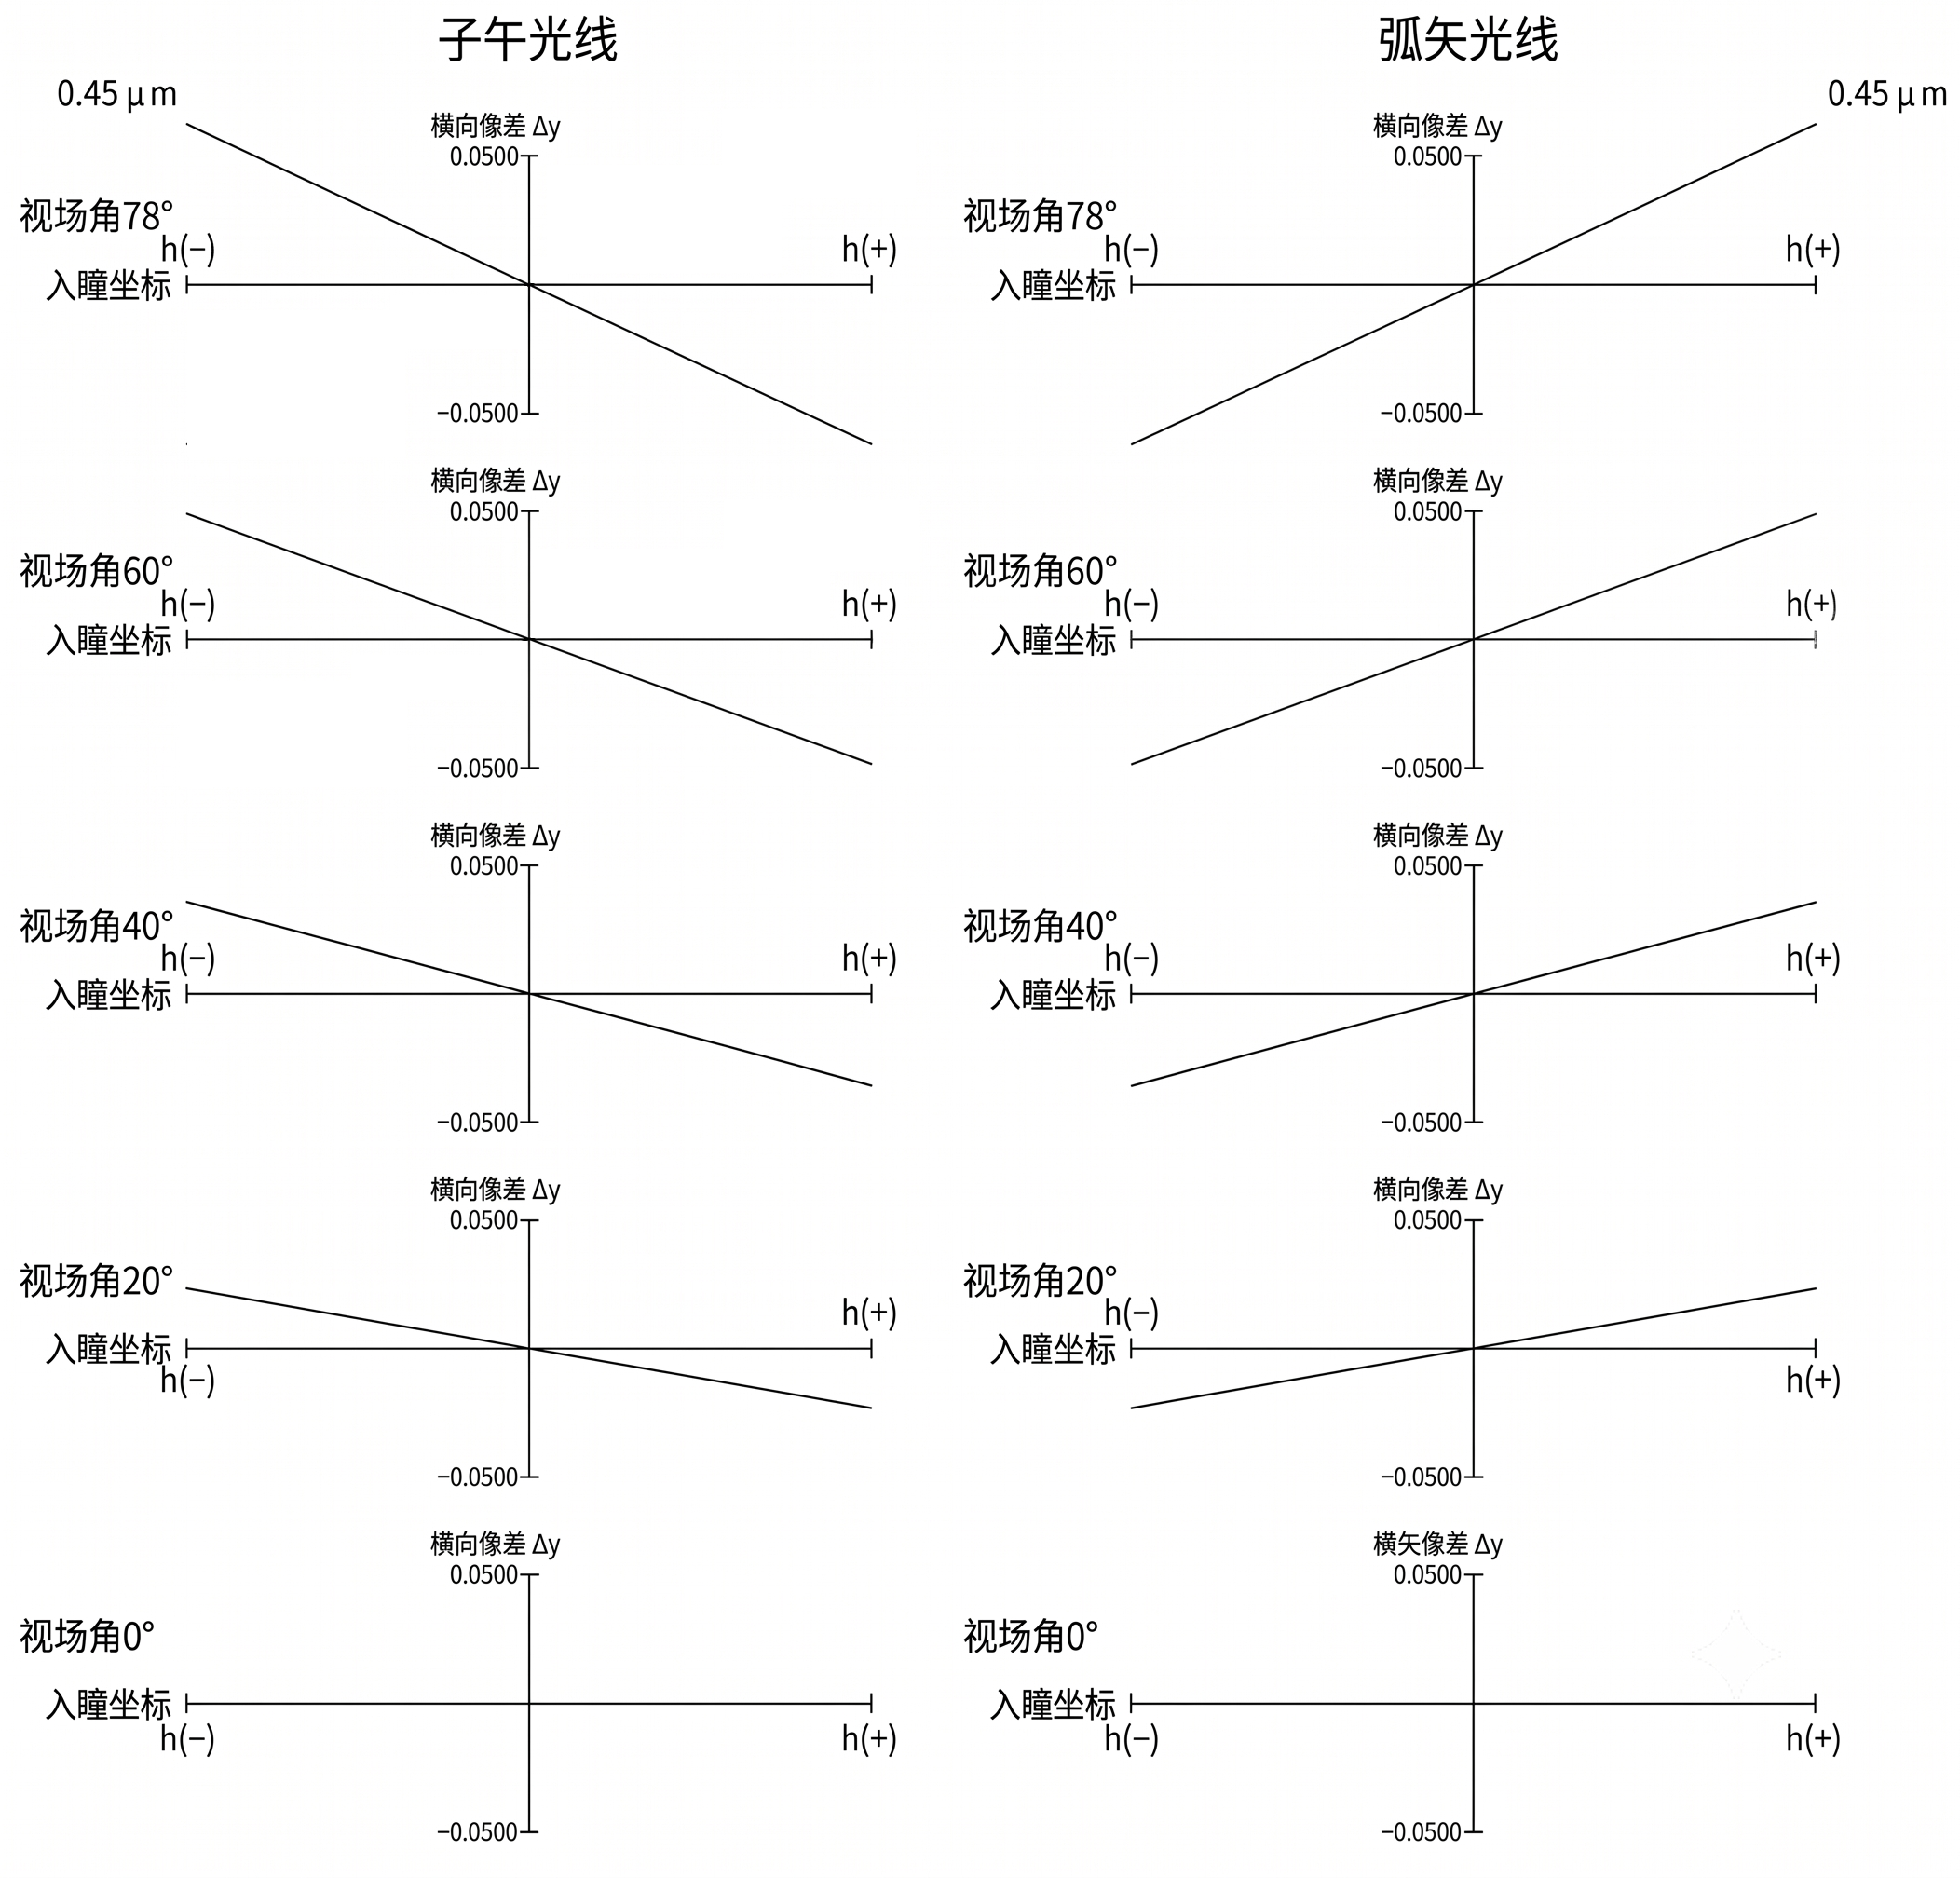
\includegraphics[width=.32\textwidth,height=.25\textheight,keepaspectratio]{Figure/图片22.png}
                \vspace{3pt}
                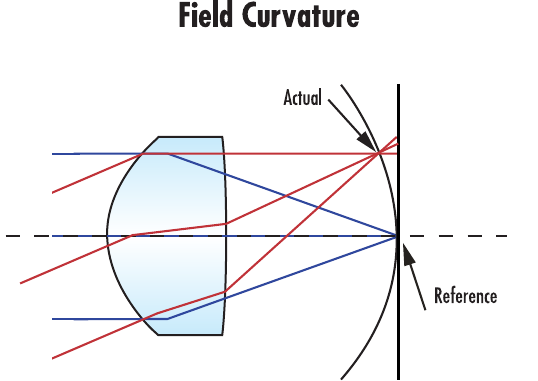
\includegraphics[width=\textwidth,height=.24\textheight,keepaspectratio]{Figure/Edmund/aberrations-4v2.png}
                \caption{上：离焦、场曲、像散的 Ray Fan；下：场曲的弯曲最佳像面}
                \label{fig:linear_field_curvature_main}
            \end{figure}
        \end{column}
        \hfill
        \begin{column}{.47\textwidth}
            \begin{block}{场曲}
                不同视场的最佳焦点落在不同轴向位置，本质上由 Petzval 和决定；移动平面探测器只能在中心和边缘之间折中。
            \end{block}

            \begin{block}{像散}
                子午与弧矢两组光线的最佳焦点分离，因此同一点物会先后形成两条正交焦线，中间只是最小弥散圆。
            \end{block}

            \begin{alertblock}{诊断顺序}
                先看不同视场的最佳焦点是否移动，再看 Tangential/Sagittal 两条曲线是否分离。
            \end{alertblock}
        \end{column}
    \end{columns}
\end{frame}

\englishtitle{Meridional and Sagittal Planes}
\begin{frame}{子午/弧矢：像散诊断所需的两个切面}
\label{1.12}
    \begin{columns}[T]
        \begin{column}{.56\textwidth}
            \begin{figure}
                \centering
                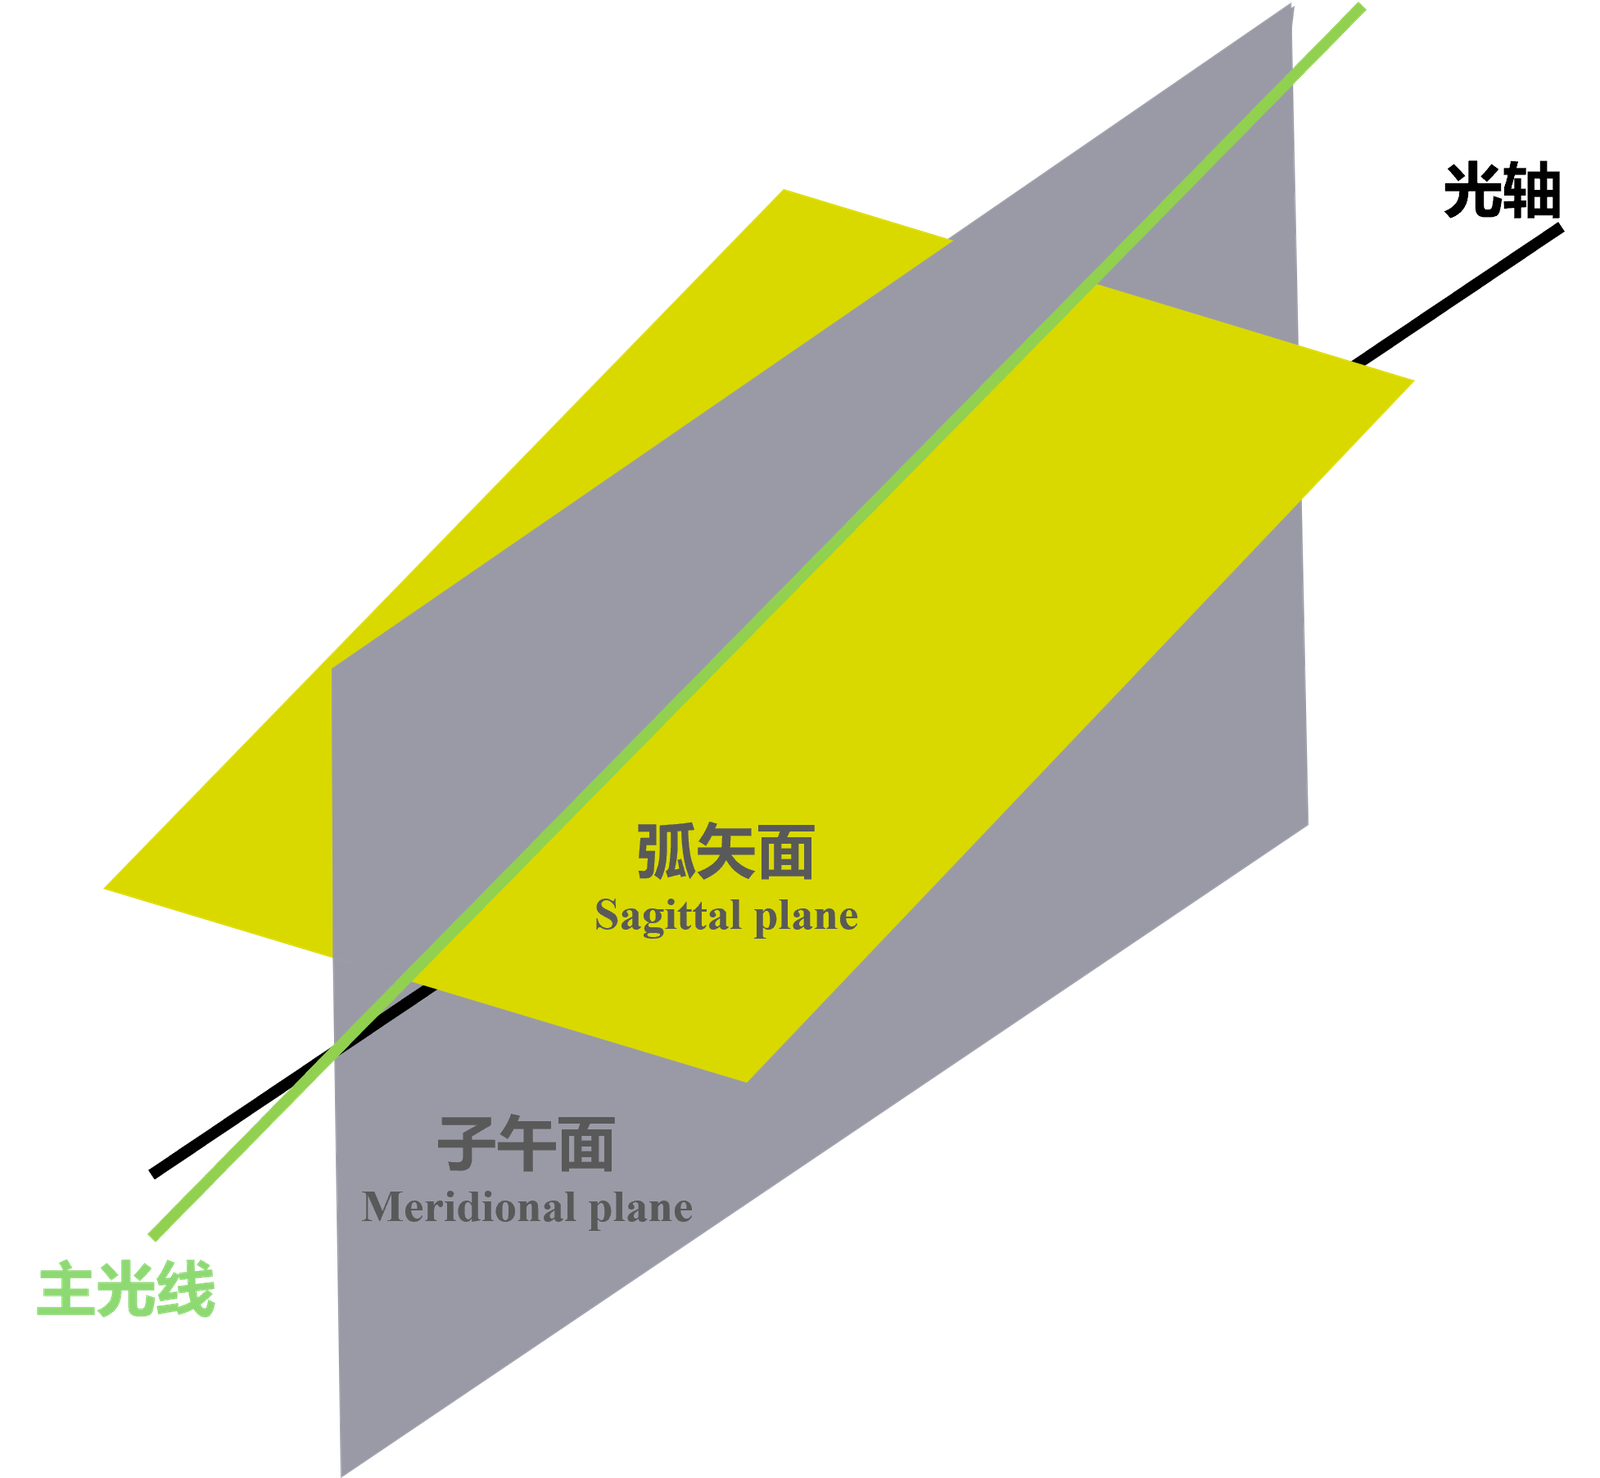
\includegraphics[width=.24\textwidth,height=.29\textheight,keepaspectratio]{Figure/图片18.png}\hfill
                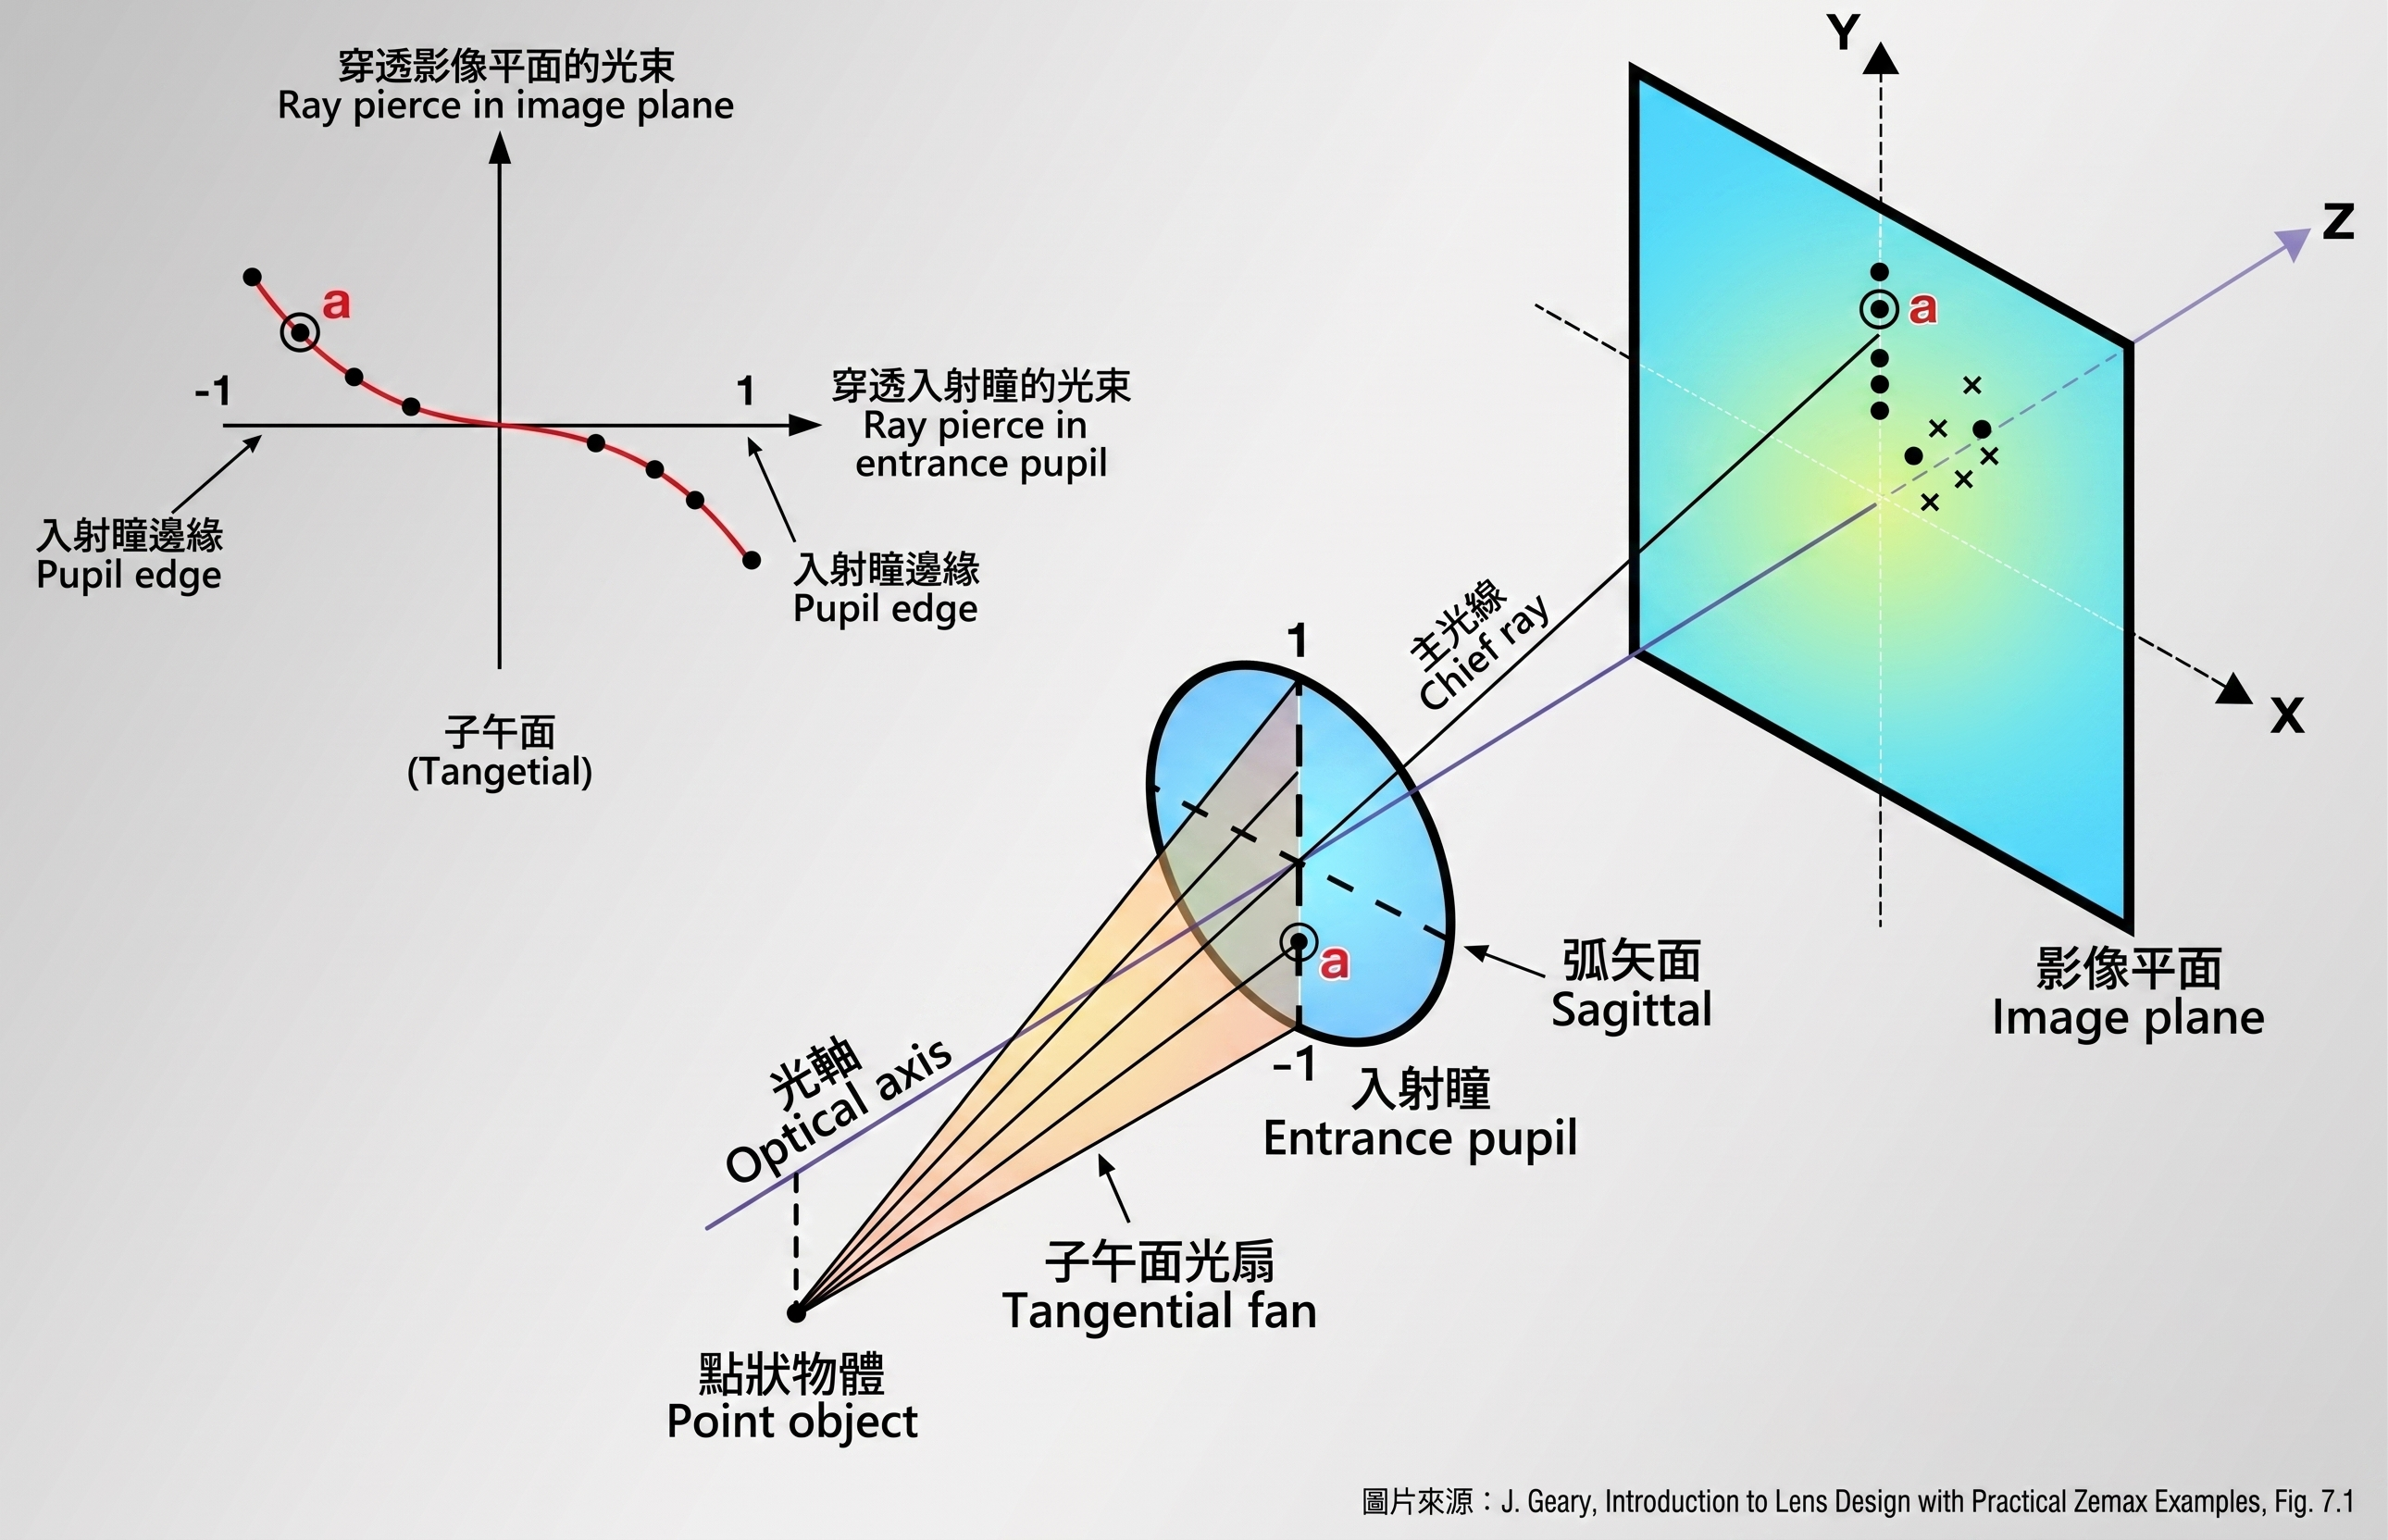
\includegraphics[width=.72\textwidth,height=.29\textheight,keepaspectratio]{Figure/图片26.png}
                \vspace{3pt}
                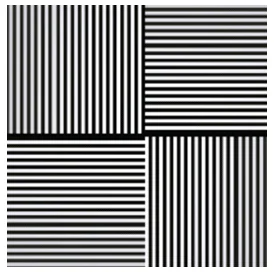
\includegraphics[width=.46\textwidth,height=.18\textheight,keepaspectratio]{Figure/Edmund/abberations-2a.png}\hfill
                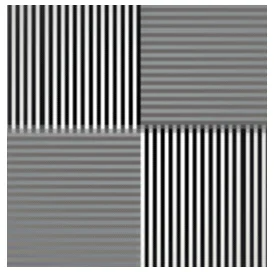
\includegraphics[width=.46\textwidth,height=.18\textheight,keepaspectratio]{Figure/Edmund/abberations-2b.png}
                \caption{上：子午面与弧矢面；下：像散导致两个方向不能同时清晰}
                \label{fig:meridional_sagittal_astigmatism_main}
            \end{figure}
        \end{column}
        \hfill
        \begin{column}{.44\textwidth}
            \begin{itemize}
                \item \textbf{子午面}包含光轴和主光线。
                \item \textbf{弧矢面}与子午面正交，并同样经过主光线。
                \item Zemax 的 Tangential Fan / Sagittal Fan，就是分别在这两个切面里观察 Ray Fan。
                \item 若只靠整体移动像面，通常只能在两条焦线之间折中，不能真正消掉像散。
            \end{itemize}

            \begin{block}{工程处理}
                常见手段包括弯月透镜、对称结构、调整光阑位置或降低离轴会聚角。
            \end{block}
        \end{column}
    \end{columns}
\end{frame}

\subsection{色散、阿贝图与玻璃选择}
\label{sec:1.5}

\englishtitle{Abbe Diagram and Chromatic Correction}
\begin{frame}{阿贝图：把色差问题落到材料选择}
\label{1.13}
    \begin{columns}[T]
        \begin{column}{.45\textwidth}
            \begin{figure}
                \centering
                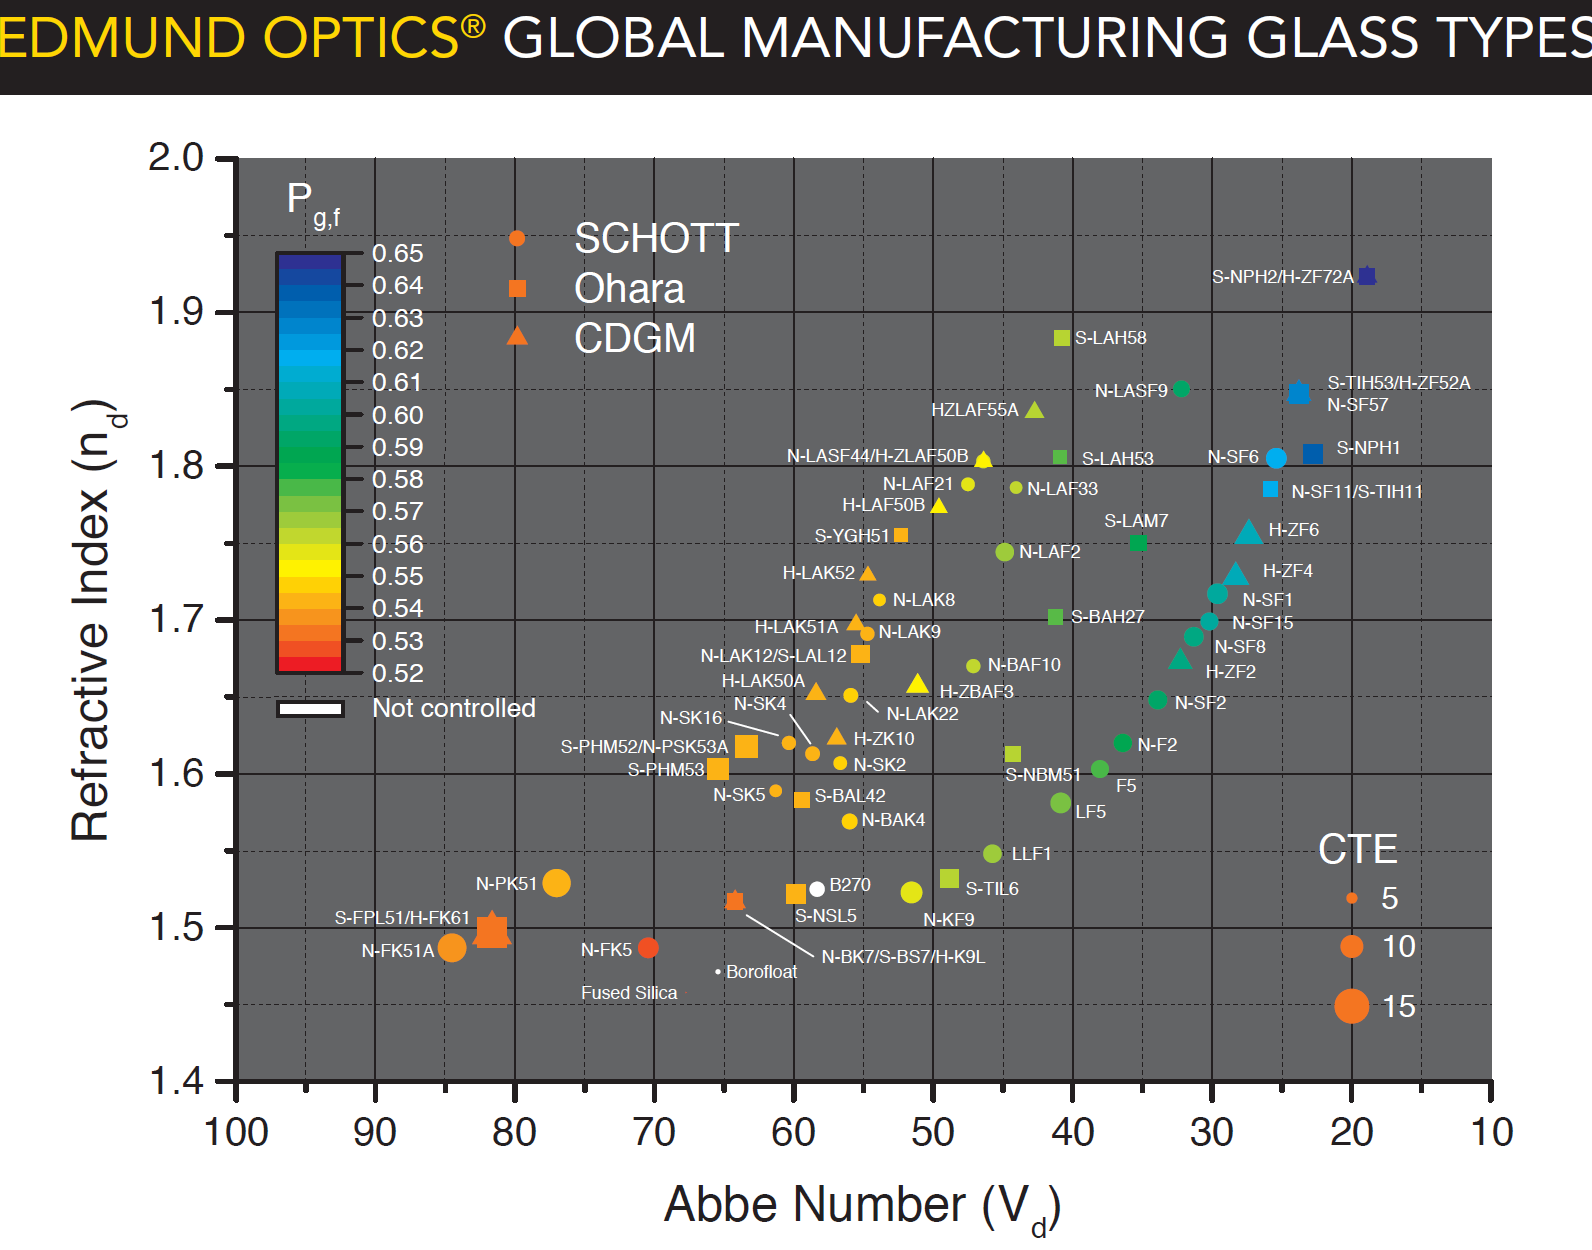
\includegraphics[width=.98\textwidth,height=.45\textheight,keepaspectratio]{Figure/Abbe.png}
                \caption{阿贝图：折射率与色散能力的材料地图}
                \label{fig:abbe_main}
            \end{figure}
        \end{column}
        \hfill
        \begin{column}{.55\textwidth}
            \textbf{色散是材料属性：}
            \begin{equation}
                \nu_d = \frac{n_d-1}{n_F-n_C}
                \label{eq:abbe_main}
            \end{equation}

            \begin{itemize}
                \item 低色散冕牌玻璃和高色散火石玻璃组合，是消色差双胶合的基本思路。
                \item Achromat 通常先让两种代表波长共焦；Apochromat 进一步压低第三波长和二级光谱残差。
                \item 对显微物镜，色差校正等级会直接推高材料自由度、镜片数量和制造成本。
            \end{itemize}

            \begin{alertblock}{合并后的主线}
                色差不要和材料选择分开讲：先看阿贝图决定材料空间，再回到 Ray Fan/OPD 判断色差是否真的被压低。
            \end{alertblock}
        \end{column}
    \end{columns}
\end{frame}

\englishtitle{Chromatic Aberration in Ray Fan}
\begin{frame}{色差在 Ray Fan 上怎么看}
\label{1.14}
    \begin{columns}[T]
        \begin{column}{.50\textwidth}
            \begin{figure}
                \centering
                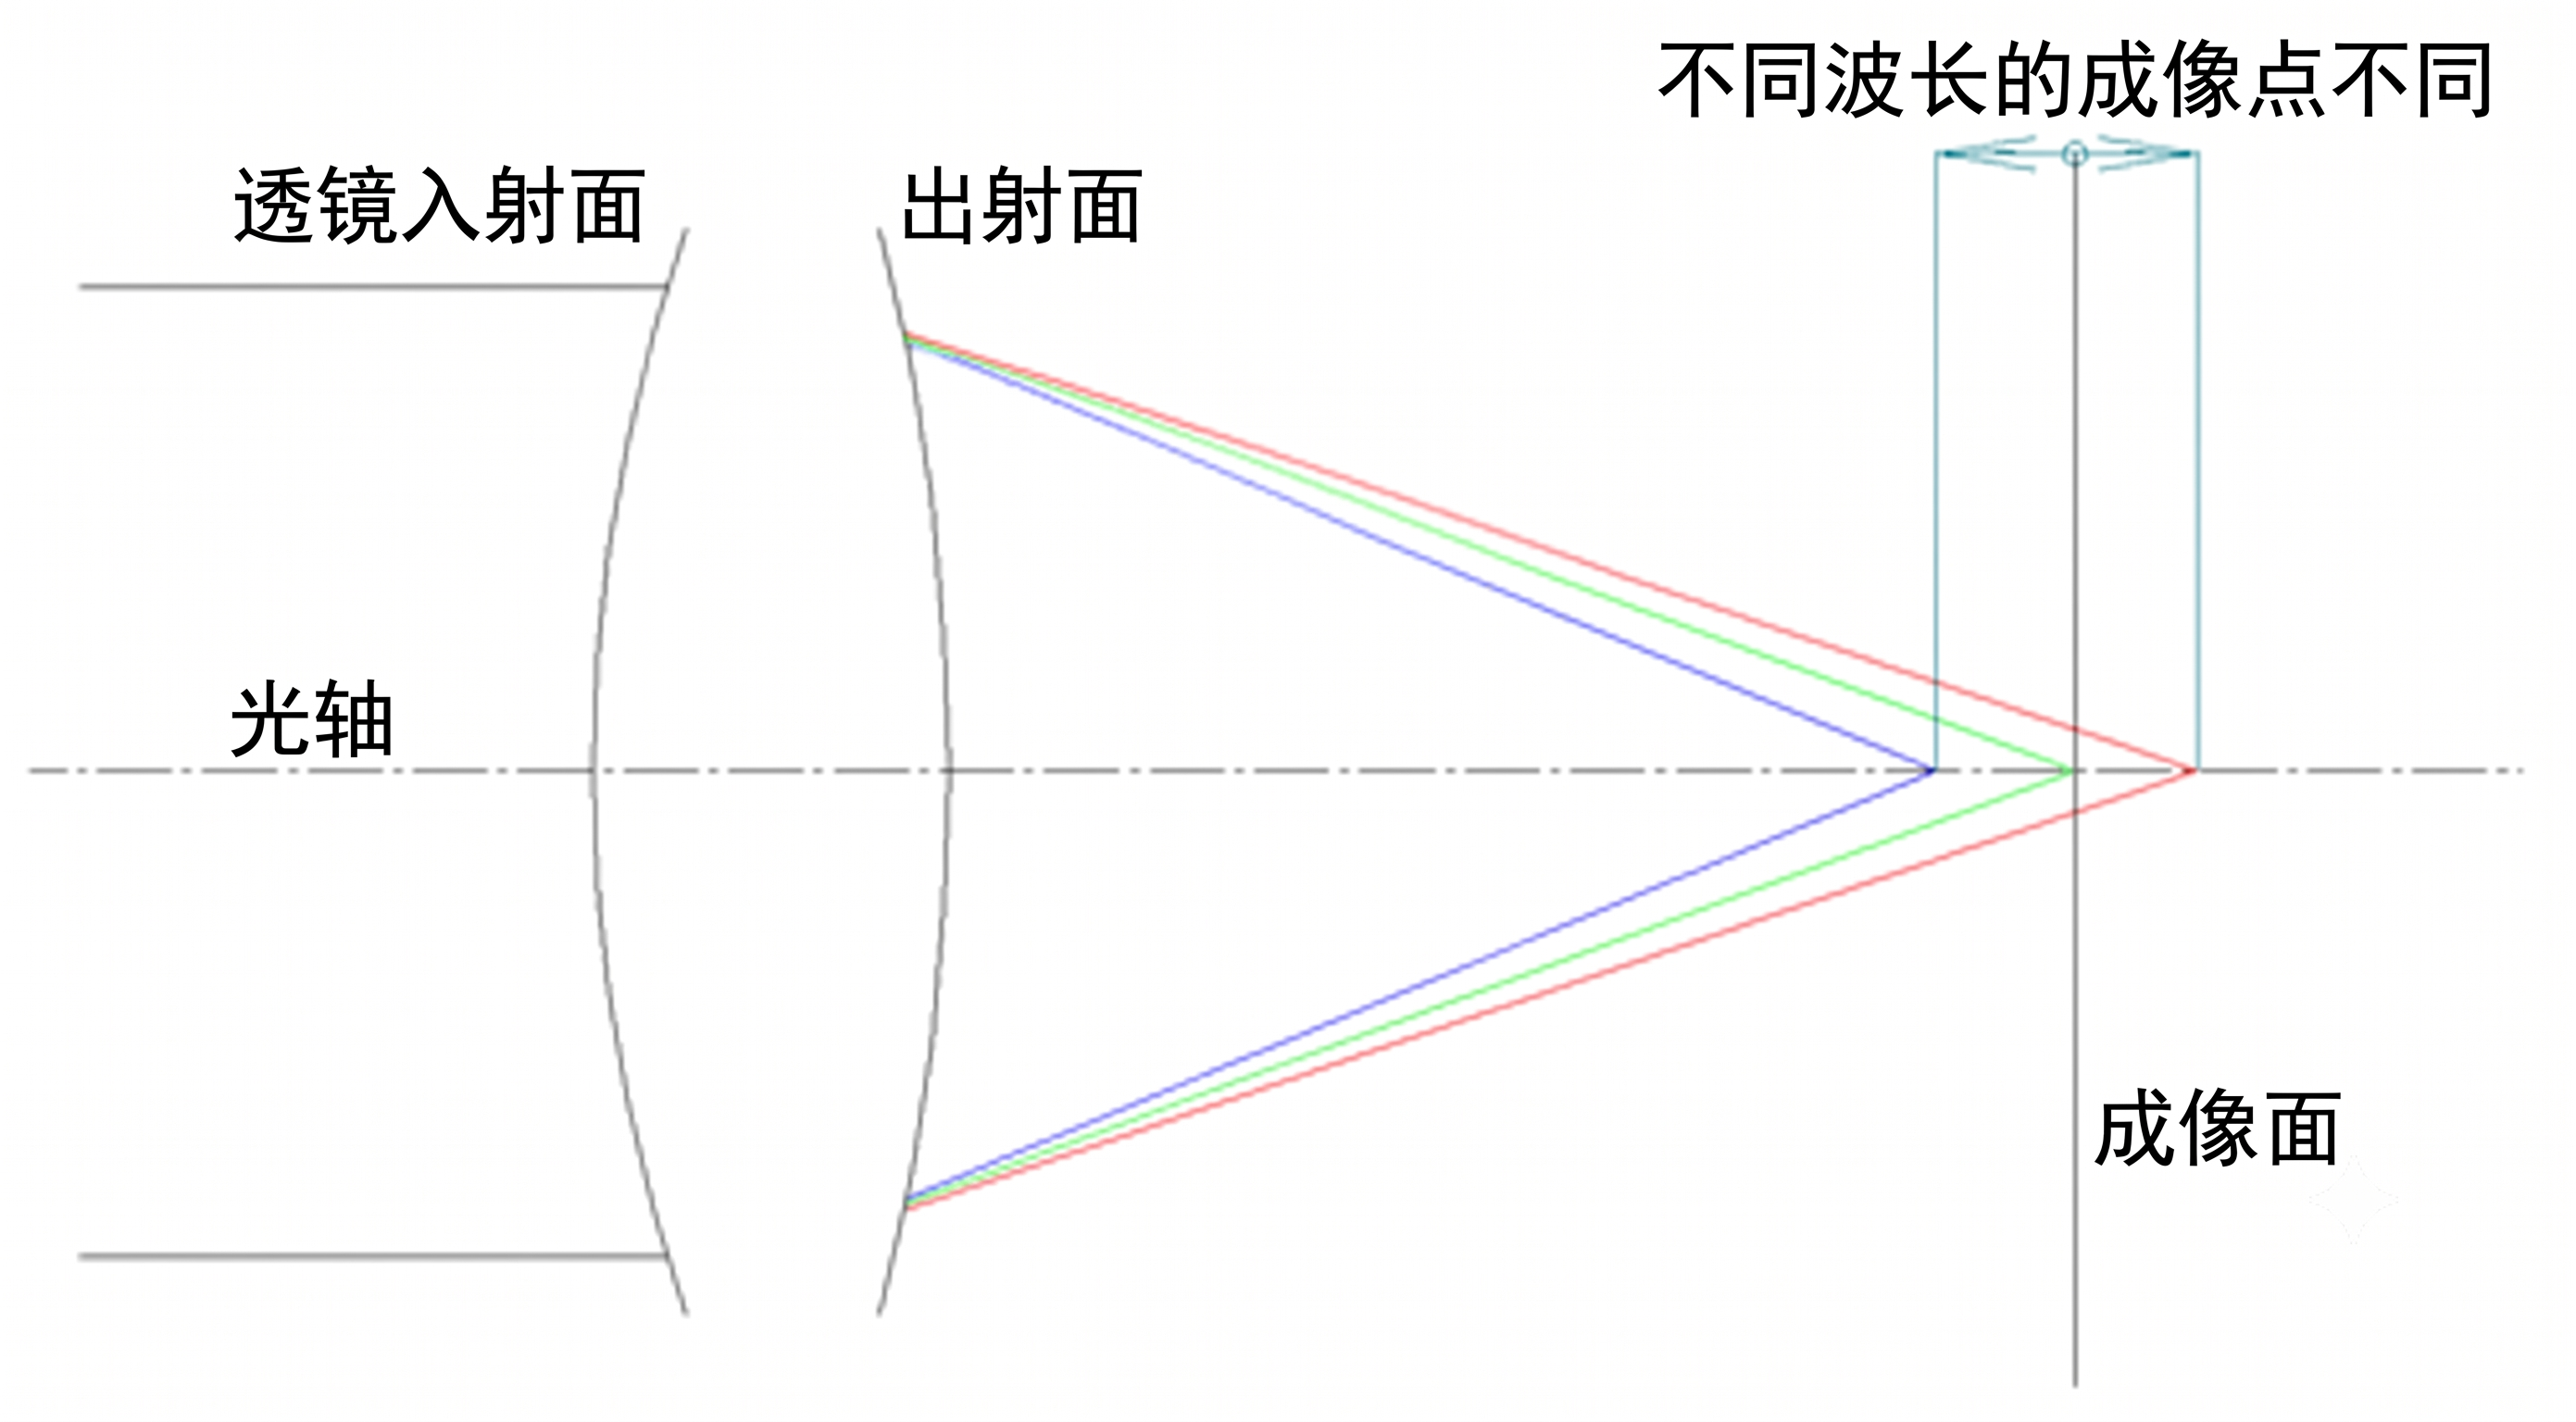
\includegraphics[width=.98\textwidth,height=.27\textheight,keepaspectratio]{Figure/图片30.png}
                \vspace{2pt}
                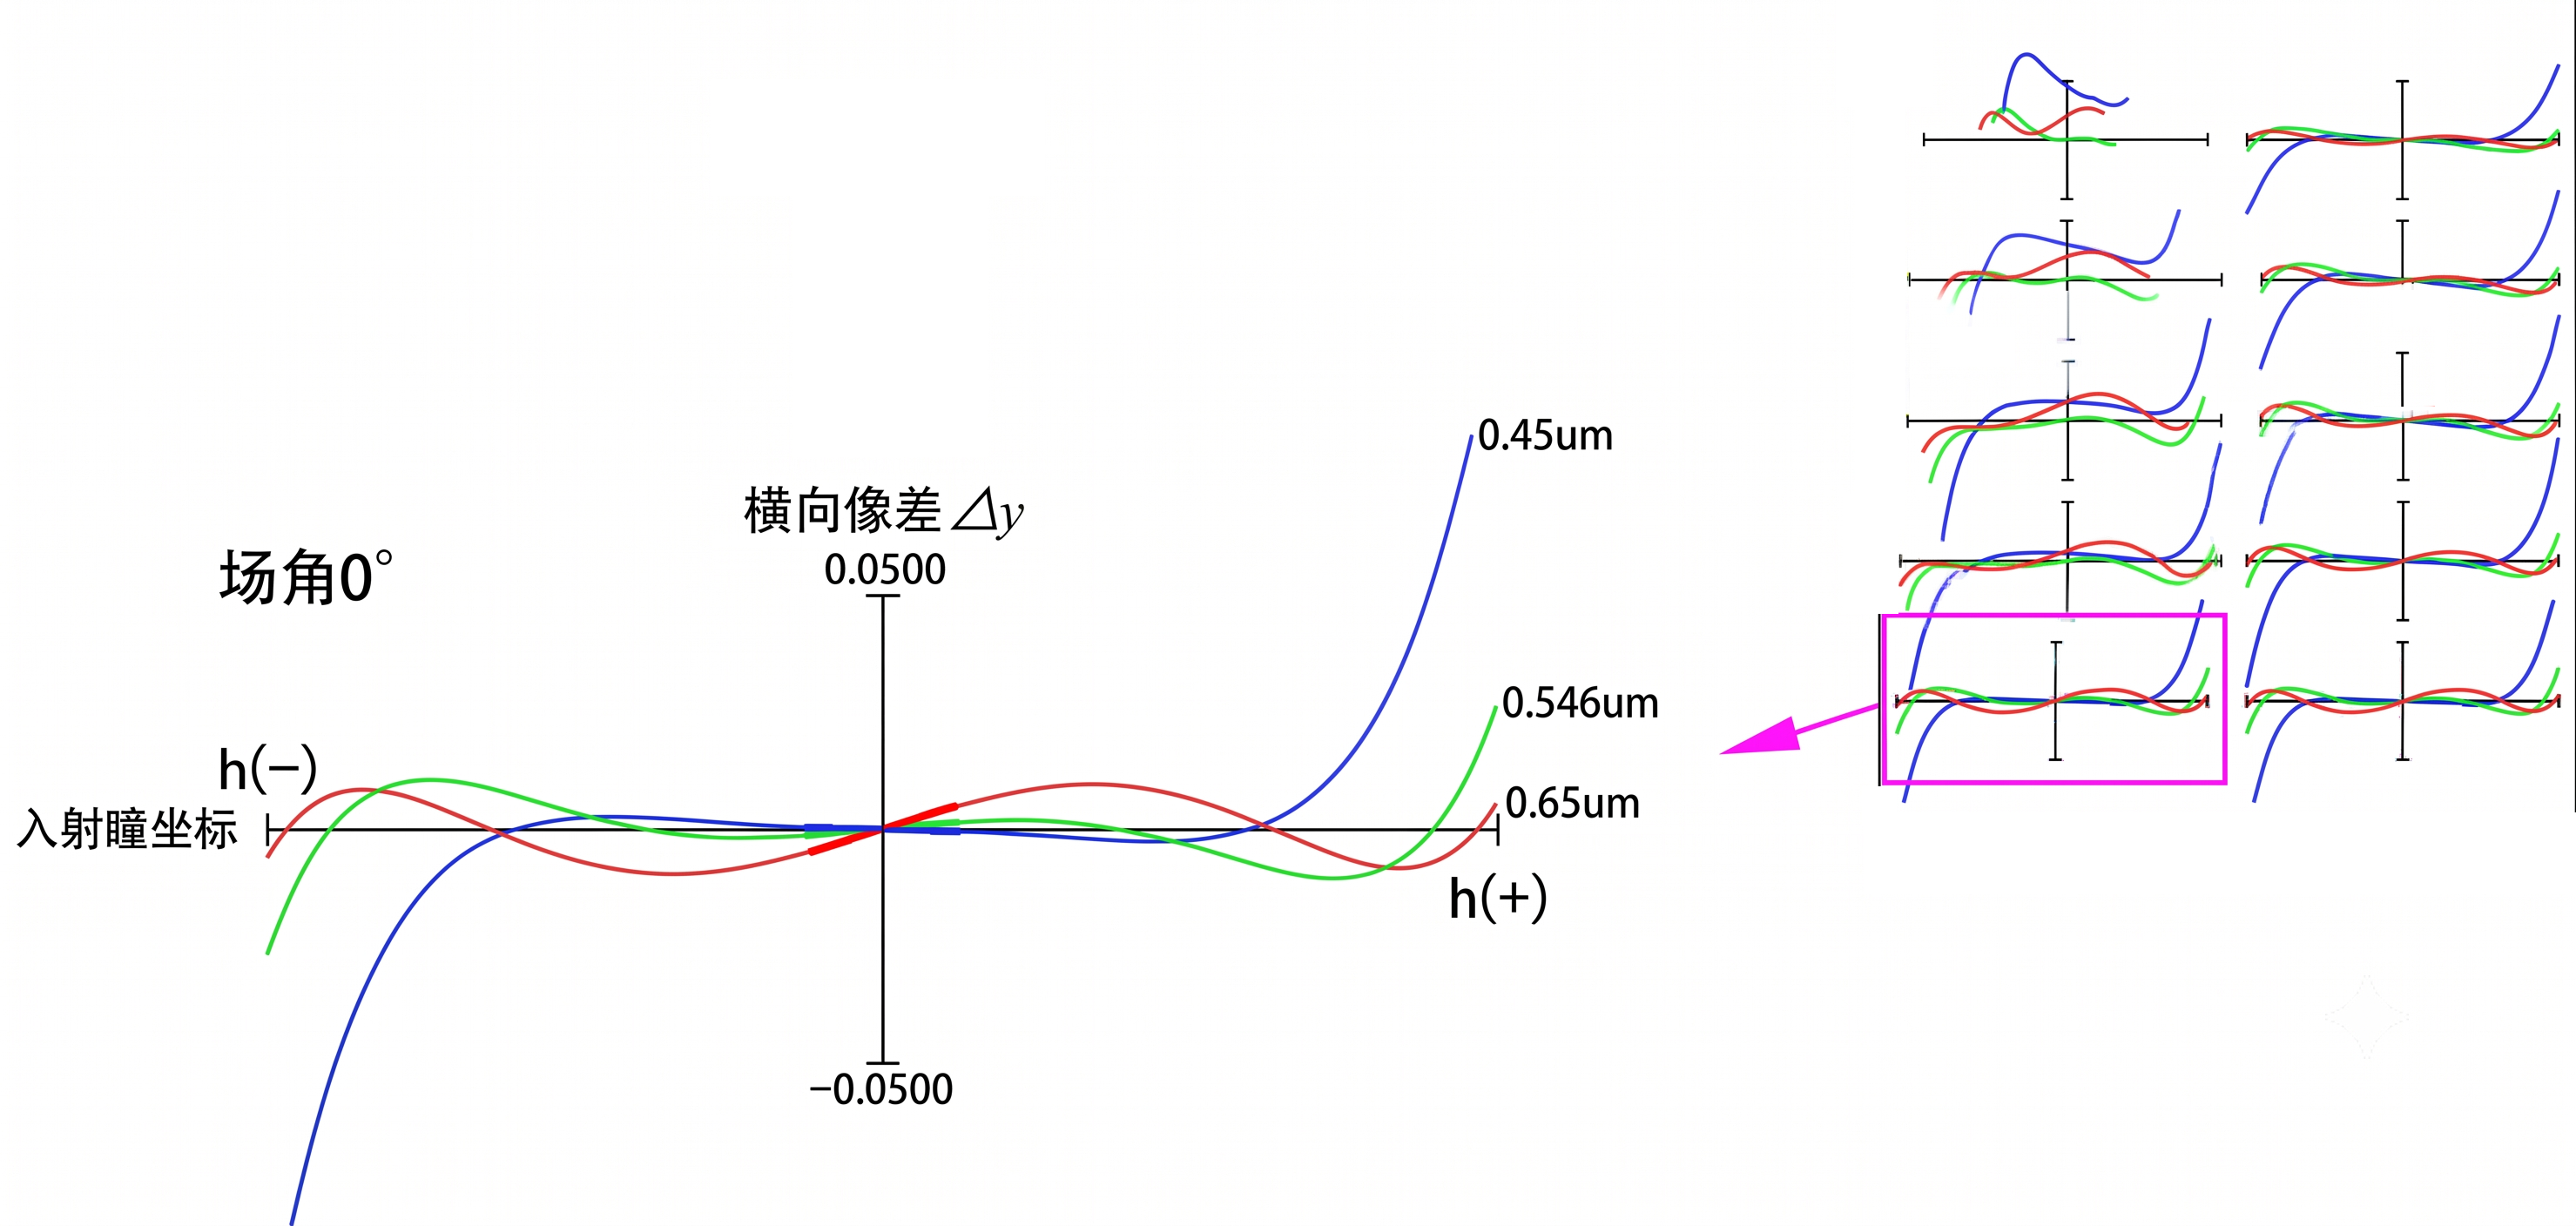
\includegraphics[width=.98\textwidth,height=.19\textheight,keepaspectratio]{Figure/图片28.png}
                \caption{轴向色差：不同波长近轴焦点位置不同}
                \label{fig:axial_color_main}
            \end{figure}
        \end{column}
        \hfill
        \begin{column}{.50\textwidth}
            \begin{figure}
                \centering
                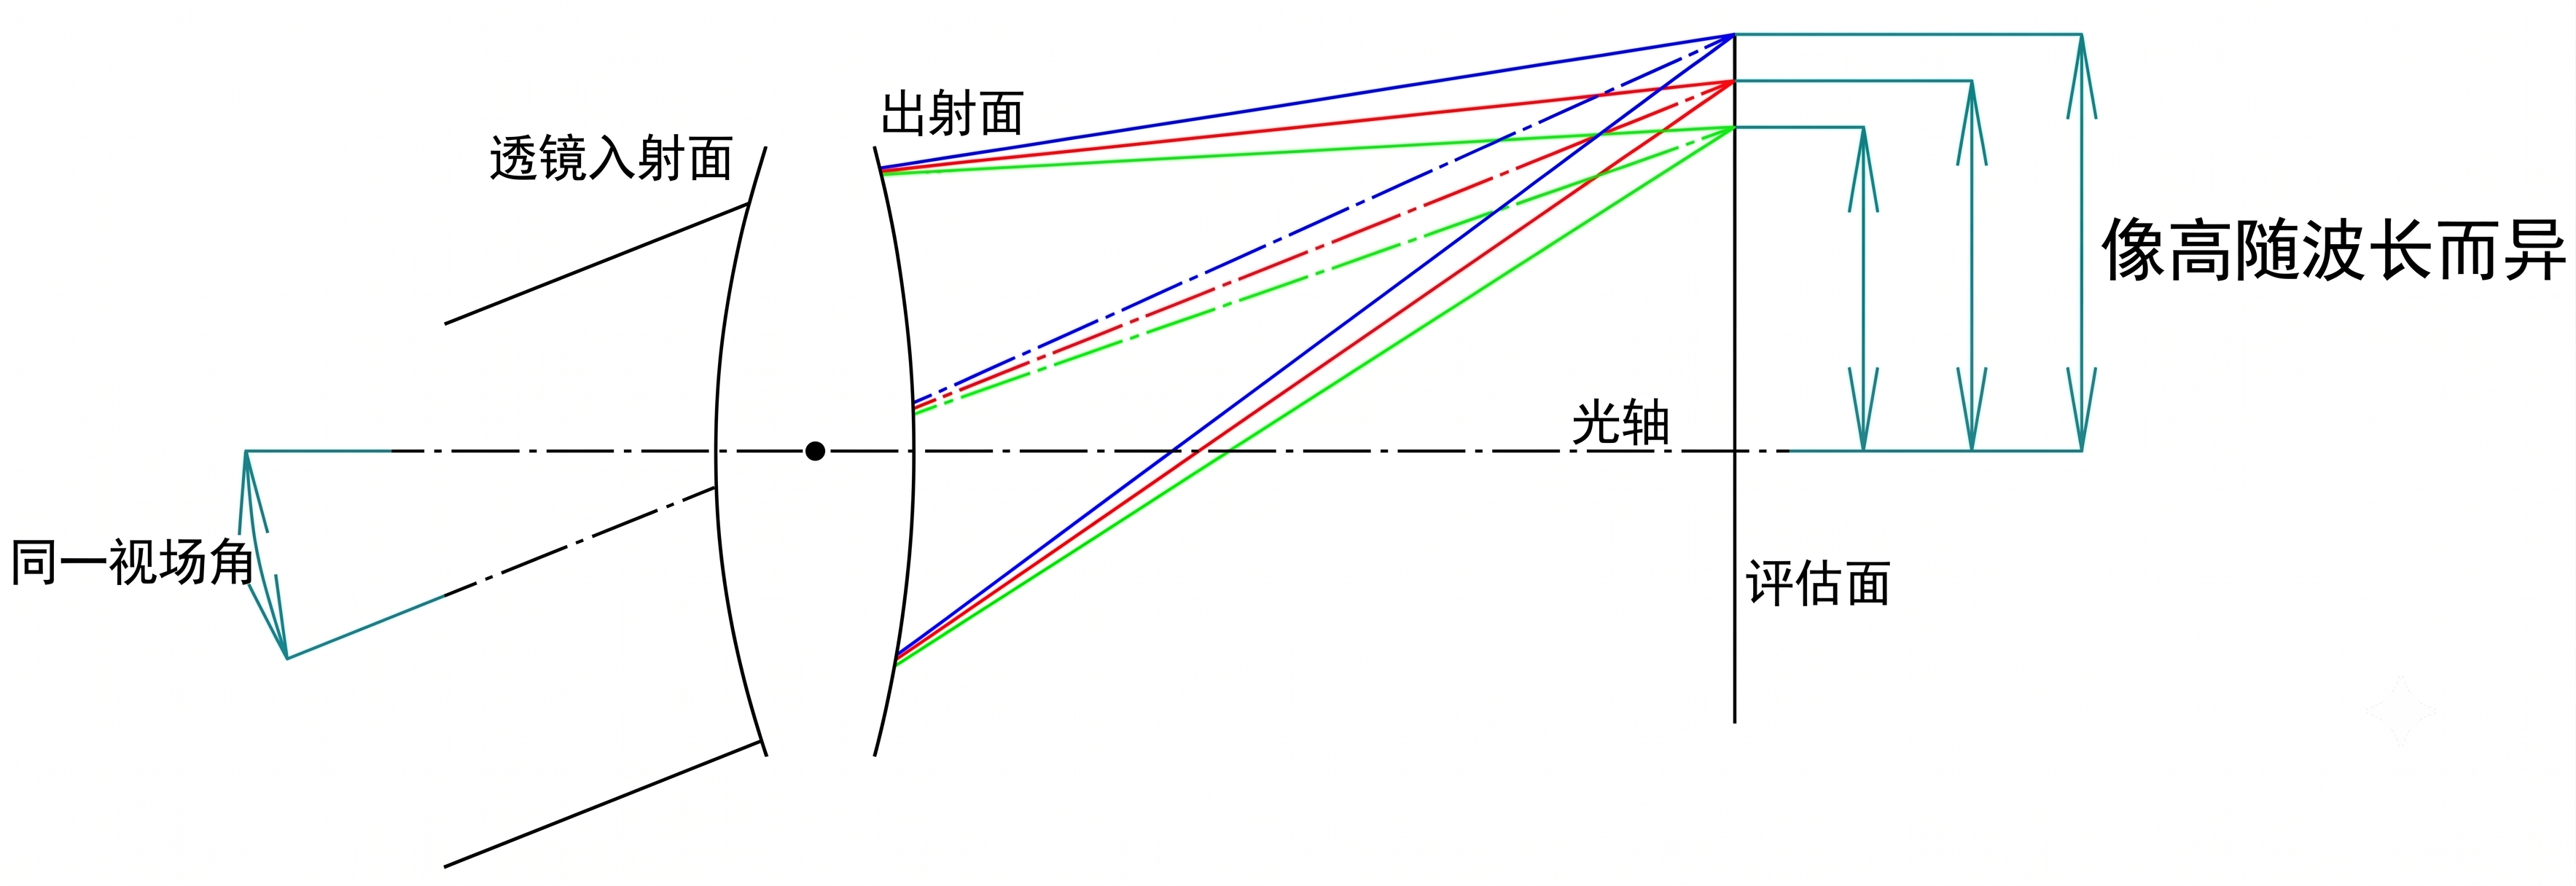
\includegraphics[width=.98\textwidth,height=.27\textheight,keepaspectratio]{Figure/图片31.png}
                \vspace{2pt}
                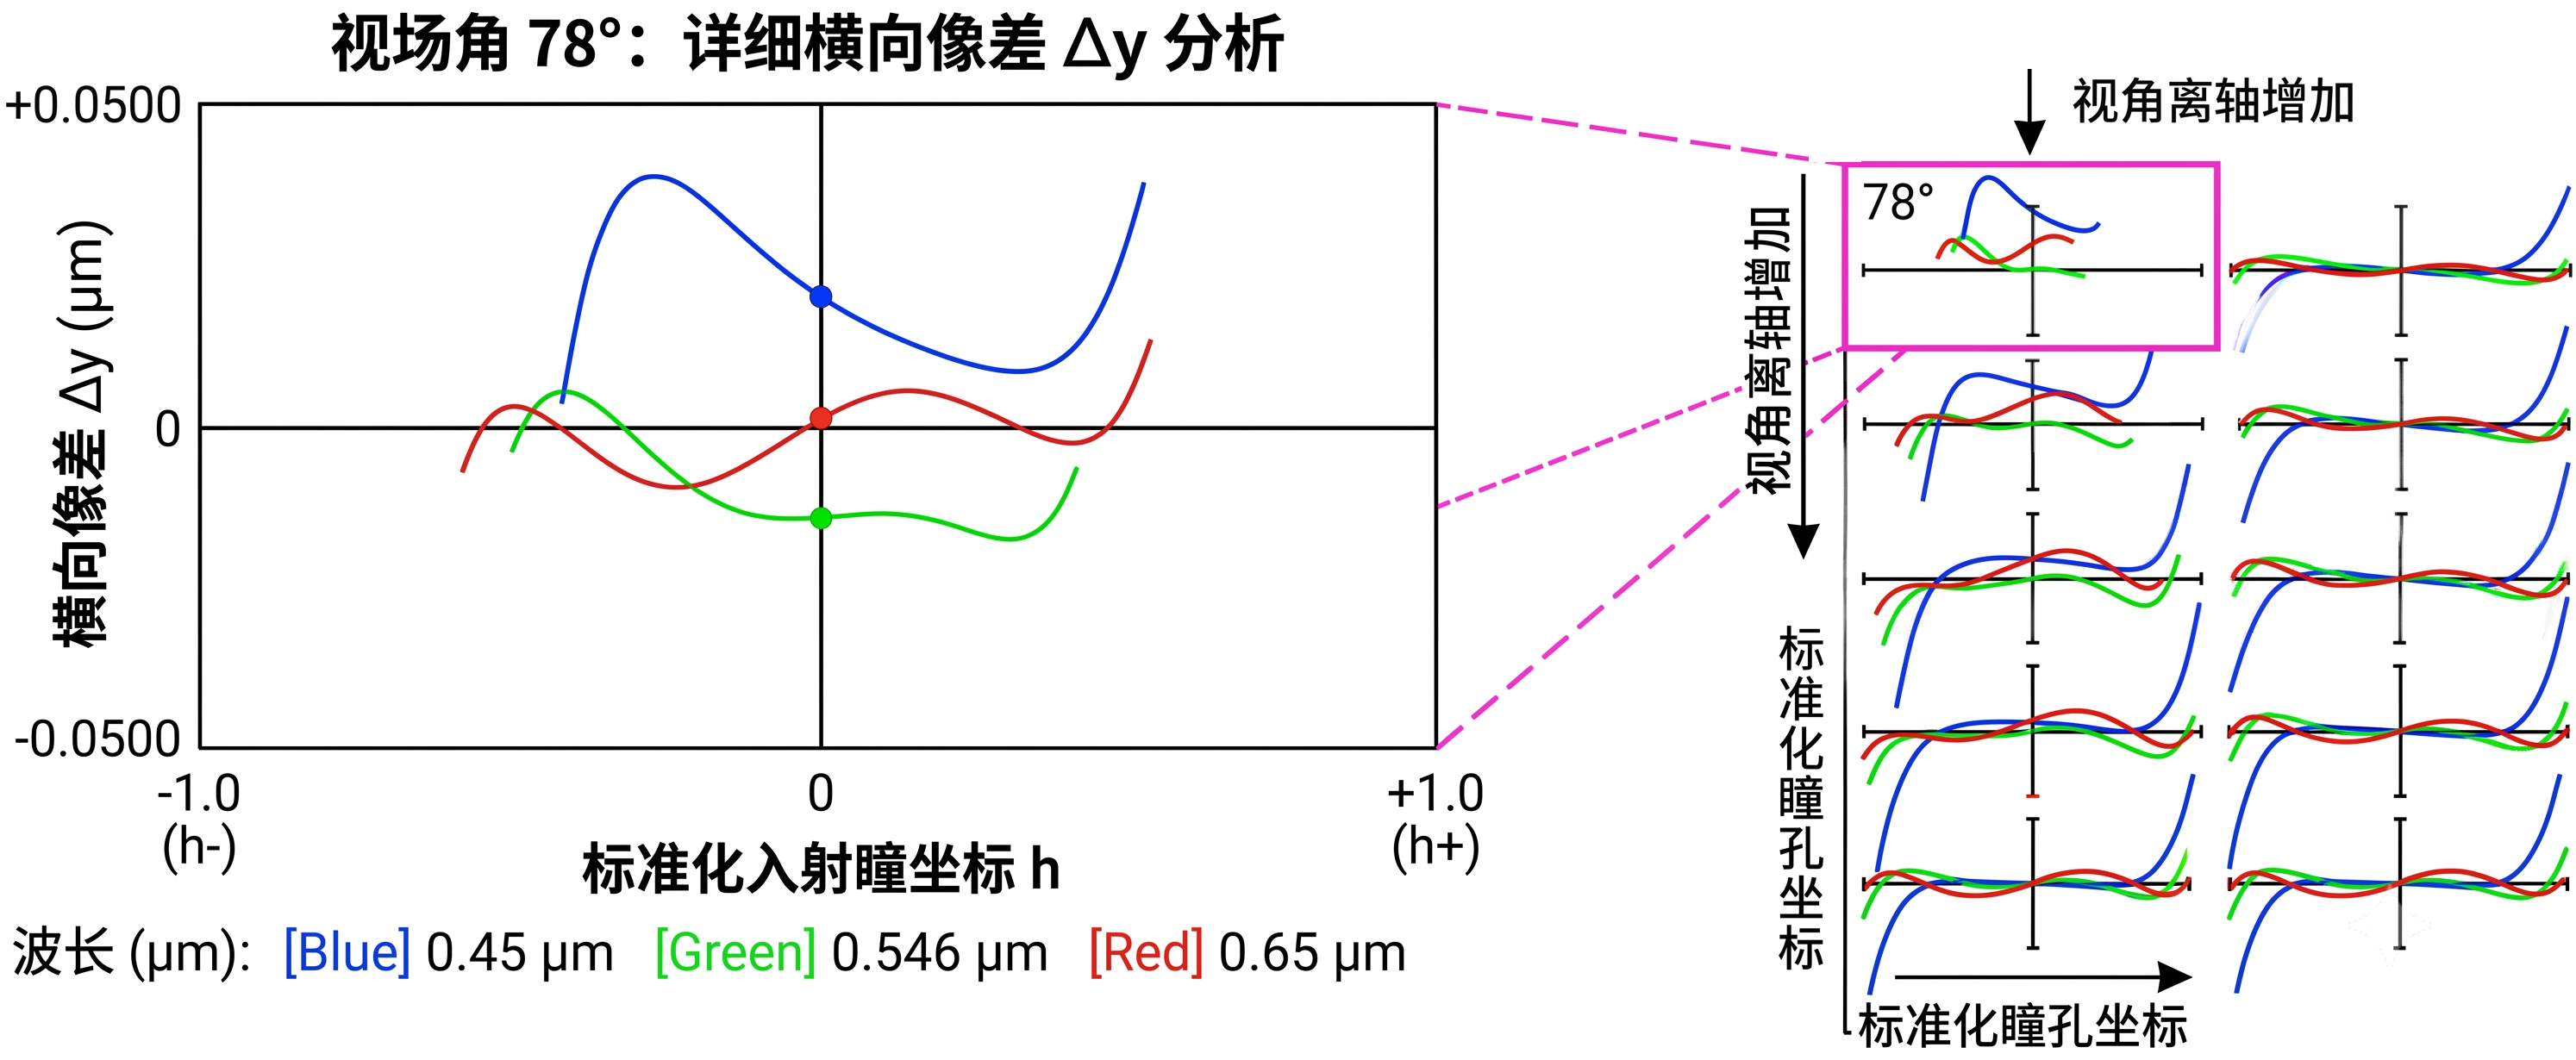
\includegraphics[width=.98\textwidth,height=.19\textheight,keepaspectratio]{Figure/图片29.png}
                \caption{倍率色差：不同波长主光线像高不同}
                \label{fig:lateral_color_main}
            \end{figure}
        \end{column}
    \end{columns}

    \vspace{-4pt}
    \begin{table}
        \centering
        \scriptsize
        \renewcommand{\arraystretch}{1.25}
        \begin{tabular}{p{2.0cm}|p{4.2cm}|p{4.2cm}}
            \toprule
            \textbf{类型} & \textbf{Ray Fan 特征} & \textbf{优化抓手} \\
            \midrule
            轴向色差 & 同一视场下，不同波长在原点附近斜率不同 & 玻璃组合、多波长权重、消色差约束 \\
            倍率色差 & 轴外视场中，不同波长主光线截距不同 & 对称结构、主光线色散控制、离轴波长权重 \\
            \bottomrule
        \end{tabular}
    \end{table}
\end{frame}

\englishtitle{Glass Substitution Workflow}
\begin{frame}{玻璃替换：直接在真实玻璃目录中优化}
\label{1.15}
    \begin{columns}[T]
        \begin{column}{.45\textwidth}
            \begin{enumerate}
                \item 在 LDE 中将玻璃 Solve 类型设为 \alert{Substitute}。
                \item 选择供应商目录，如 Schott、Hoya、Ohara、CDGM。
                \item 构建 RMS Wavefront 或 MTF/Spot 相关评价函数。
                \item 使用 Hammer 或 Global Search 处理离散玻璃变化。
                \item 用玻璃替换模板过滤成本、供应状态和耐候性。
            \end{enumerate}

            \begin{alertblock}{关键}
                玻璃型号是离散变量，Local Optimization 不擅长跨越材料跳变；全局搜索更适合玻璃替换。
            \end{alertblock}
        \end{column}
        \hfill
        \begin{column}{.55\textwidth}
            \begin{figure}
                \centering
                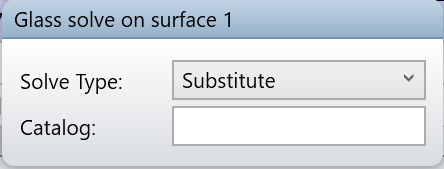
\includegraphics[width=.48\textwidth,height=.24\textheight,keepaspectratio]{Figure/玻璃替换/Picture1zh-cn.png}\hfill
                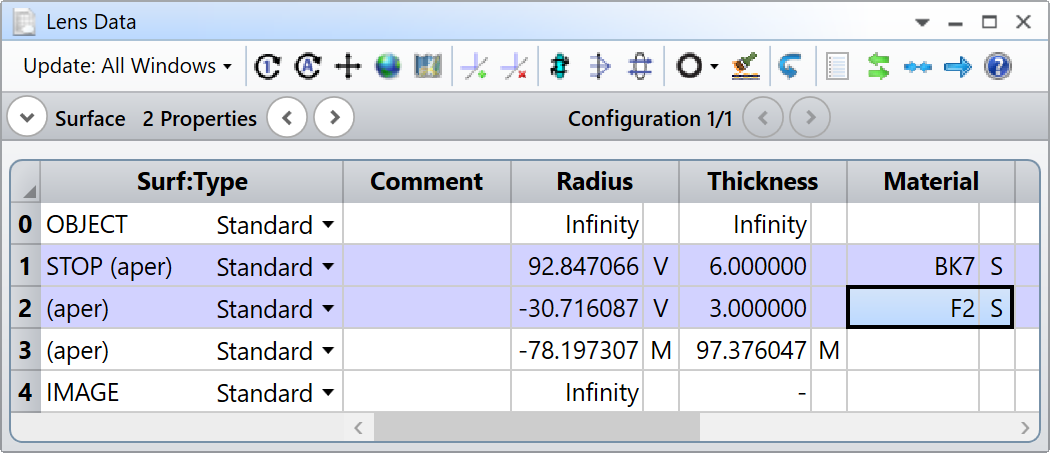
\includegraphics[width=.48\textwidth,height=.24\textheight,keepaspectratio]{Figure/玻璃替换/Picture2zh-cn.png}
                \vspace{4pt}
                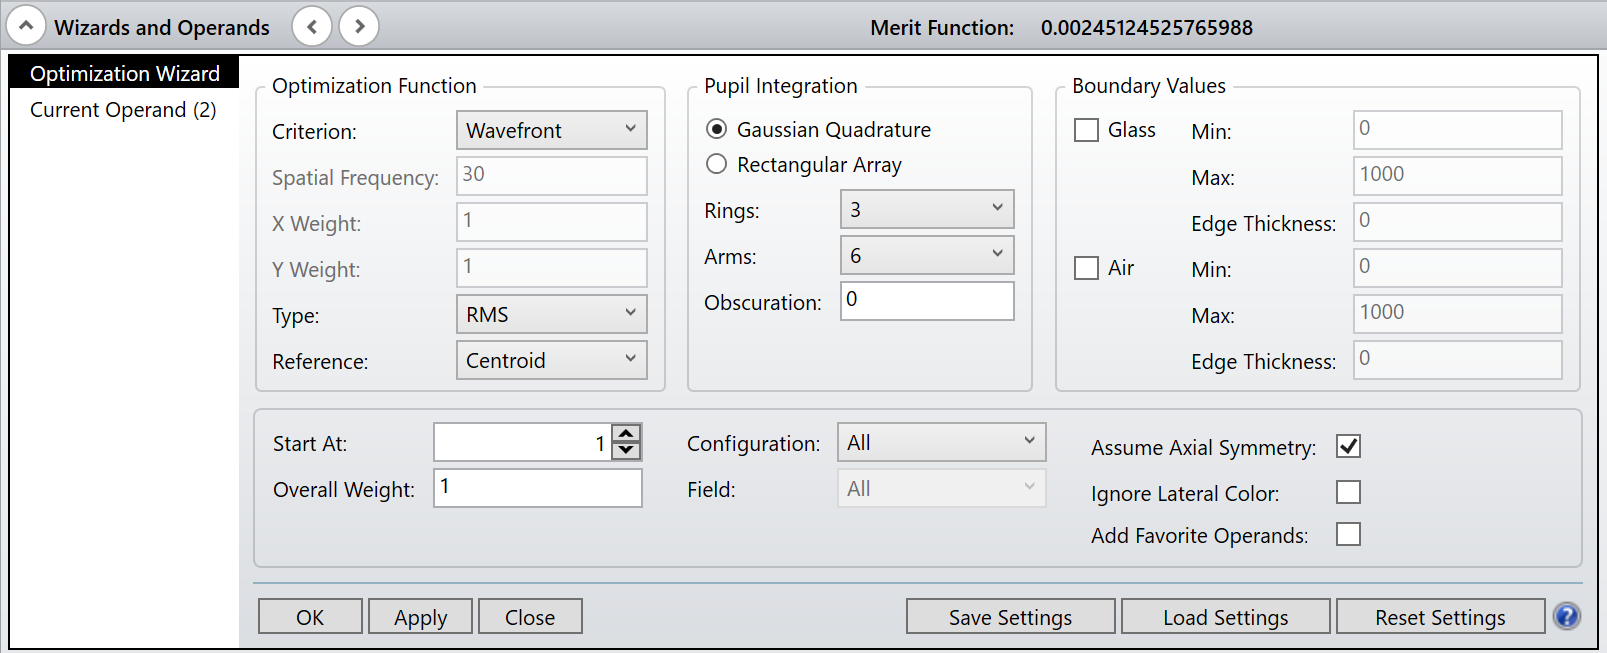
\includegraphics[width=.48\textwidth,height=.24\textheight,keepaspectratio]{Figure/玻璃替换/Picture3zh-cn.png}\hfill
                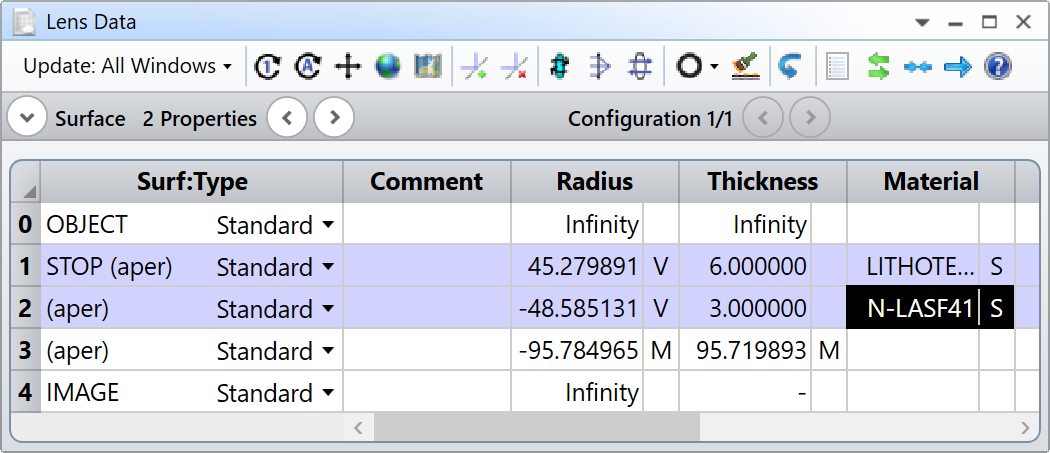
\includegraphics[width=.48\textwidth,height=.24\textheight,keepaspectratio]{Figure/玻璃替换/Picture8zh-cn.png}
                \caption{Substitute solve、评价函数、Hammer 优化与玻璃模板}
                \label{fig:glass_substitution_steps_main}
            \end{figure}
        \end{column}
    \end{columns}
\end{frame}

\subsection{诊断闭环：从图到结论}
\label{sec:1.6}

\englishtitle{Diagnostic Workflow}
\begin{frame}{像差诊断流程：从图到结论}
\label{1.16}
    \begin{columns}[T]
        \begin{column}{.50\textwidth}
            \begin{block}{Ray Fan 先行诊断}
                \begin{enumerate}
                    \item 先看轴上视场：三次曲线为球差，波长斜率差为轴向色差。
                    \item 再看轴外视场：二次曲线为彗差，原点斜率变化为场曲/像散。
                    \item 对比子午和弧矢：斜率分离说明像散。
                    \item 对比不同波长：截距分离说明倍率色差。
                    \item 对比满刻度宽度：光束变窄说明渐晕或光瞳像差。
                \end{enumerate}
            \end{block}
        \end{column}
        \hfill
        \begin{column}{.50\textwidth}
            \begin{block}{再用波前和像质确认}
                \begin{itemize}
                    \item \textbf{Zernike}：分解 OPD，确认主要波前模式。
                    \item \textbf{Spot}：查看几何弥散斑是否落入像元。
                    \item \textbf{PSF}：查看点像能量是否集中。
                    \item \textbf{MTF}：查看目标空间频率的对比度传递。
                    \item \textbf{Encircled Energy}：查看探测器采样能量是否足够。
                \end{itemize}
            \end{block}

            \begin{alertblock}{最重要的工作习惯}
                不要只看一个图下结论；Ray Fan 告诉你“像差形状”，OPD/Zernike 告诉你“波前来源”，MTF/PSF 告诉你“图像后果”。
            \end{alertblock}
        \end{column}
    \end{columns}
\end{frame}
